\documentclass[compress]{beamer}
\usepackage{ifthen,verbatim}

\newcommand{\isnote}{}
\xdefinecolor{lightyellow}{rgb}{1.,1.,0.25}
\xdefinecolor{darkblue}{rgb}{0.1,0.1,0.7}

%% Uncomment this to get annotations
%% \def\notes{\addtocounter{page}{-1}
%%            \renewcommand{\isnote}{*}
%% 	   \beamertemplateshadingbackground{lightyellow}{white}
%%            \begin{frame}
%%            \frametitle{Notes for the previous page (page \insertpagenumber)}
%%            \itemize}
%% \def\endnotes{\enditemize
%% 	      \end{frame}
%%               \beamertemplateshadingbackground{white}{white}
%%               \renewcommand{\isnote}{}}

%% Uncomment this to not get annotations
\def\notes{\comment}
\def\endnotes{\endcomment}

\setbeamertemplate{navigation symbols}{}
\setbeamertemplate{headline}{\mbox{ } \hfill
\begin{minipage}{5.5 cm}
\vspace{-0.75 cm} \small
\end{minipage} \hfill
\begin{minipage}{4.5 cm}
\vspace{-0.75 cm} \small
\begin{flushright}
\ifthenelse{\equal{\insertpagenumber}{1}}{}{Jim Pivarski \hspace{0.2 cm} \insertpagenumber\isnote/\pageref{numpages}}
\end{flushright}
\end{minipage}\mbox{\hspace{0.2 cm}}\includegraphics[height=1 cm]{../cmslogo} \hspace{0.1 cm} \includegraphics[height=1 cm]{../tamulogo} \hspace{0.01 cm} \vspace{-1.05 cm}}

\newcommand{\s}[1]{{\mbox{\scriptsize #1}}}

\begin{document}
\begin{frame}
\vfill
\begin{center}
\textcolor{darkblue}{\Large Muon-Groups Analysis Update}

\vfill
\begin{columns}
\column{0.3\linewidth}
\begin{center}
\large
Jim Pivarski
\end{center}
\end{columns}

\begin{columns}
\column{0.3\linewidth}
\begin{center}
\scriptsize
{\it Texas A\&M University}
\end{center}
\end{columns}

\vfill
16 August, 2010

\end{center}
\end{frame}

%% \begin{notes}
%% \item This is the annotated version of my talk.
%% \item If you want the version that I am presenting, download the one
%% labeled ``slides'' on Indico (or just ignore these yellow pages).
%% \item The annotated version is provided for extra detail and a written
%% record of comments that I intend to make orally.
%% \item Yellow notes refer to the content on the {\it previous} page.
%% \item All other slides are identical for the two versions.
%% \end{notes}

\small

\begin{frame}
\frametitle{Open issues from last time}
\begin{itemize}\setlength{\itemsep}{0.25 cm}
\item We found that the $N_\s{segments} \ge 2$ cut provided
  TrackerMuons with the same background-rejection power as
  GlobalMuons, yet TrackerMuons (even with the cut) have an
  easier-to-understand reconstruction efficiency.
  ``$N_\s{segments}$'' is defined with segment-and-track arbitration.
  \textcolor{darkblue}{Question:} is the two-segment requirement the
  important thing, or is it important that they be arbitrated
  segments? \mbox{\textcolor{darkblue}{(answered in this talk)}}
\item GlobalMuon inefficiency in the endcap is clearly related to
  crossing in the muon system.  GlobalMuon inefficiency in the barrel
  seems to be related to crossing somewhere else.
  \textcolor{darkblue}{Question:} what is barrel GlobalMuon
  inefficiency most strongly correlated with?
  \mbox{\textcolor{darkblue}{(not answered: on the to-do list)}}
\item In the set of quality cuts I used last time, some cuts were
  irrelevant and caused undesirable inefficiencies in displaced
  muon-groups.  \textcolor{darkblue}{Question:} which ones?
  \mbox{\textcolor{darkblue}{(answered in this talk)}}
\end{itemize}
%% \hspace{-0.83 cm} \textcolor{darkblue}{\Large Outline2}
\end{frame}

\begin{frame}
\frametitle{$N_\s{segments}$ and arbitration}

{\scriptsize
\begin{itemize}
\item \textcolor{darkblue}{NoArbitration:} count any segments matched to the track, allowing double-counting of tracks to segments and segments to tracks
\item \textcolor{darkblue}{SegmentArbitration:} count only segment matched as best by $\sqrt{(\Delta x)^2 + (\Delta y)^2}$
\item \textcolor{darkblue}{SegmentAndTrackArbitration:} count only best segment match and best track match: a one-to-one relationship (only option recommended by $\mu$POG)
\end{itemize}}

\only<1>{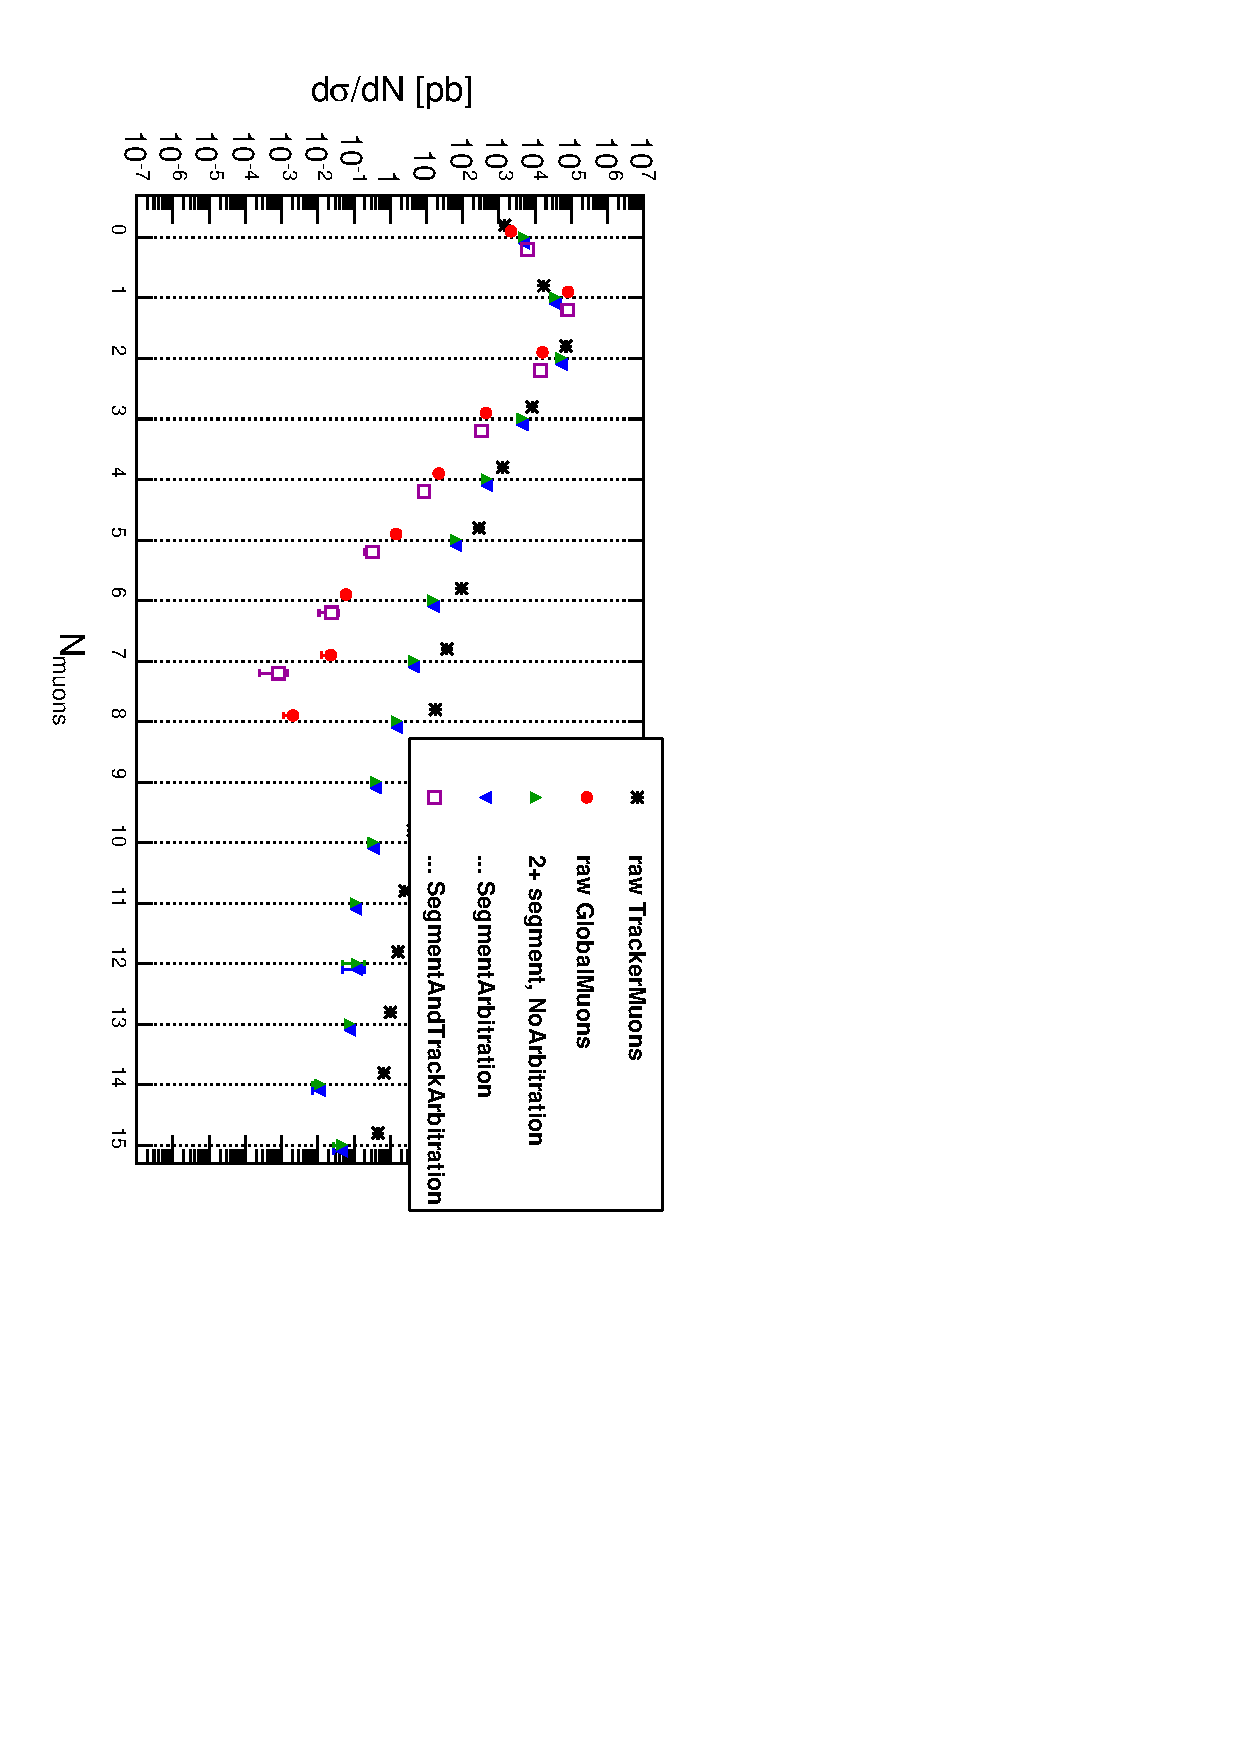
\includegraphics[height=\linewidth, angle=90]{tracks_lastpage_allreal.pdf}}
\only<2>{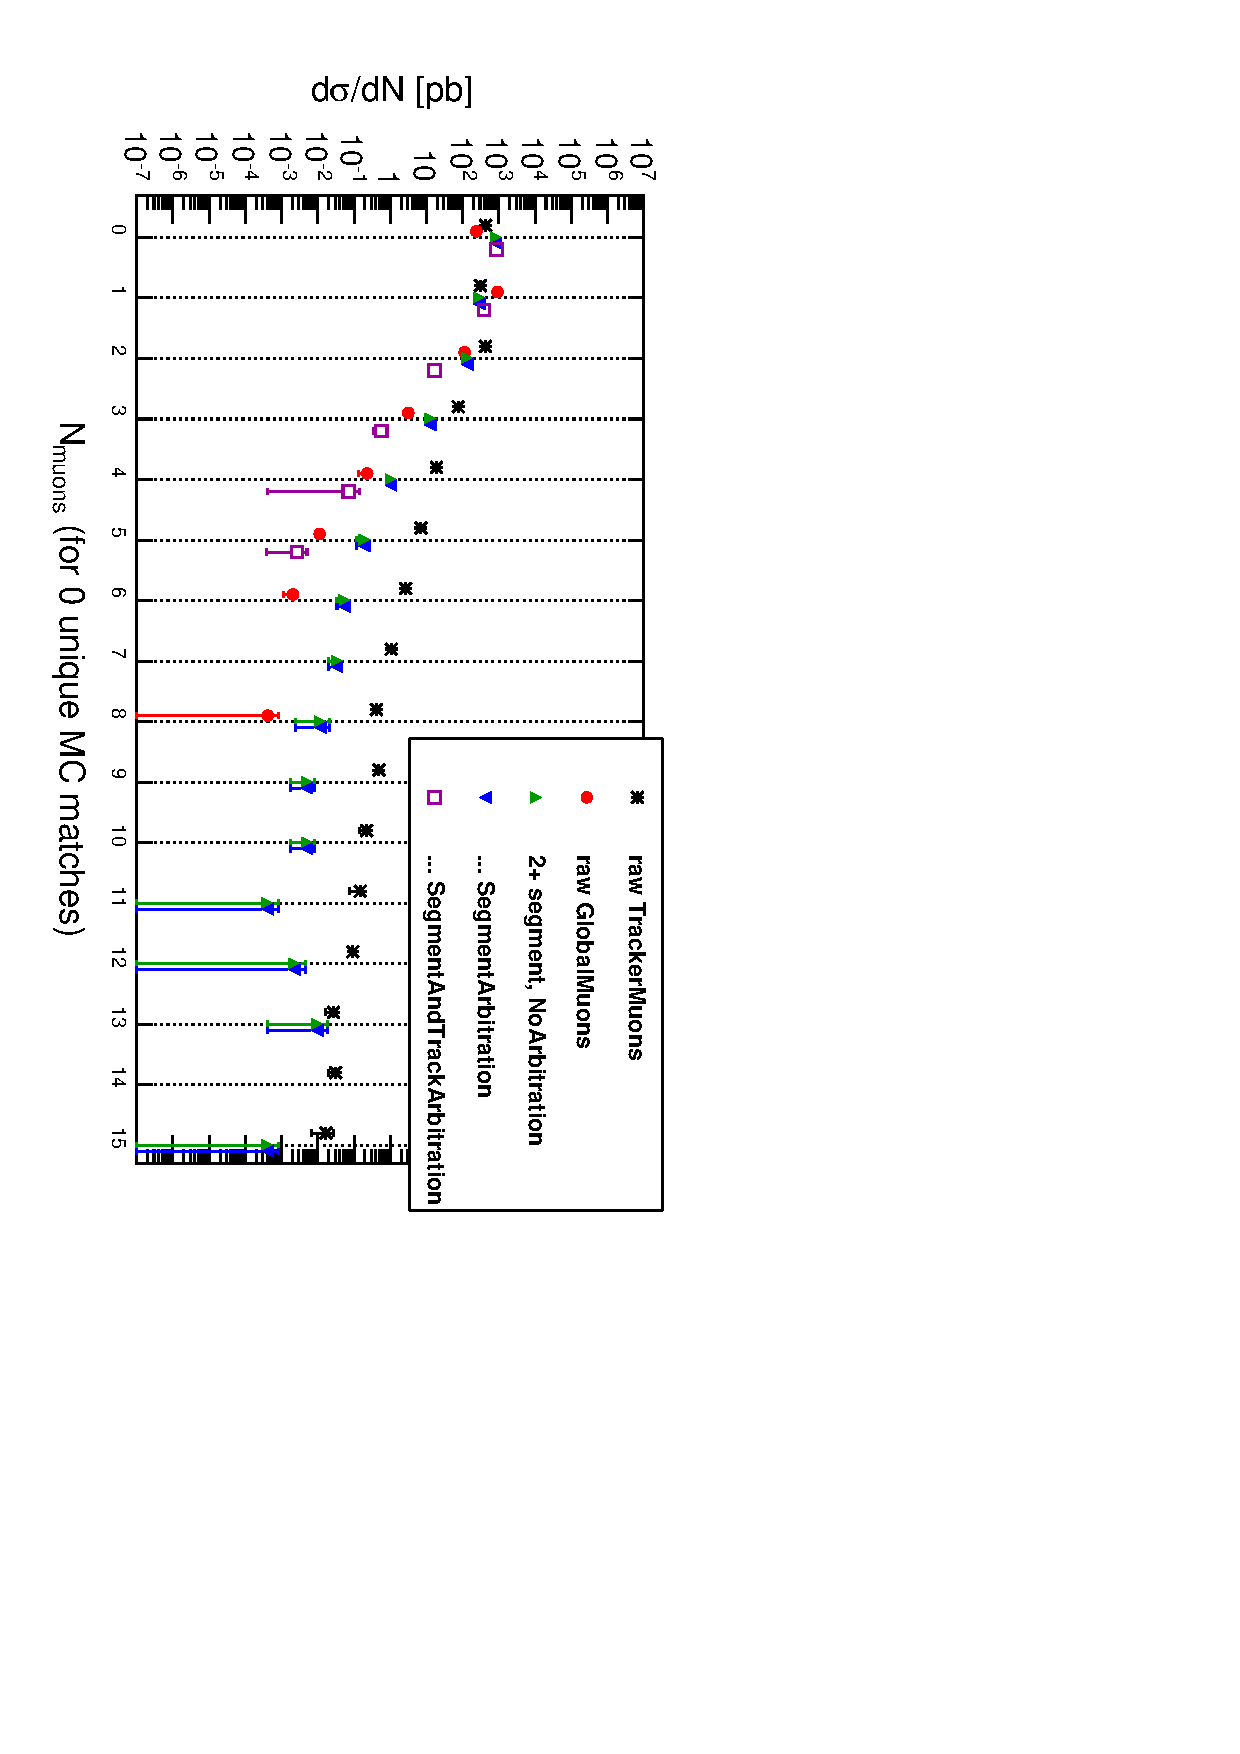
\includegraphics[height=\linewidth, angle=90]{tracks_lastpage_0real.pdf}}
\only<3>{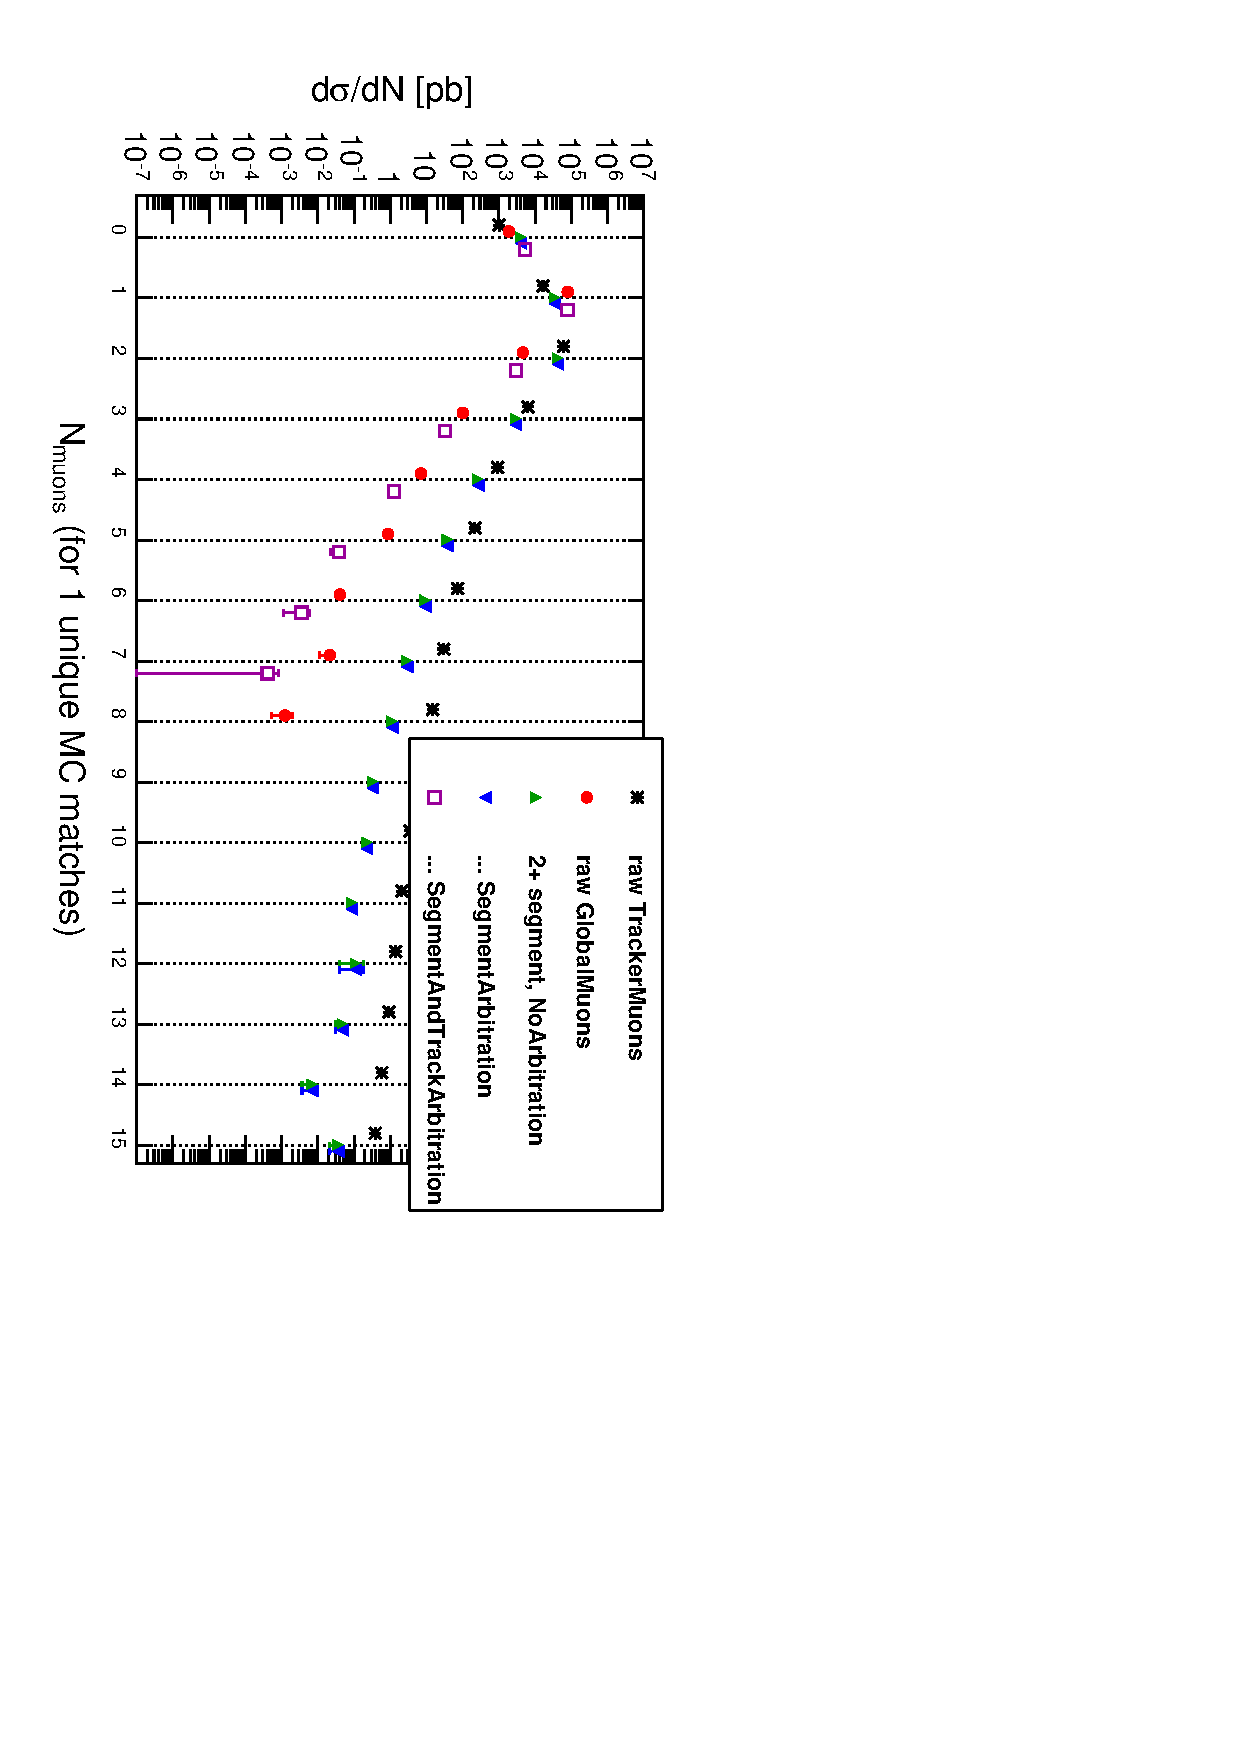
\includegraphics[height=\linewidth, angle=90]{tracks_lastpage_1real.pdf}}
\only<4>{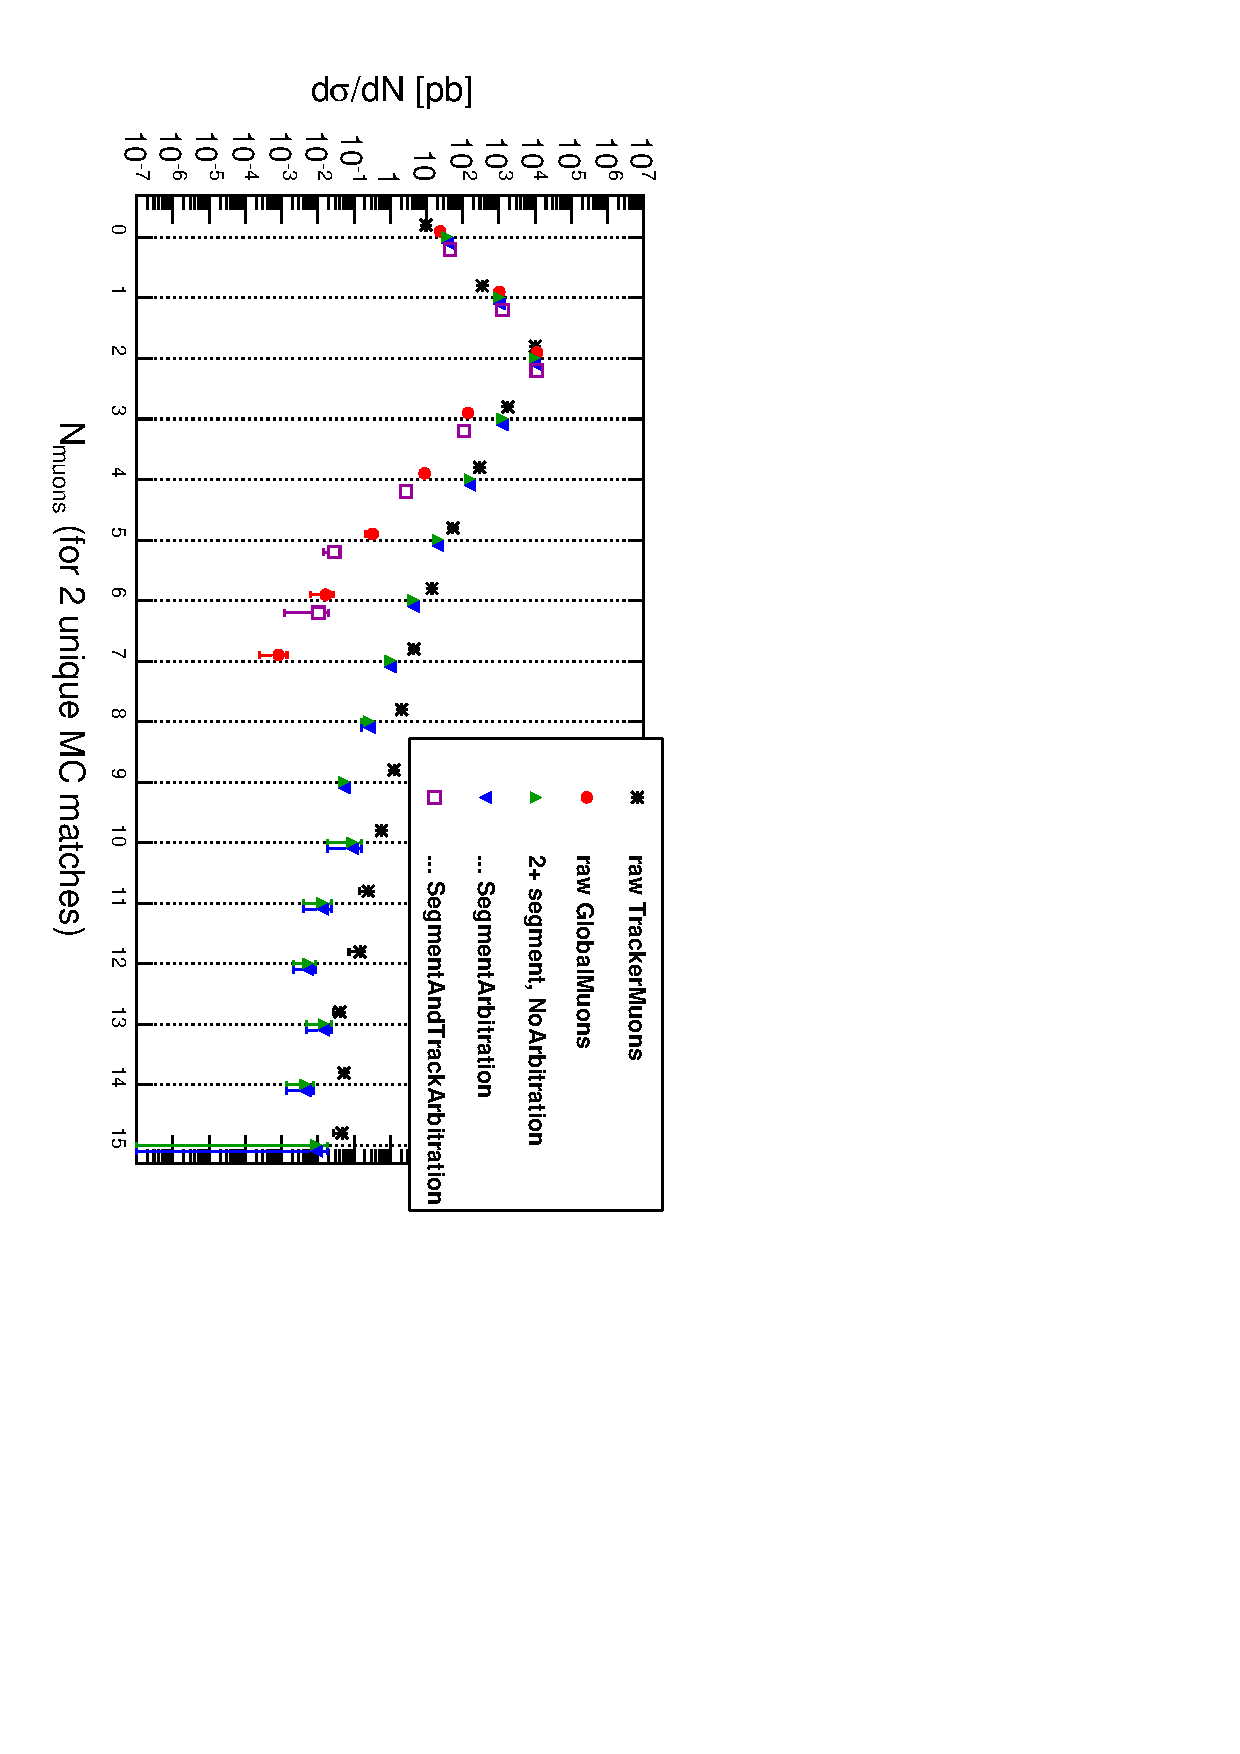
\includegraphics[height=\linewidth, angle=90]{tracks_lastpage_2real.pdf}}
\only<5>{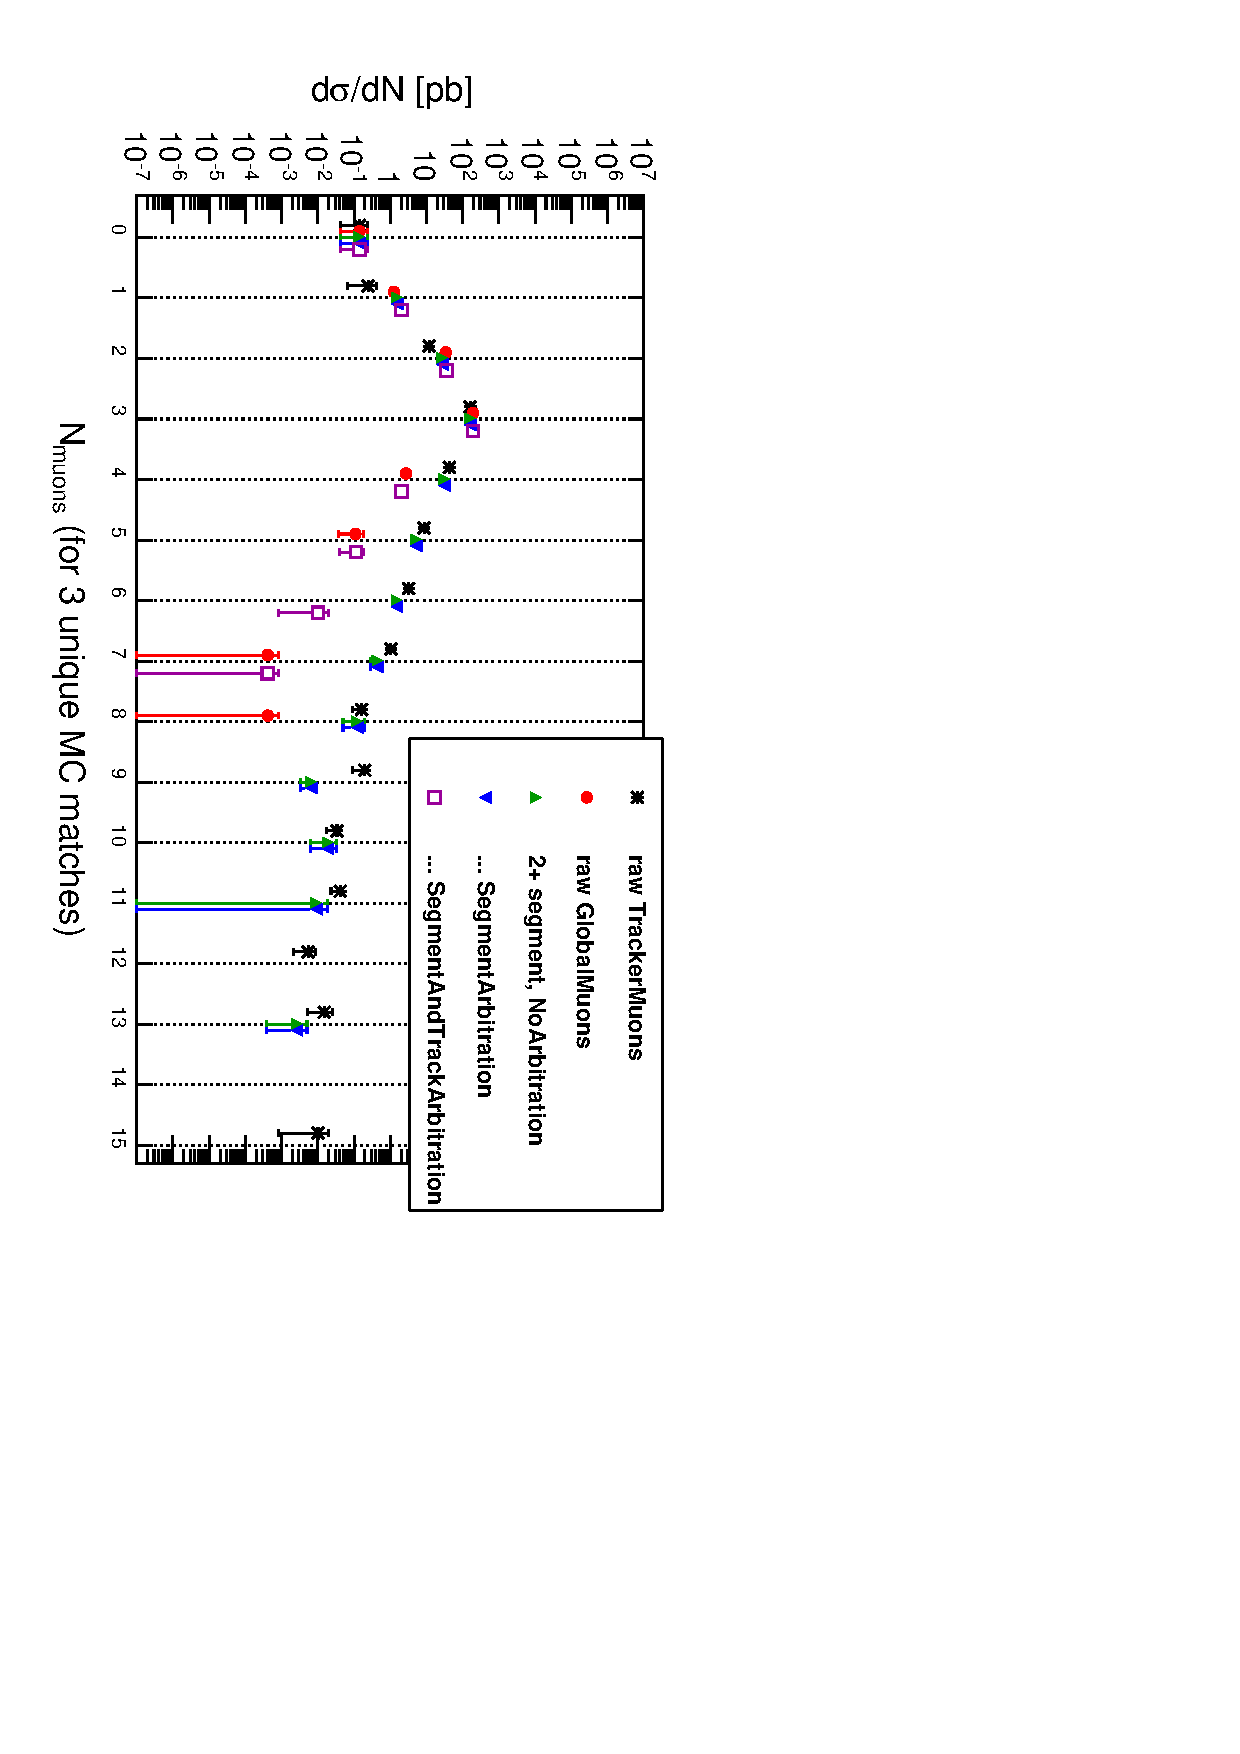
\includegraphics[height=\linewidth, angle=90]{tracks_lastpage_3real.pdf}}
\only<6>{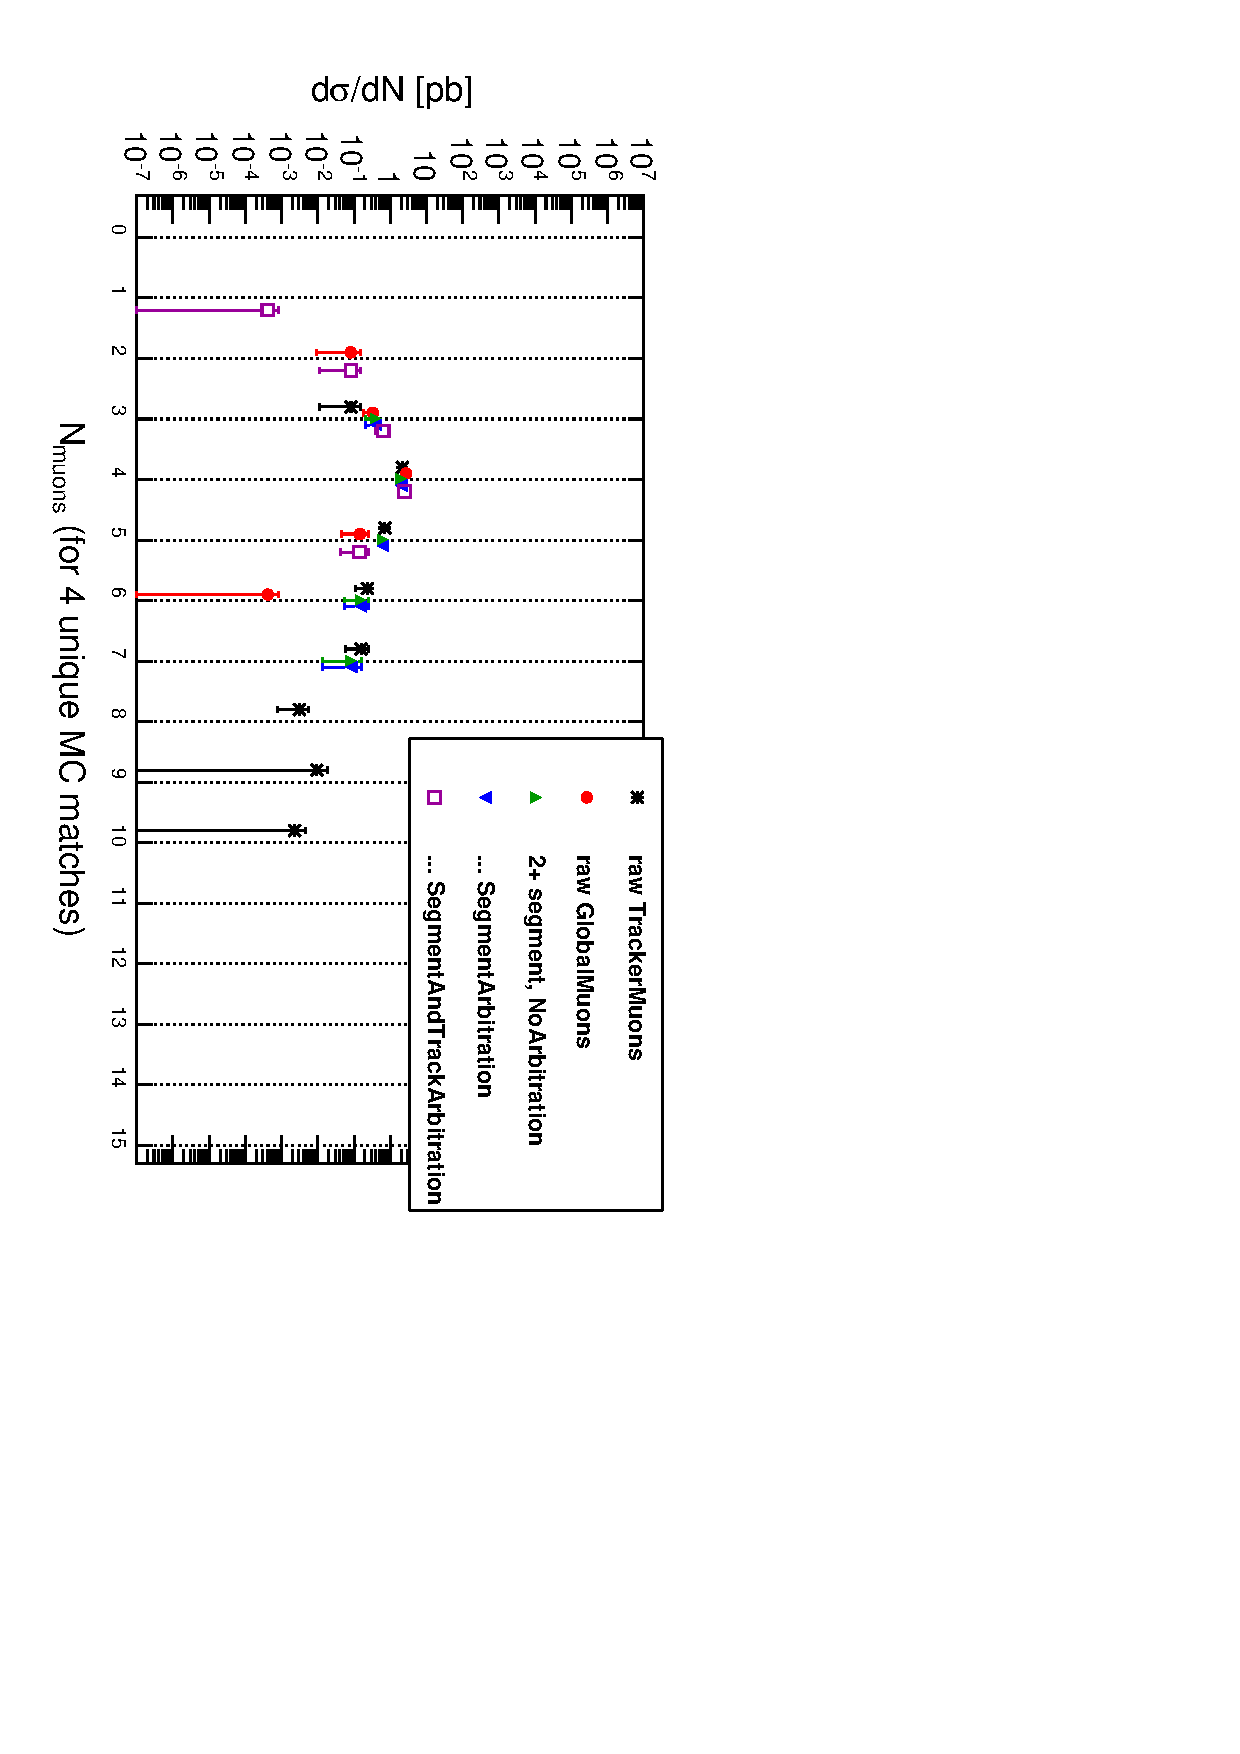
\includegraphics[height=\linewidth, angle=90]{tracks_lastpage_4real.pdf}}
\only<7>{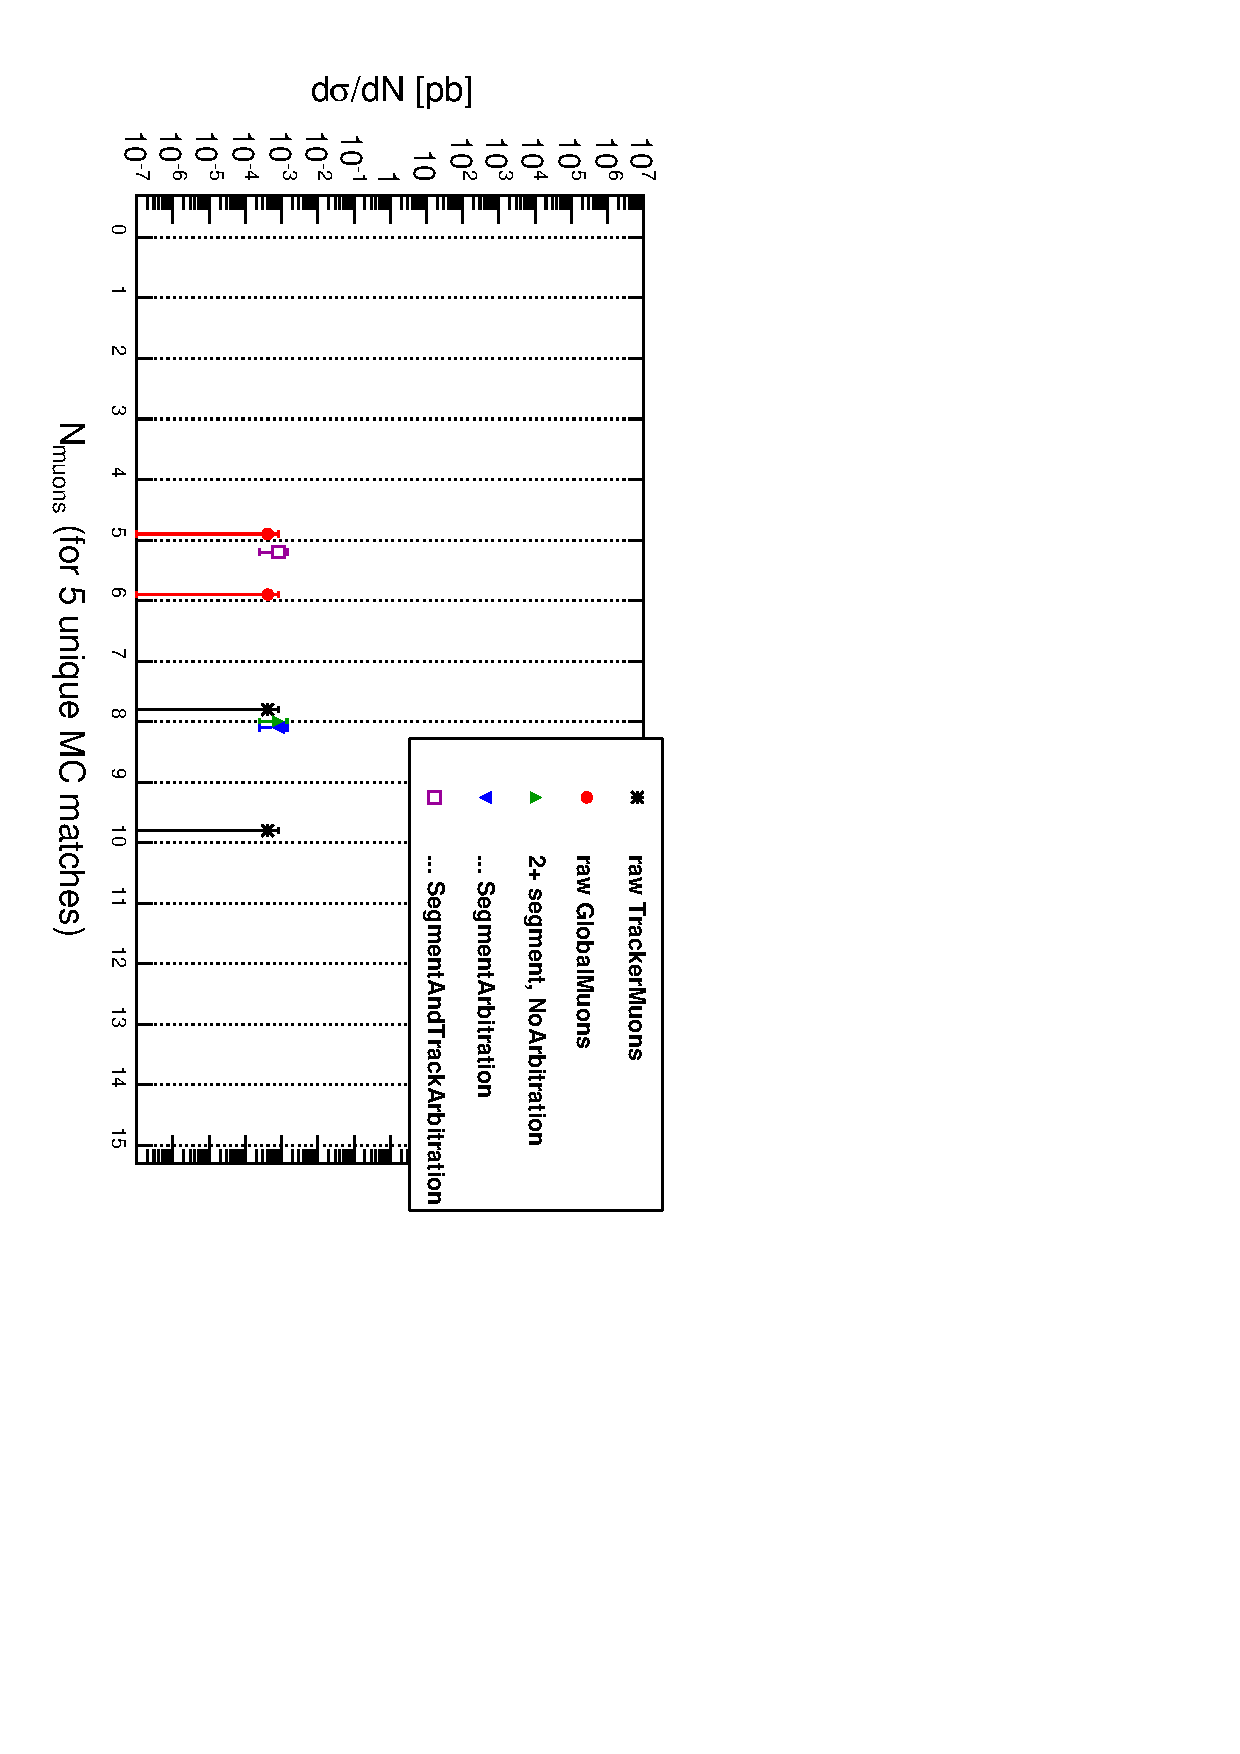
\includegraphics[height=\linewidth, angle=90]{tracks_lastpage_5real.pdf}}
\end{frame}

\begin{frame}
\frametitle{How is MC-matching done?}
\framesubtitle{(also an open question; I've since looked it up)}
\begin{itemize}
\item Standard PAT-muon MC-matching uses the following algorithm:
\begin{enumerate}
\item compare list of reconstructed muons with list of (stable) generator-level muons
\item exclude any potential matches with $\Delta R > 0.5$, $\Delta p_T/p_T > 0.5$, or the wrong charge
\item resolve all ambiguities by $\Delta R$ (no more than one
  reco-muon may match to a gen-muon, no more than one gen-muon may
  match to a reco-muon)
\end{enumerate}

\item Ambiguity resolution is done in the order that muons appear in
  the event (i.e.\ random or with an unknown correlation to some
  parameters): could be better to turn on {\tt resolveByMatchQuality}
  which would resolve in the order of increasing $\Delta R$
\begin{itemize}
\item I'd need to re-run over all samples to turn this option on (I'll
  do it on the next major re-run; e.g. when updating to a newer CMSSW
  version)
\end{itemize}
\end{itemize}
\end{frame}

\begin{frame}
\frametitle{Settling on a standard set of cuts}

\begin{itemize}
\item Event:
\begin{itemize}
\item HLT\_Mu9 (lowest threshold that is not currently prescaled)
\item one muon with $p_T > 11$~GeV/$c$
\item minimum number of muons for desired number of muon-groups
  (e.g.\ at least 4 muons for 2 muon-groups)
\end{itemize}

\item Muon (applied {\it before} our analysis):
\begin{itemize}
\item $|\vec{p}| > 2.5$~GeV/$c$ (TrackerMuon identification)
\item $\ge 8$ tracker hits (not strictly; applied by whom? track-finding?)
\end{itemize}

\item Muon (applied {\it by} our analysis):
\begin{itemize}
\item $p_T > 5$~GeV/$c$, $|\eta| < 2.4$ (tighter than defaults)
\item $N_\s{segments} \ge 2$ with track-and-segment arbitration, $|\Delta x| < 3$~cm, $|\Delta x| < 4 \sigma_{\Delta x}$, $|\Delta y| < 5$~cm, $|\Delta y| < 5 \sigma_{\Delta y}$
\end{itemize}

\item Muon cuts considered, but they don't improve MC performance:
\begin{itemize}
\item tracker $\chi^2/N_\s{dof} < 5$
\item $\sigma_\phi < 0.03$, $\sigma_\eta < 0.01$, $\sigma_{dxy} < 0.05$~cm, $\sigma_{dz} < 0.1$~cm
\item for GlobalMuons: tracker-standAlone matching $\chi^2/N_\s{dof} < 5$
\end{itemize}
\end{itemize}
\end{frame}

\begin{frame}
\frametitle{Checking cut performance}

\begin{itemize}
\item Already verified that $N_\s{segments} \ge 2$ (arbitrated) is the
  only cut that visibly improves TrackerMuon background rejection for
  \mbox{{\it prompt} muons\hspace{-1 cm}}

\item Last time, a cut-off in efficiency for highly displaced vertices
  was observed when requiring all considered cuts: which one?
\end{itemize}

\only<1>{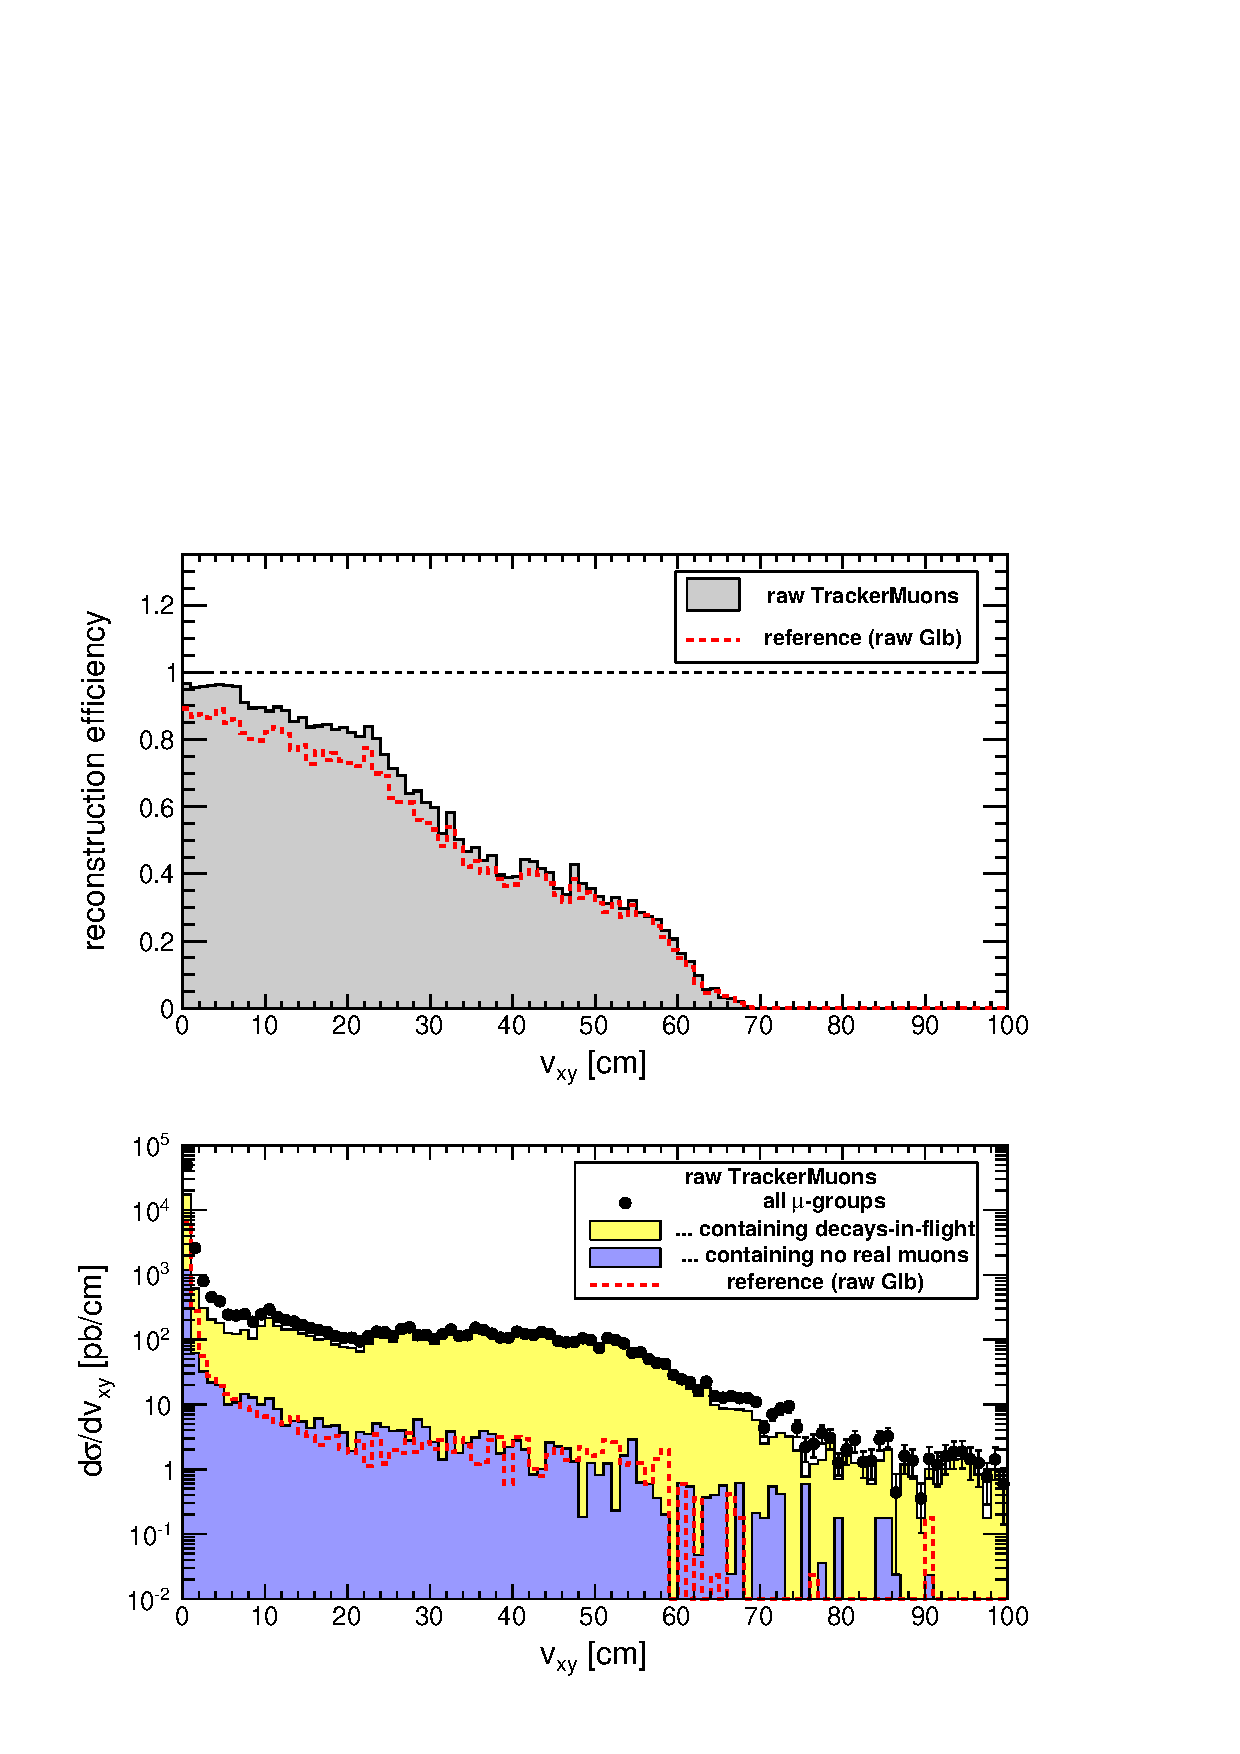
\includegraphics[width=0.49\linewidth]{dispvert_Tracker.pdf}
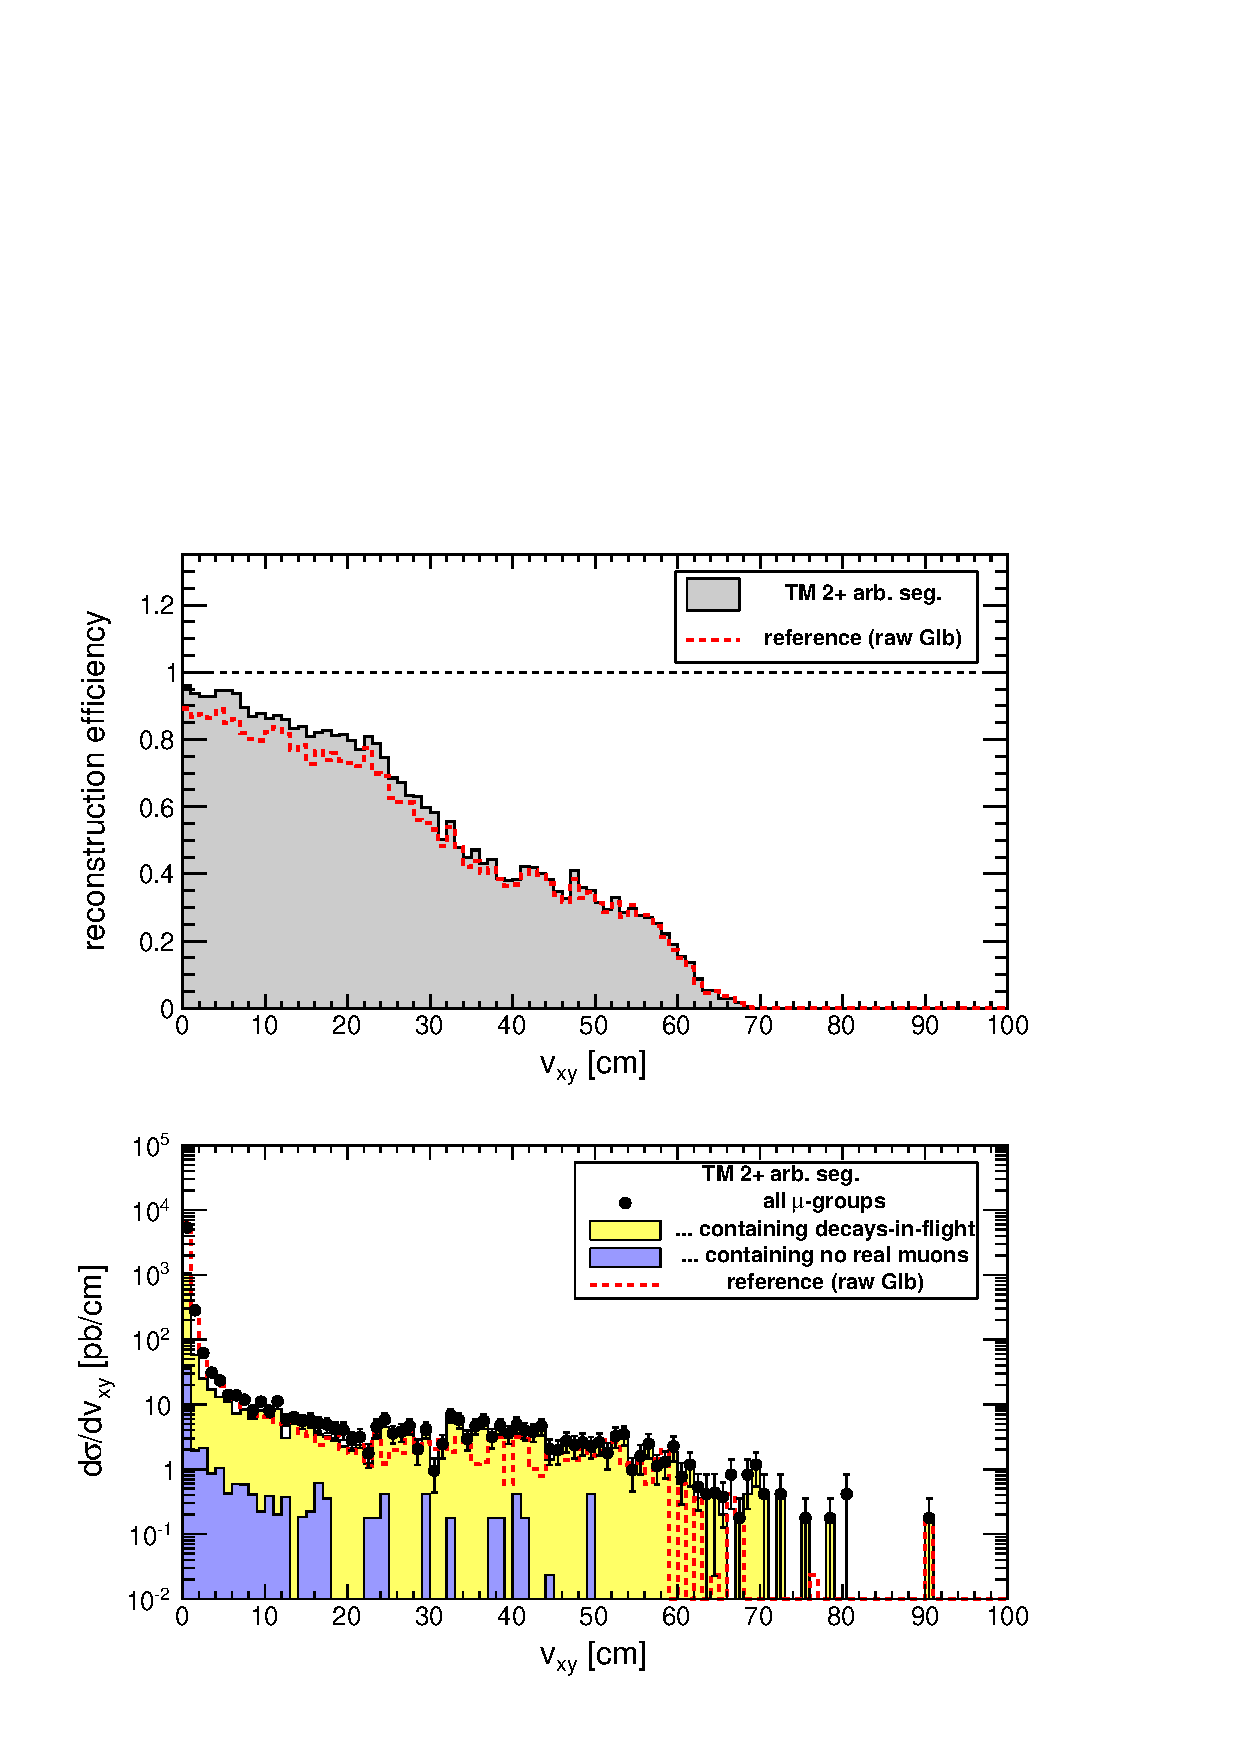
\includegraphics[width=0.49\linewidth]{dispvert_TrackerSegMatch2.pdf}}
\only<2>{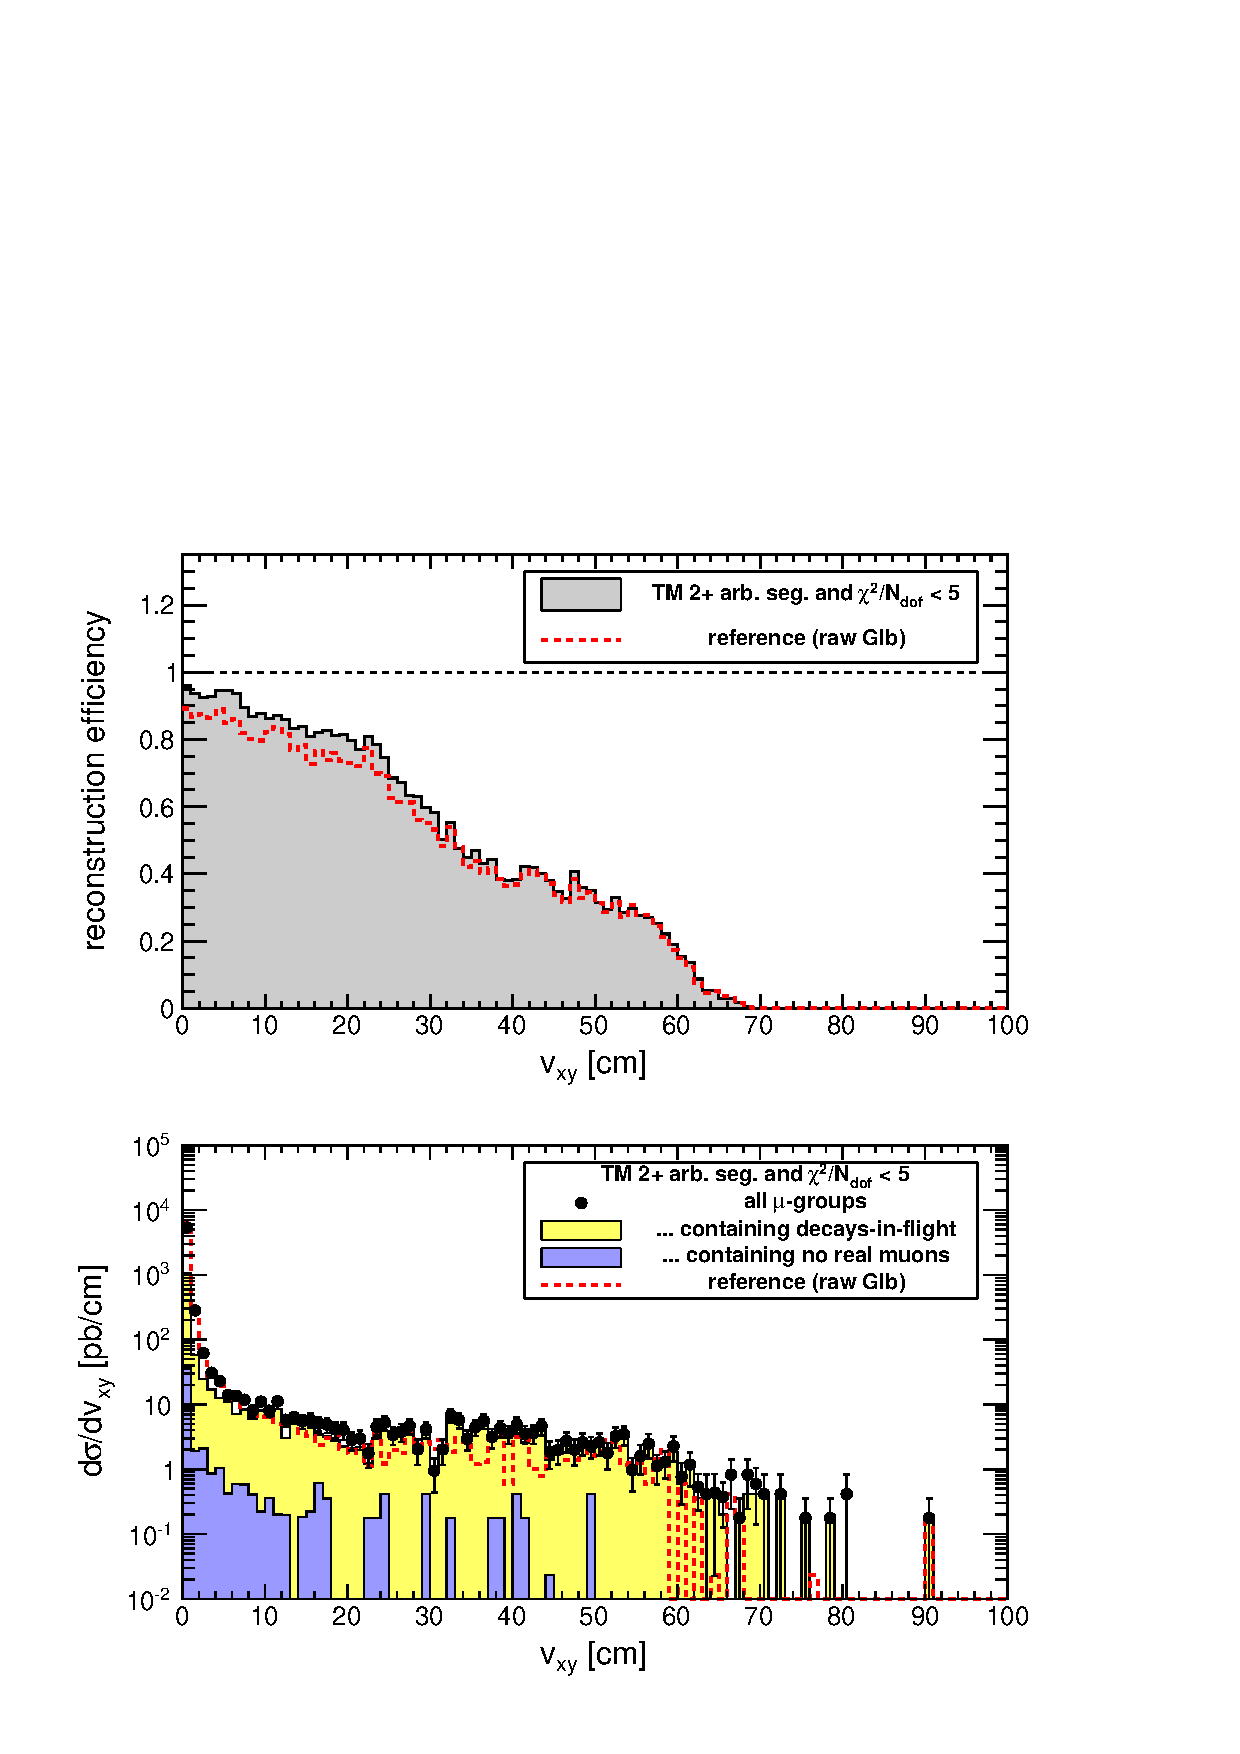
\includegraphics[width=0.49\linewidth]{dispvert_TrackerSegMatch2NormChi2.pdf}
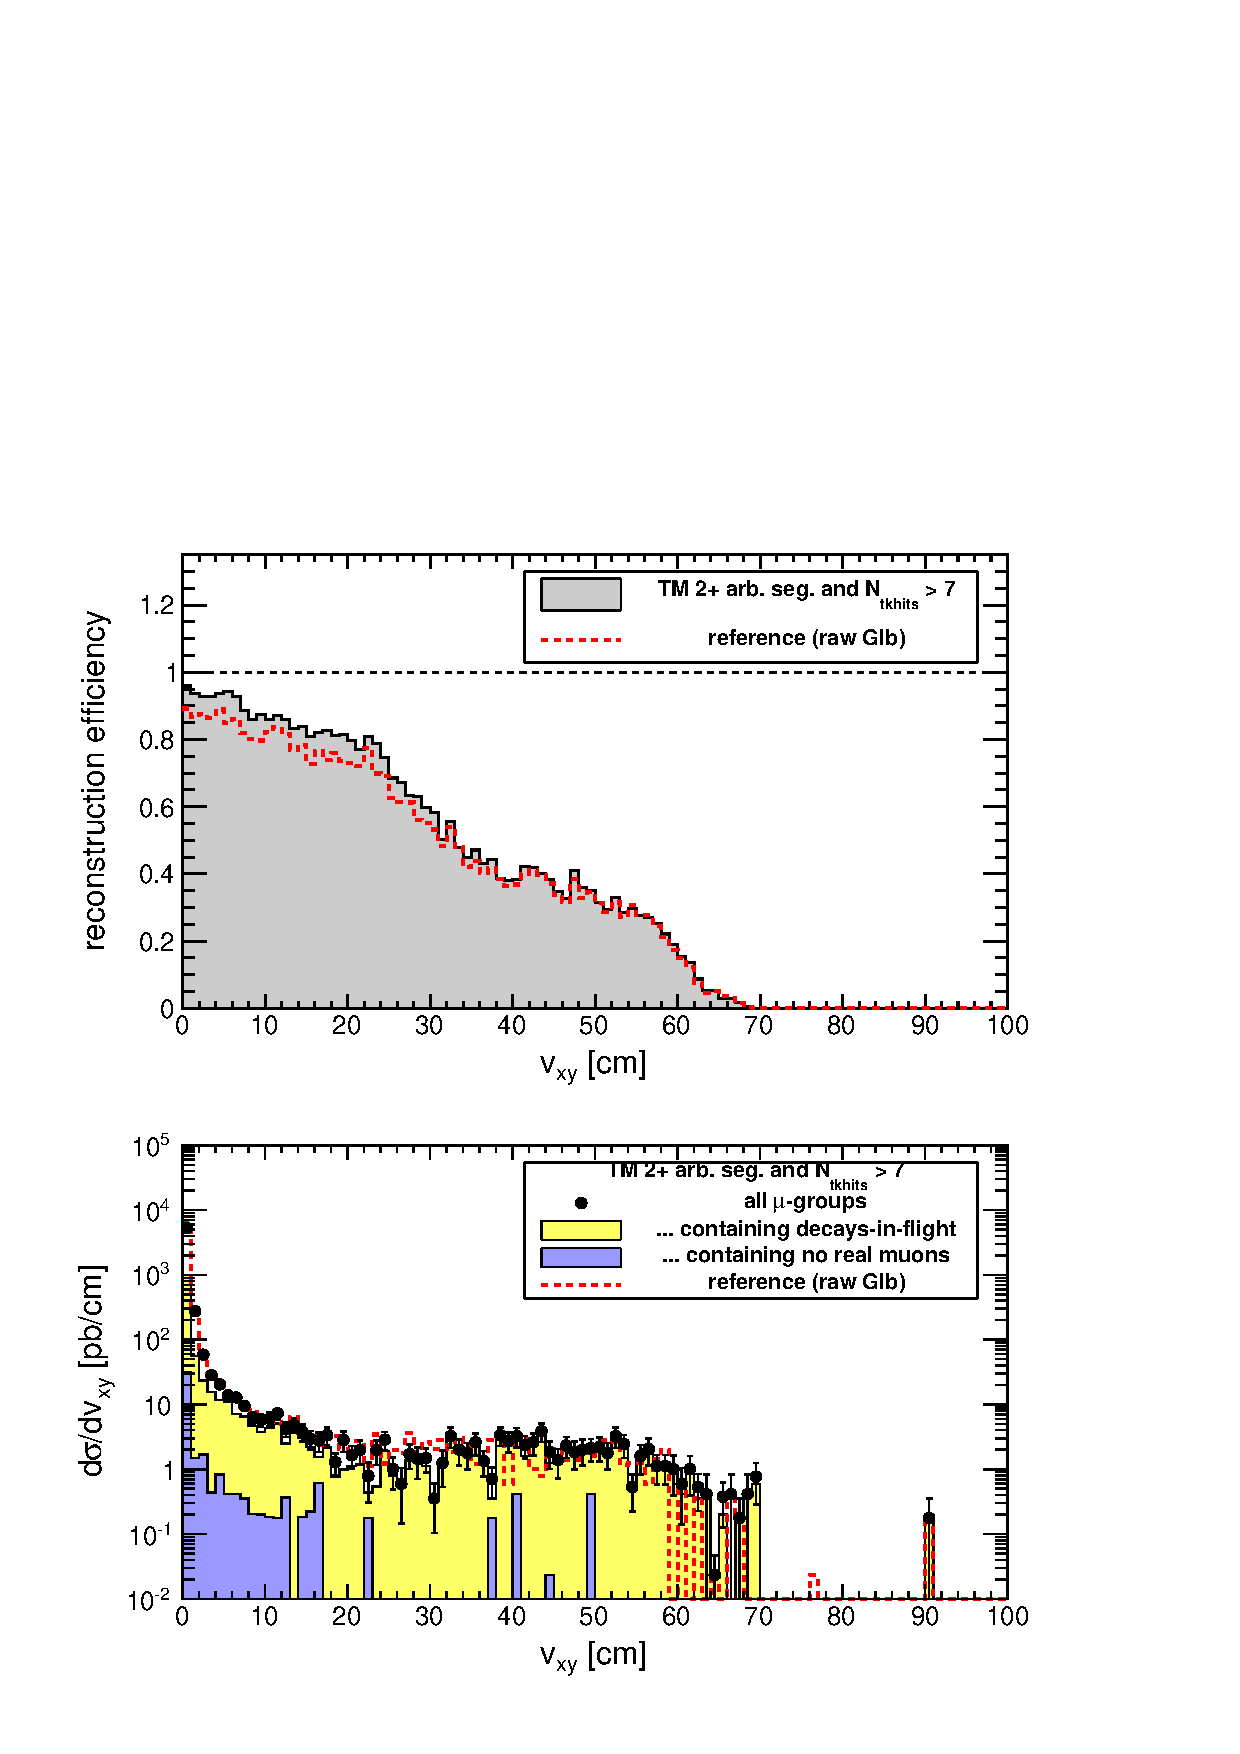
\includegraphics[width=0.49\linewidth]{dispvert_TrackerSegMatch2MinHits.pdf}}
\only<3>{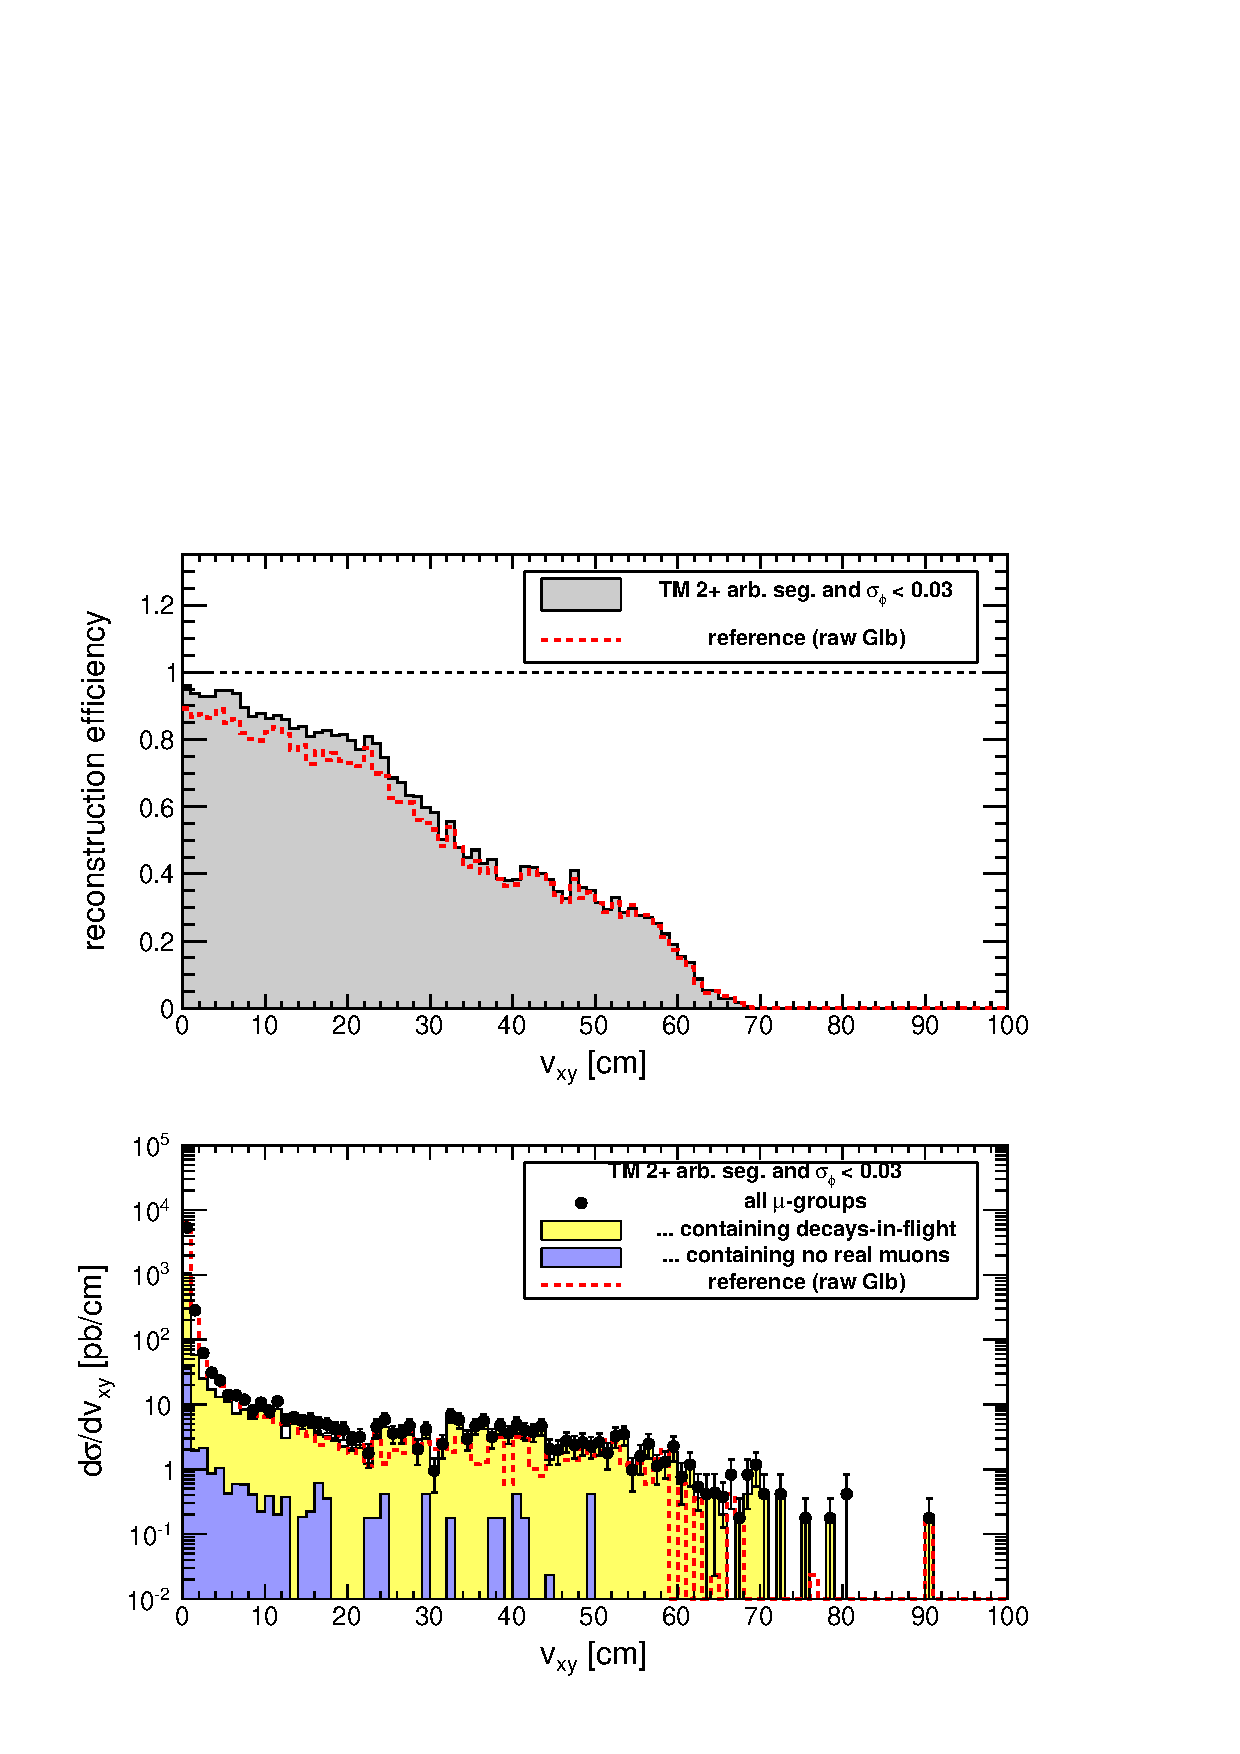
\includegraphics[width=0.49\linewidth]{dispvert_TrackerSegMatch2PhiErr.pdf}
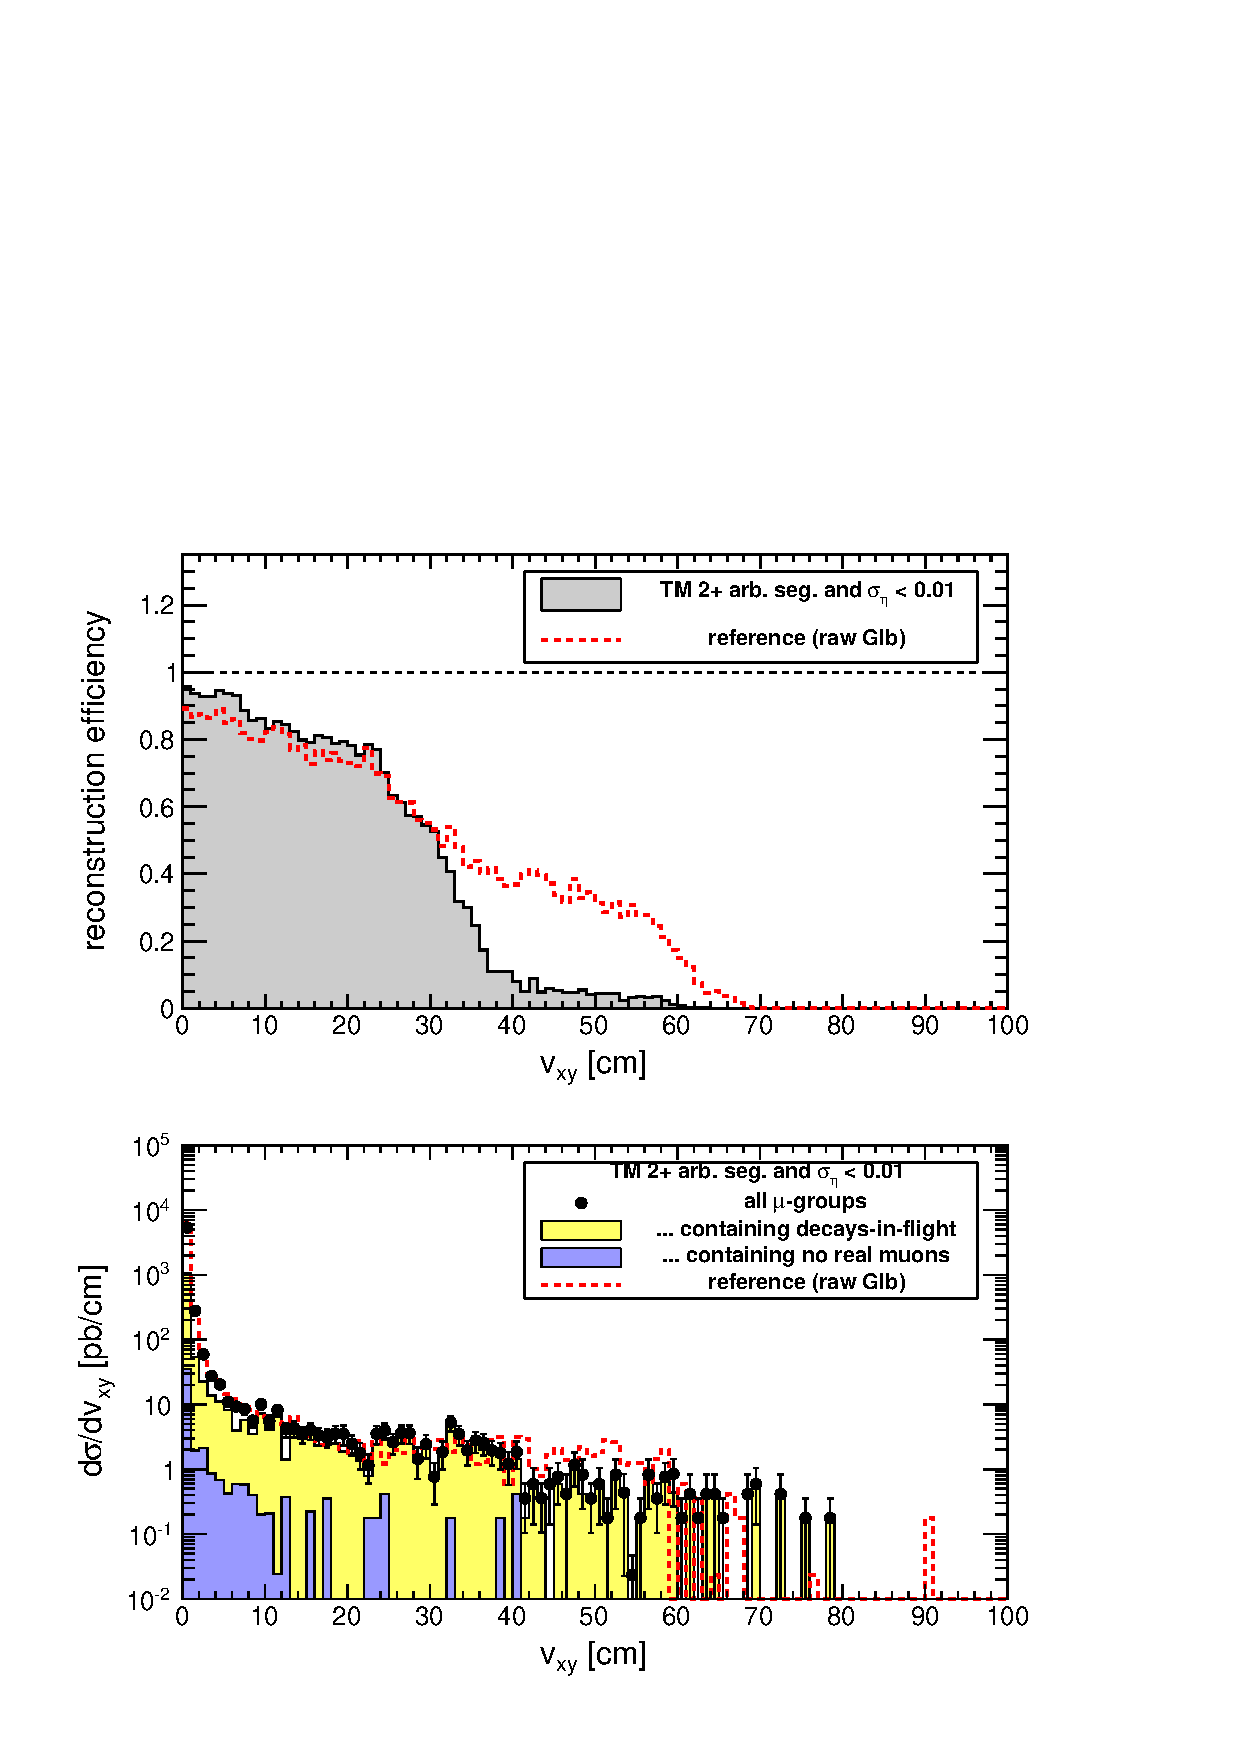
\includegraphics[width=0.49\linewidth]{dispvert_TrackerSegMatch2EtaErr.pdf}}
\only<4>{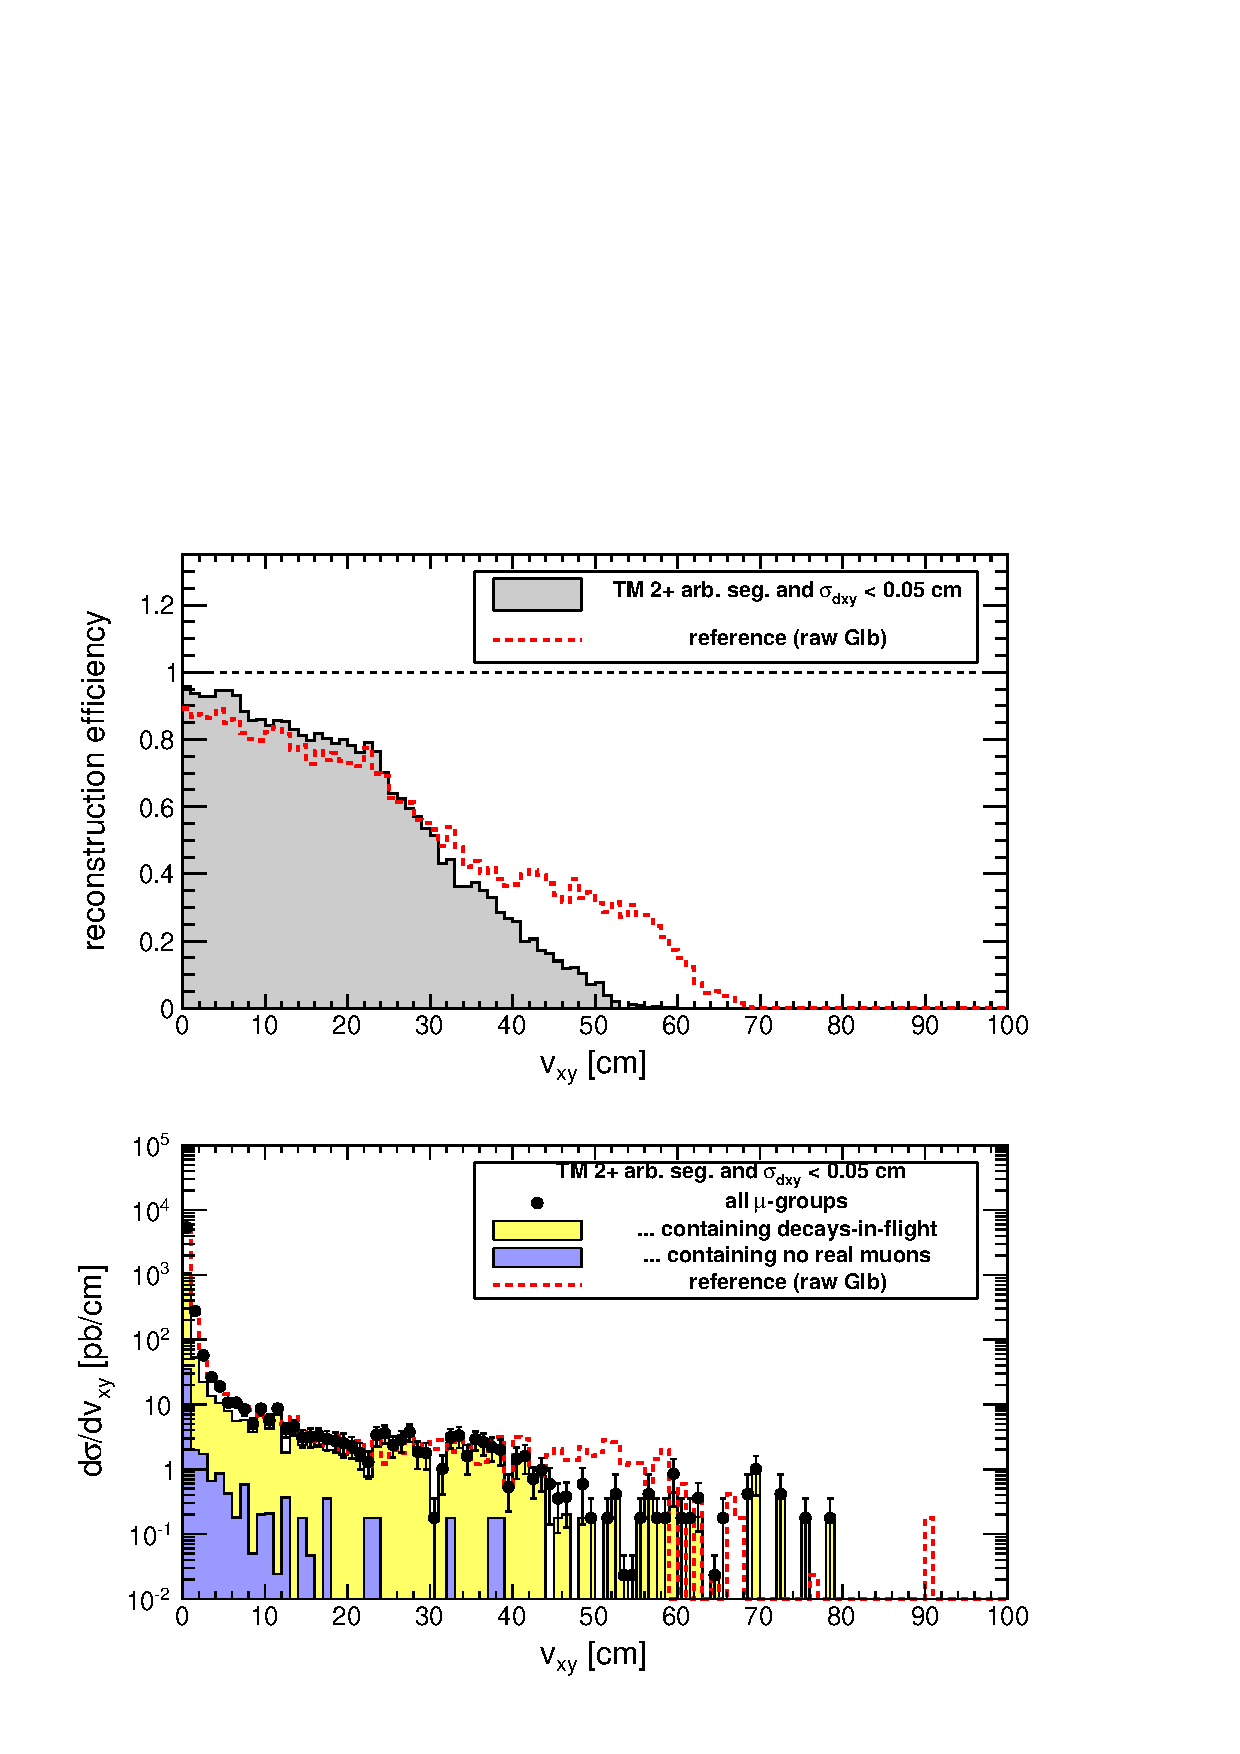
\includegraphics[width=0.49\linewidth]{dispvert_TrackerSegMatch2DxyErr.pdf}
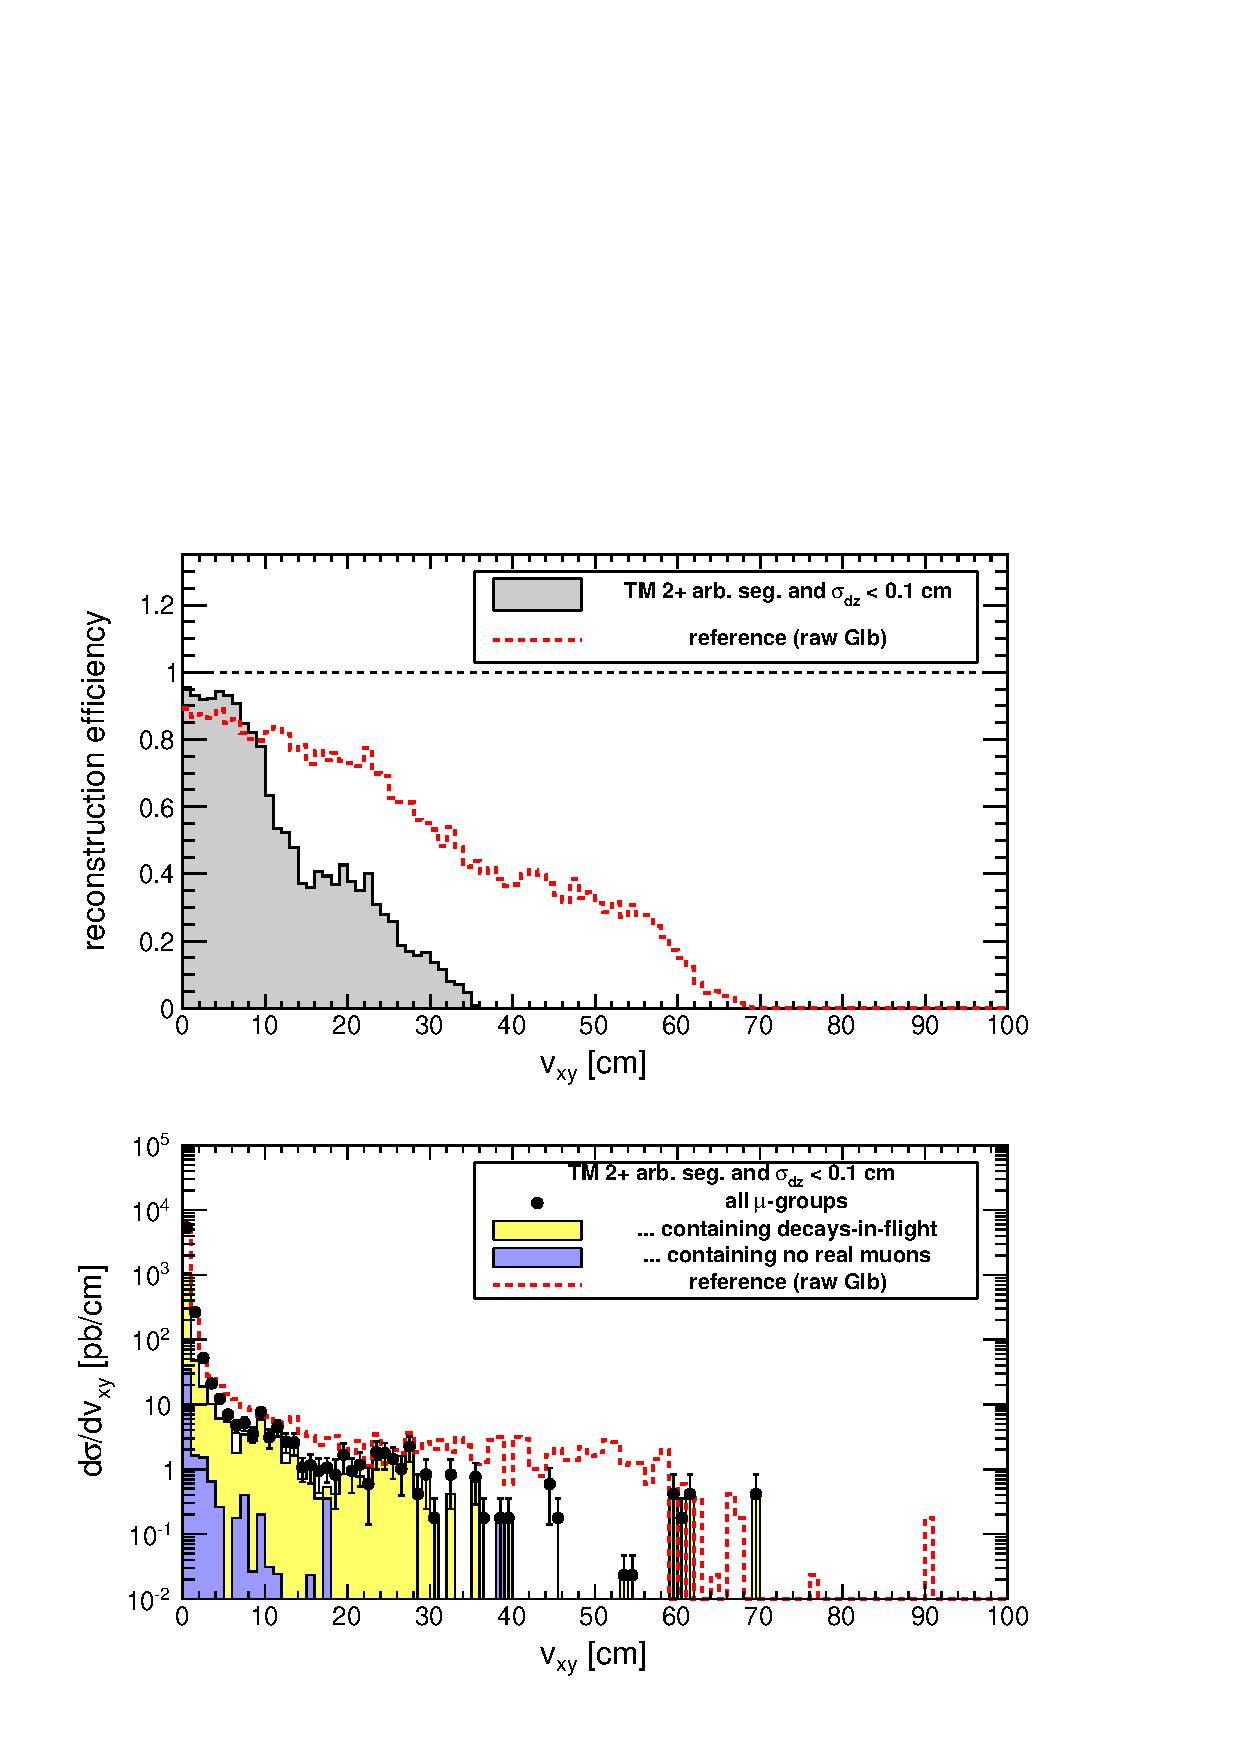
\includegraphics[width=0.49\linewidth]{dispvert_TrackerSegMatch2DzErr.pdf}}
\only<5>{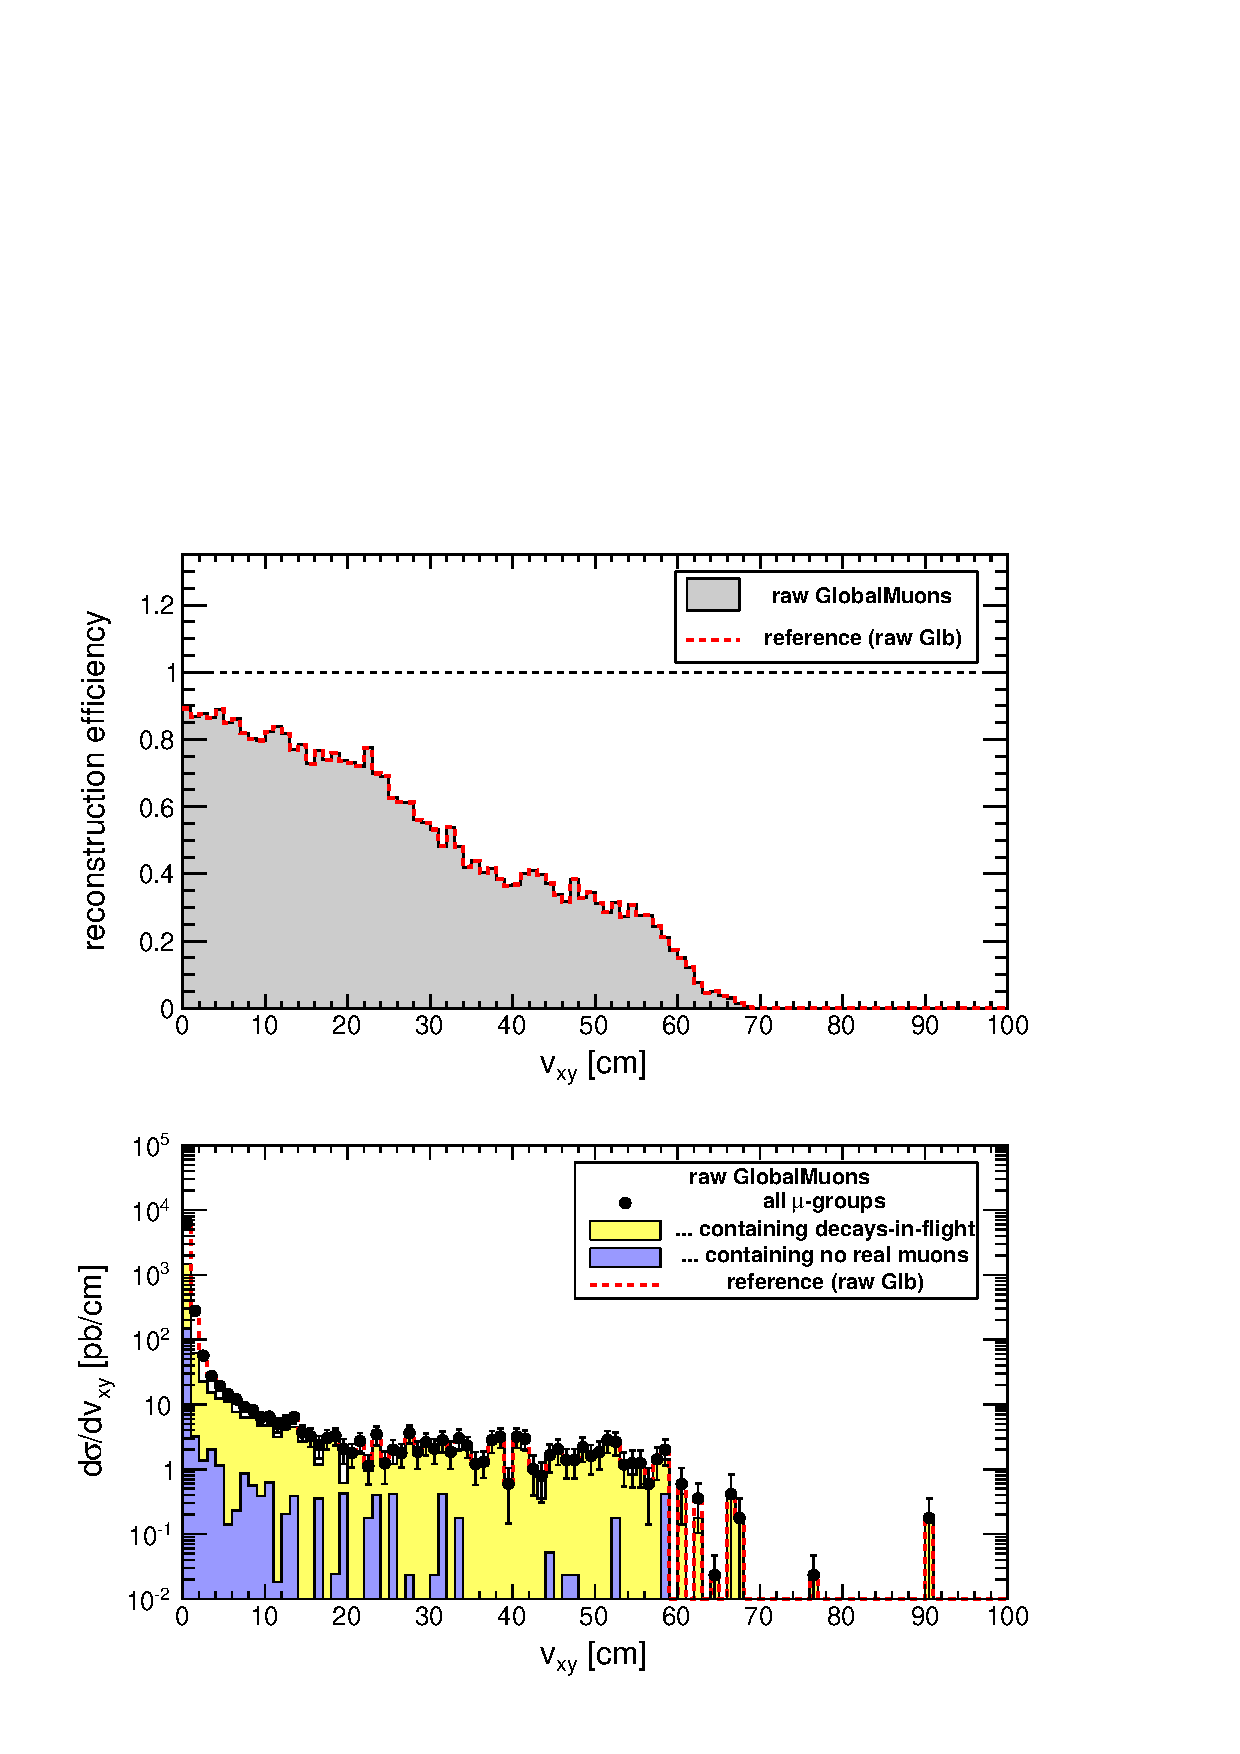
\includegraphics[width=0.49\linewidth]{dispvert_Global.pdf}
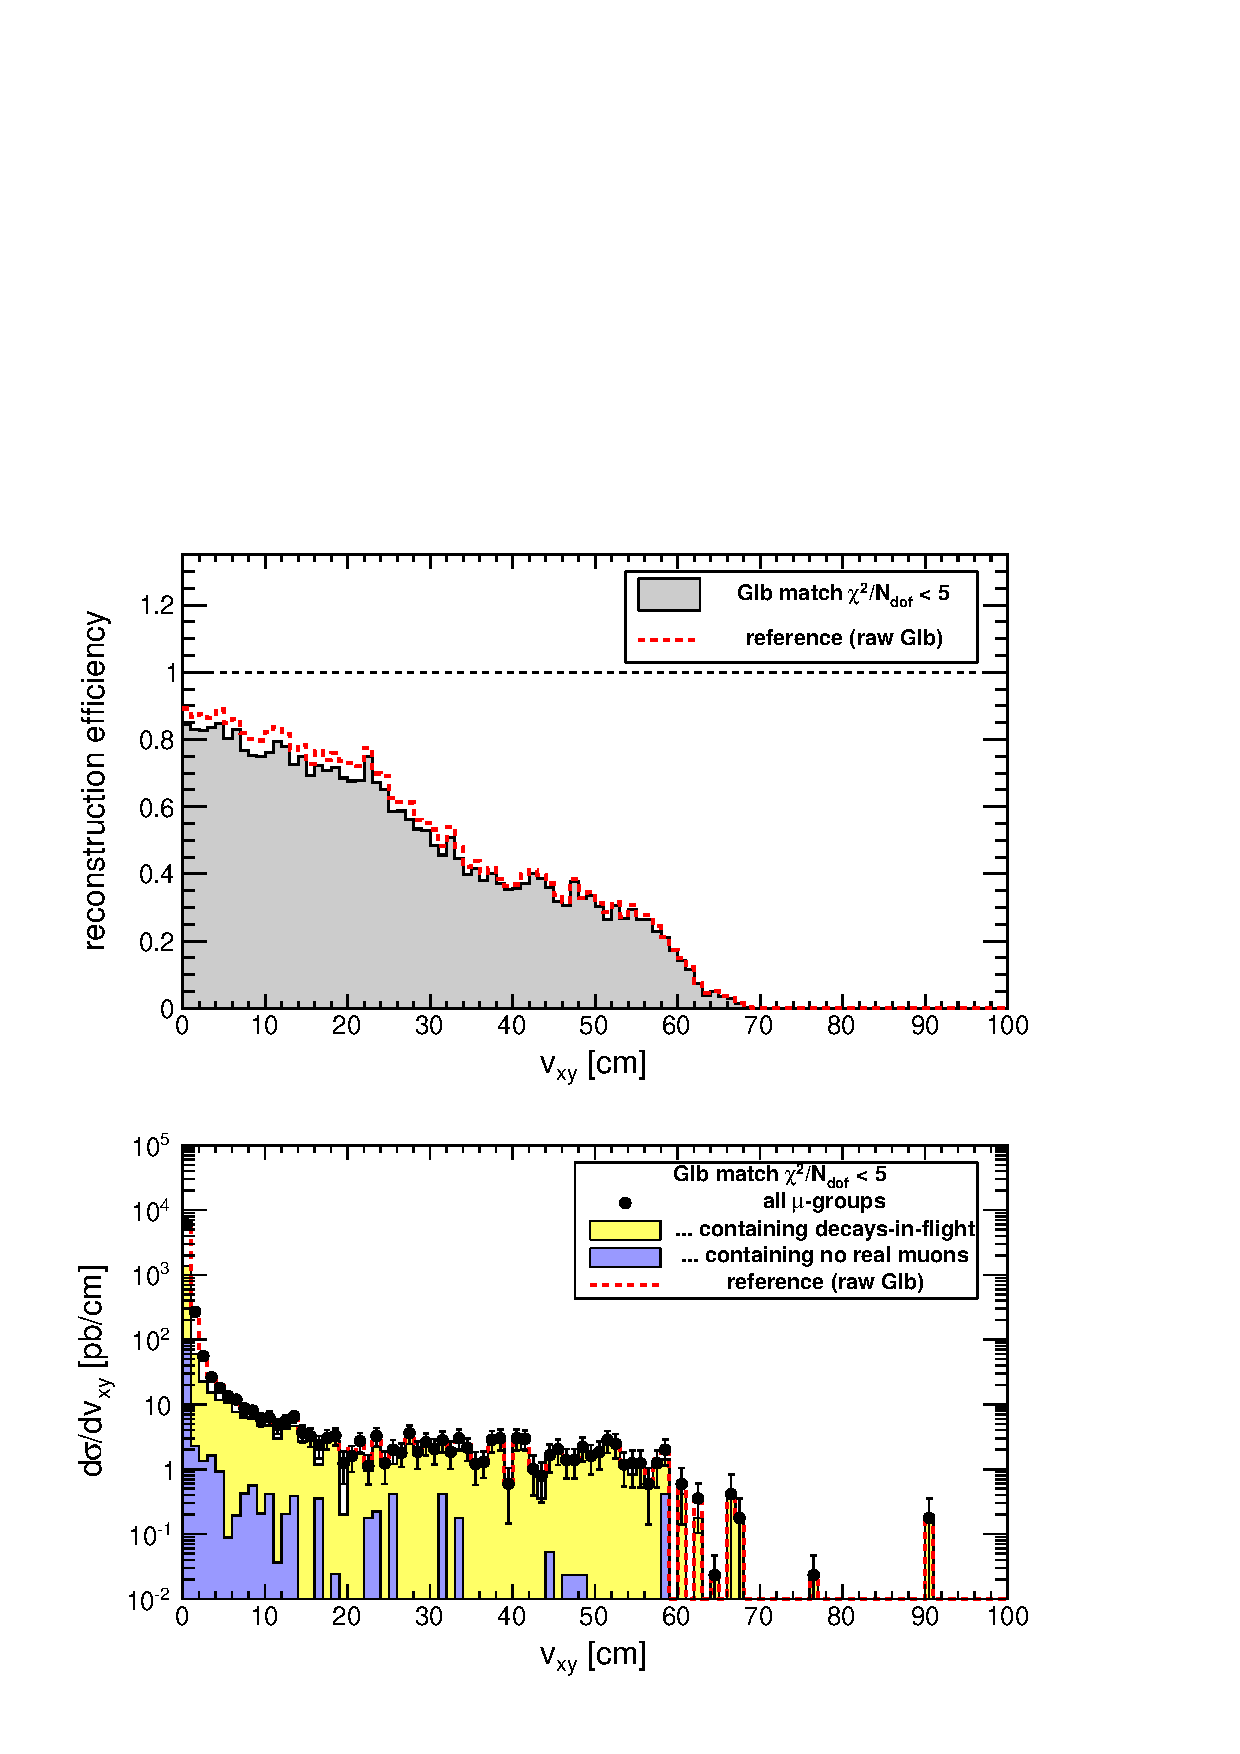
\includegraphics[width=0.49\linewidth]{dispvert_GlobalStaRelChi2.pdf}}
\end{frame}

\begin{frame}
\frametitle{Distributions of cut variables}

\begin{itemize}
\item Linear scale on left; log scale on right
\item Showing both a purely prompt sample (filled) and samples with displaced vertices (the distribution for each $v_{xy}$ range is normalized to the prompt sample)
\item All samples are uniform in pair mass 0--5~GeV/$c^2$, pair $p_T$ 0--100~GeV/$c$
\item<3> Who's applying a cut in $N_\s{tk hits}$?  It's driving high-displaced vertex efficiency (not a high priority, but worth knowing\ldots)
\end{itemize}

\vfill
\only<1>{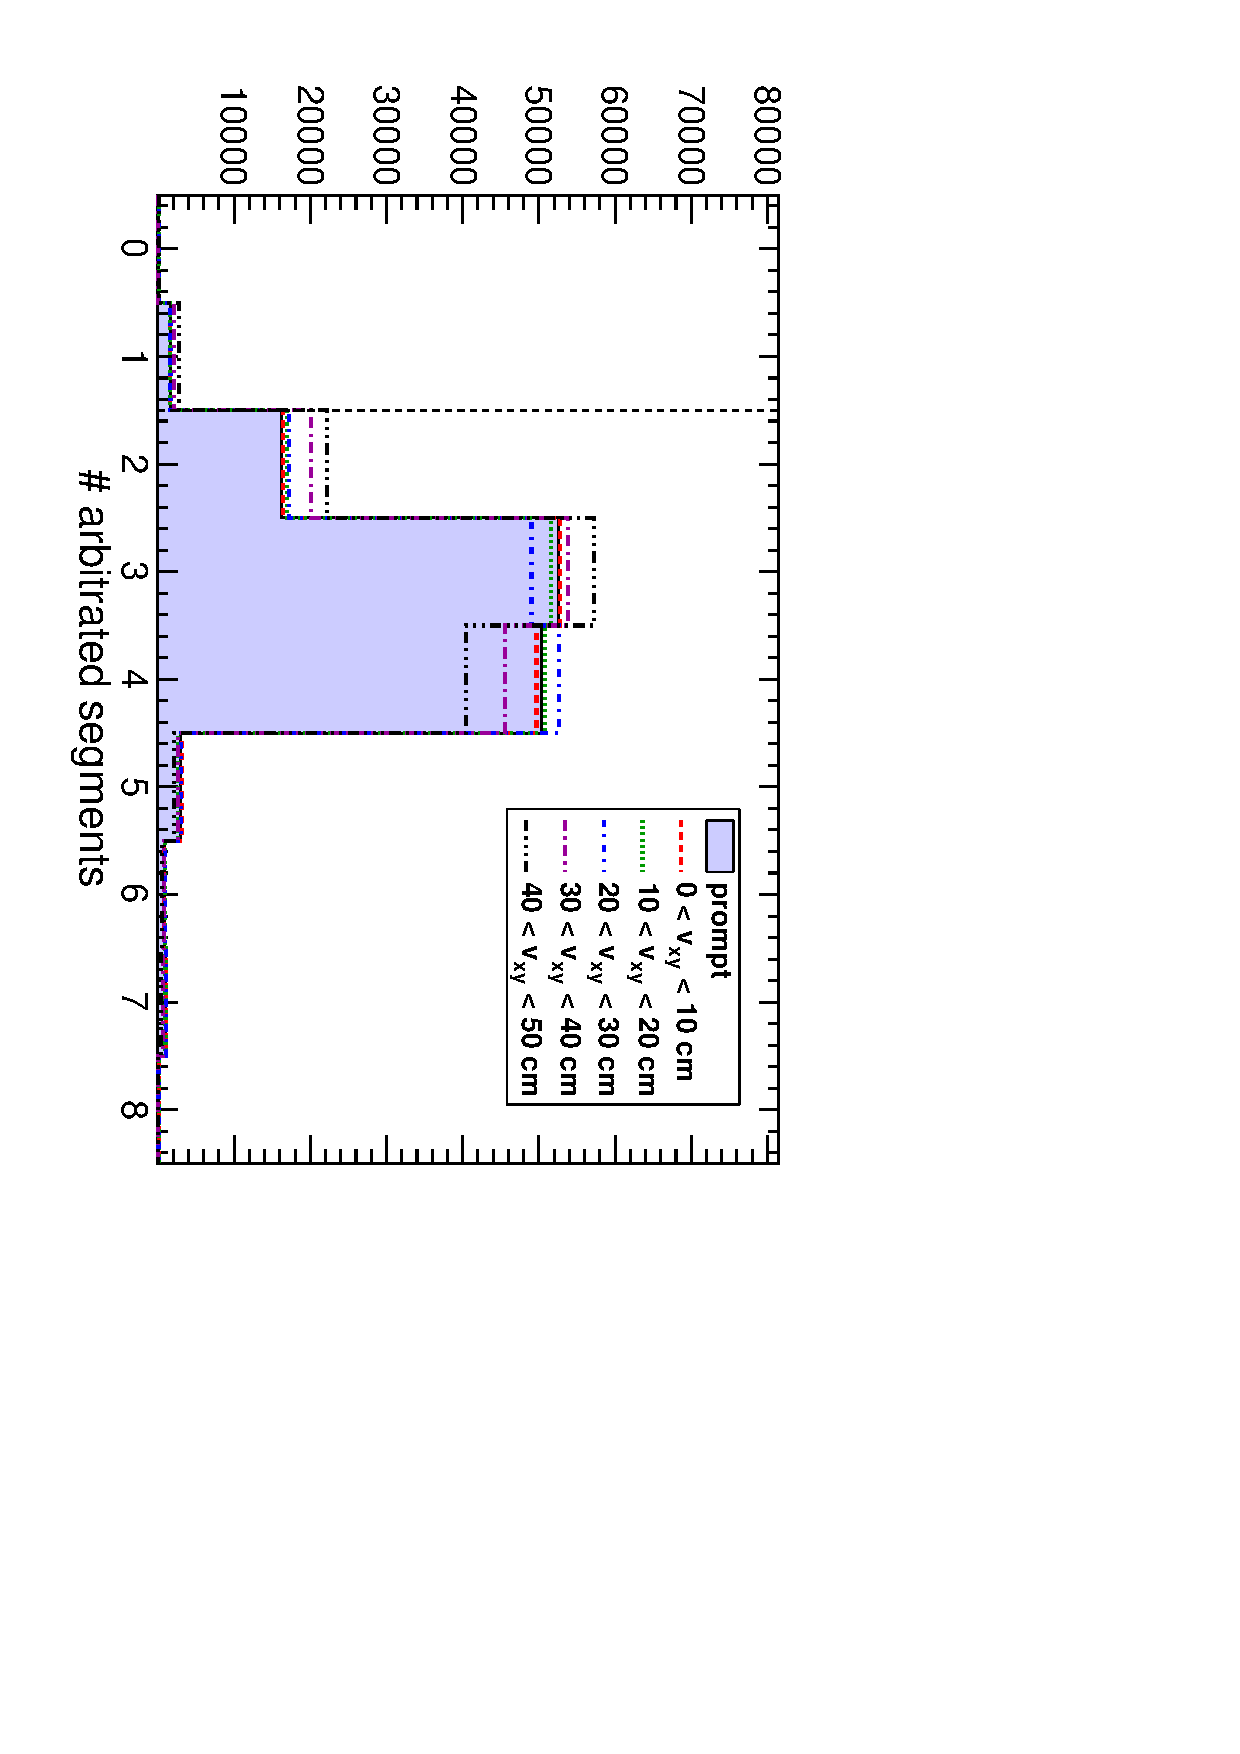
\includegraphics[height=0.49\linewidth, angle=90]{trackslinear_segments.pdf}
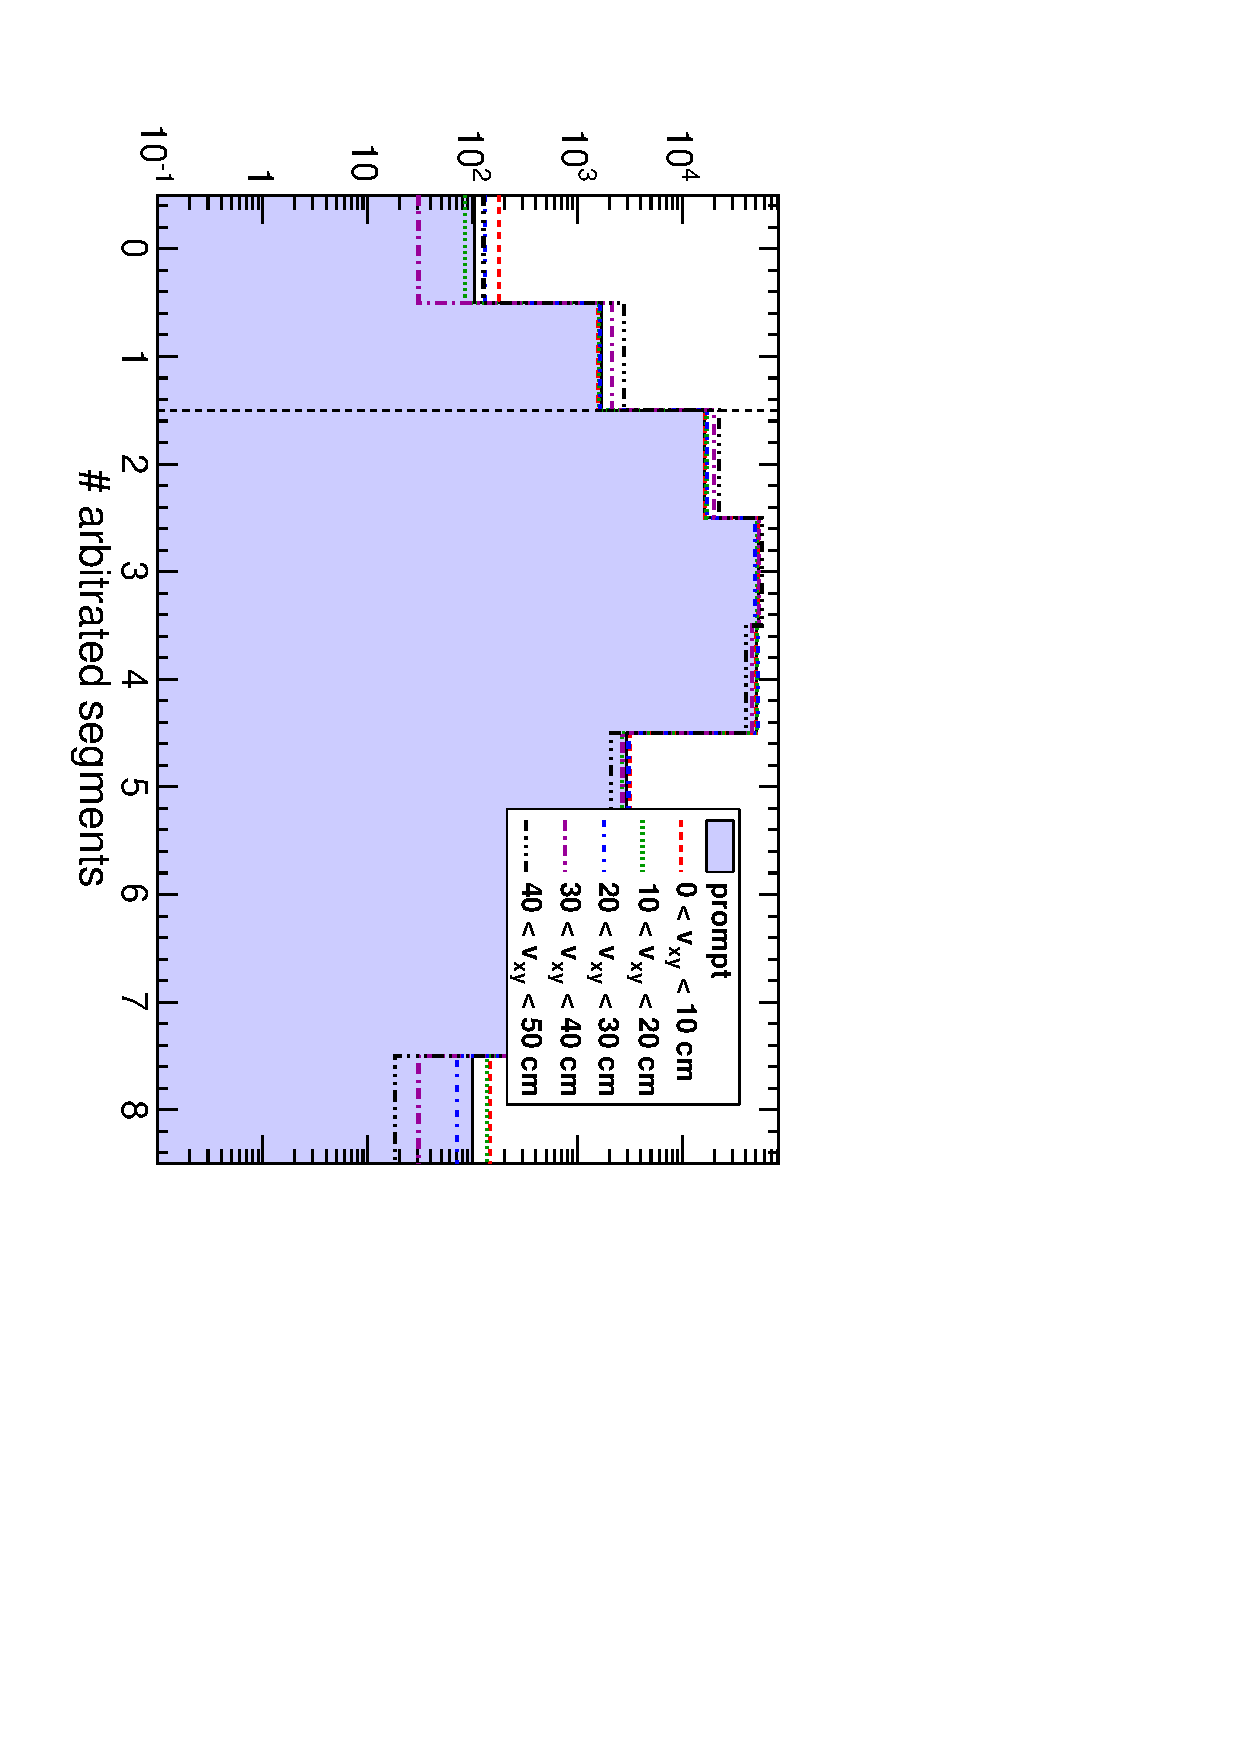
\includegraphics[height=0.49\linewidth, angle=90]{trackslog_segments.pdf}}
\only<2>{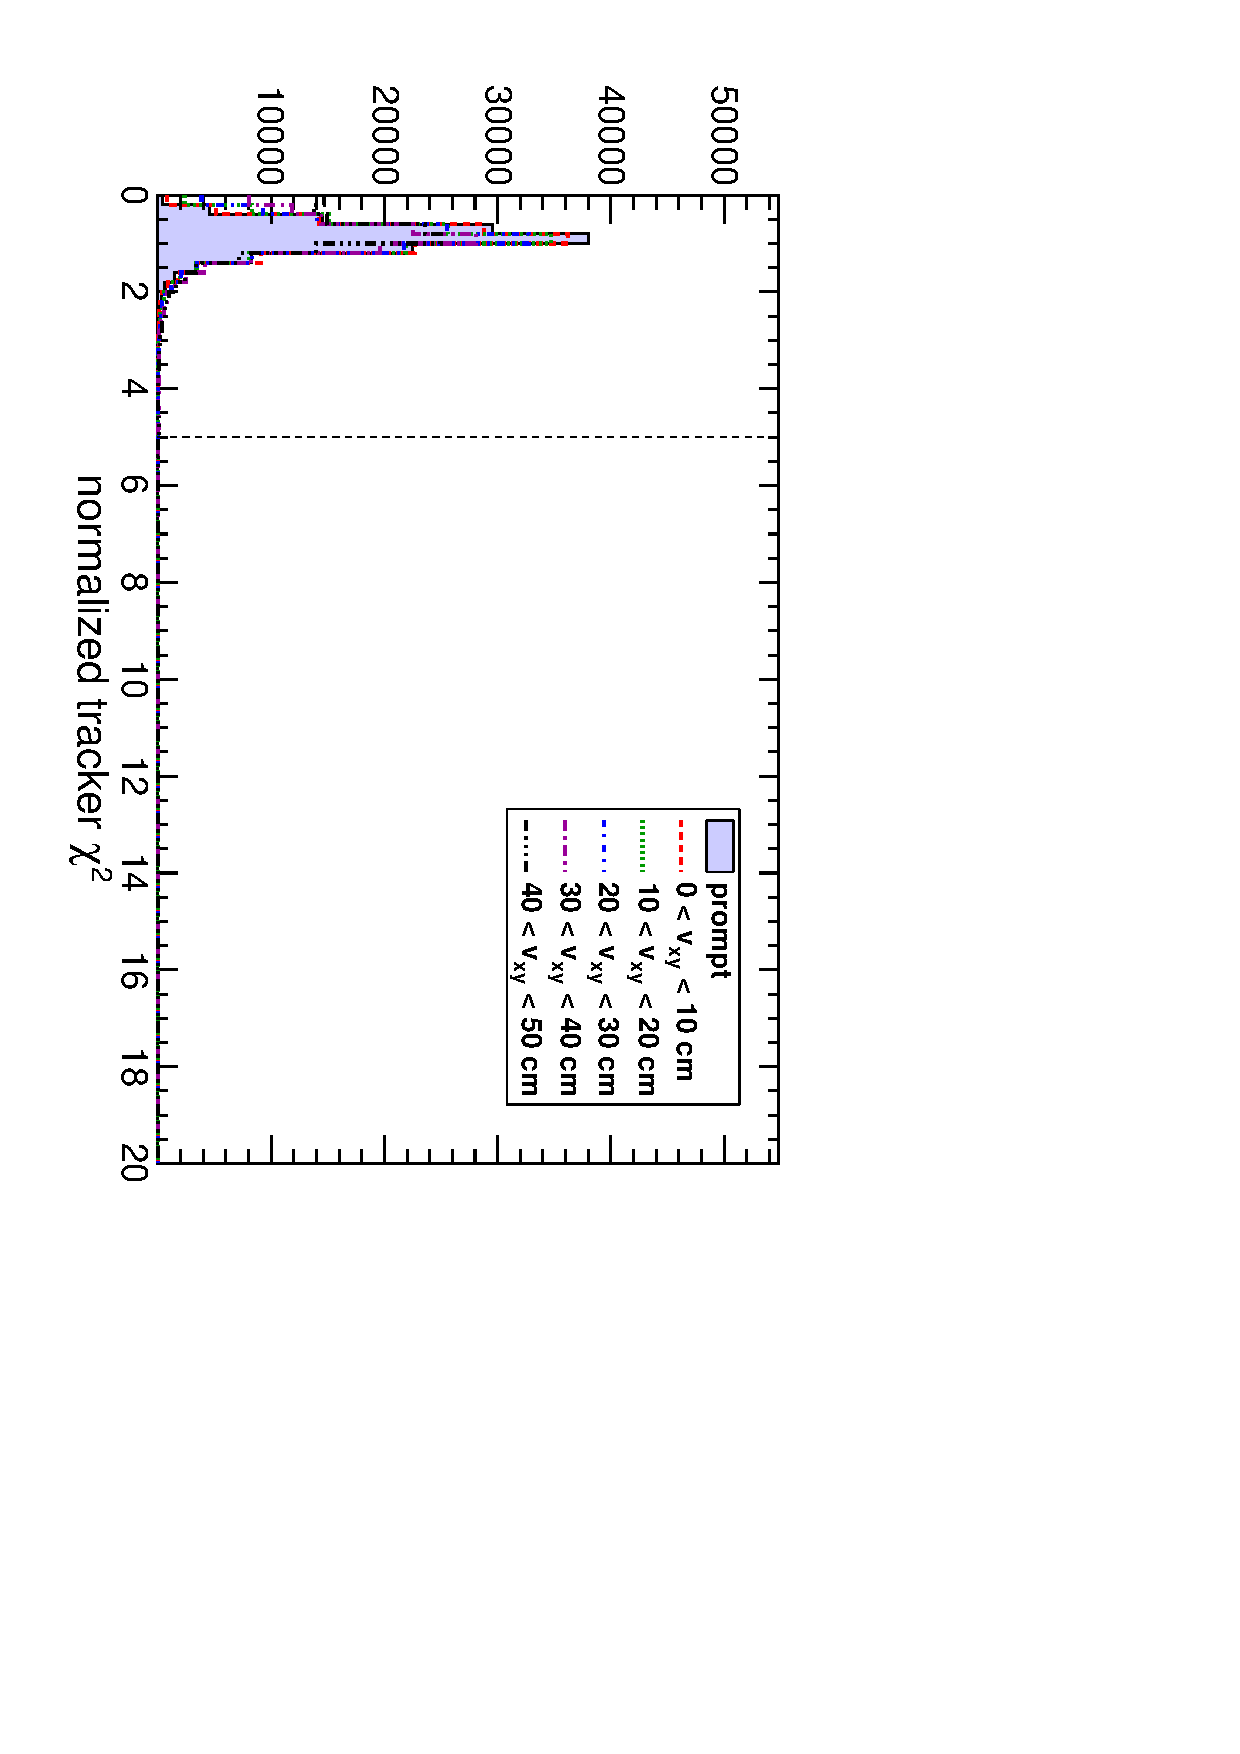
\includegraphics[height=0.49\linewidth, angle=90]{trackslinear_normchi2.pdf}
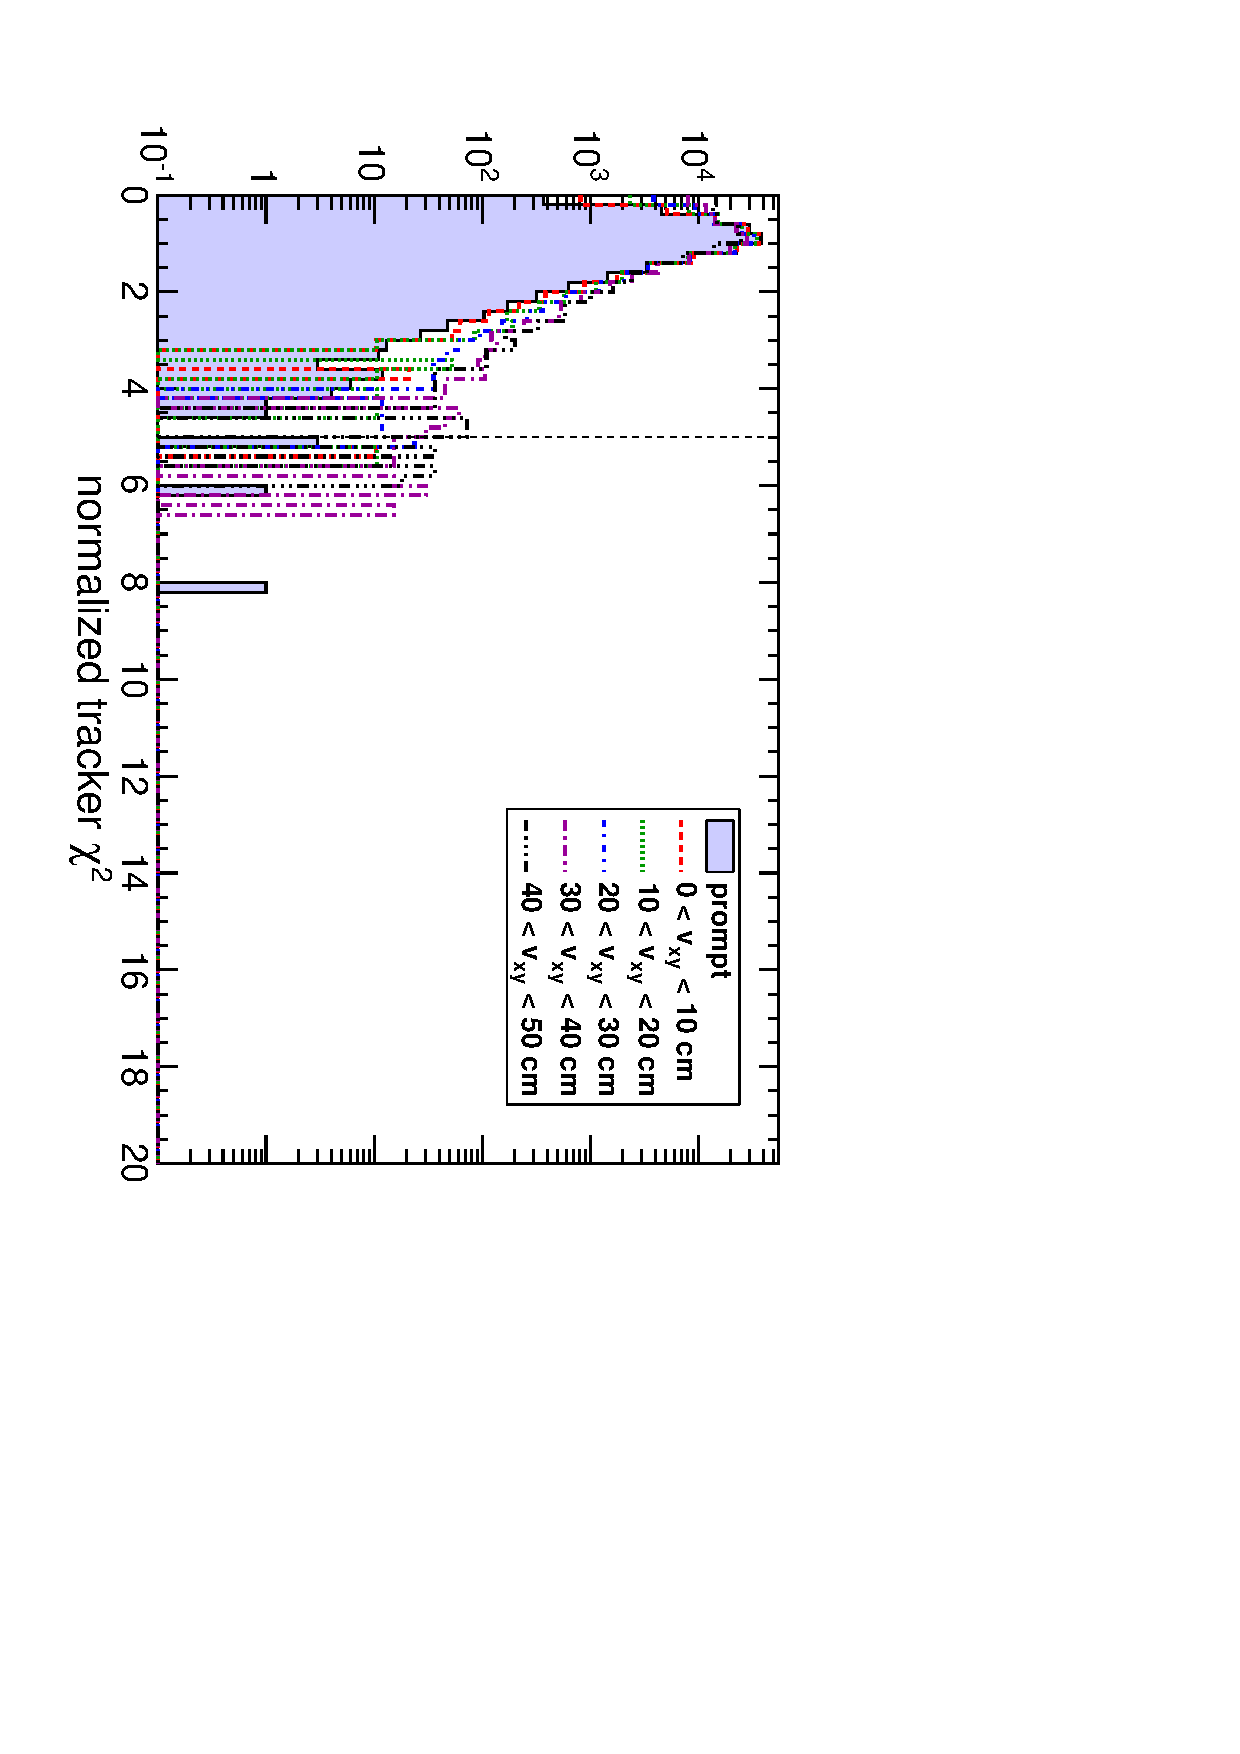
\includegraphics[height=0.49\linewidth, angle=90]{trackslog_normchi2.pdf}}
\only<3>{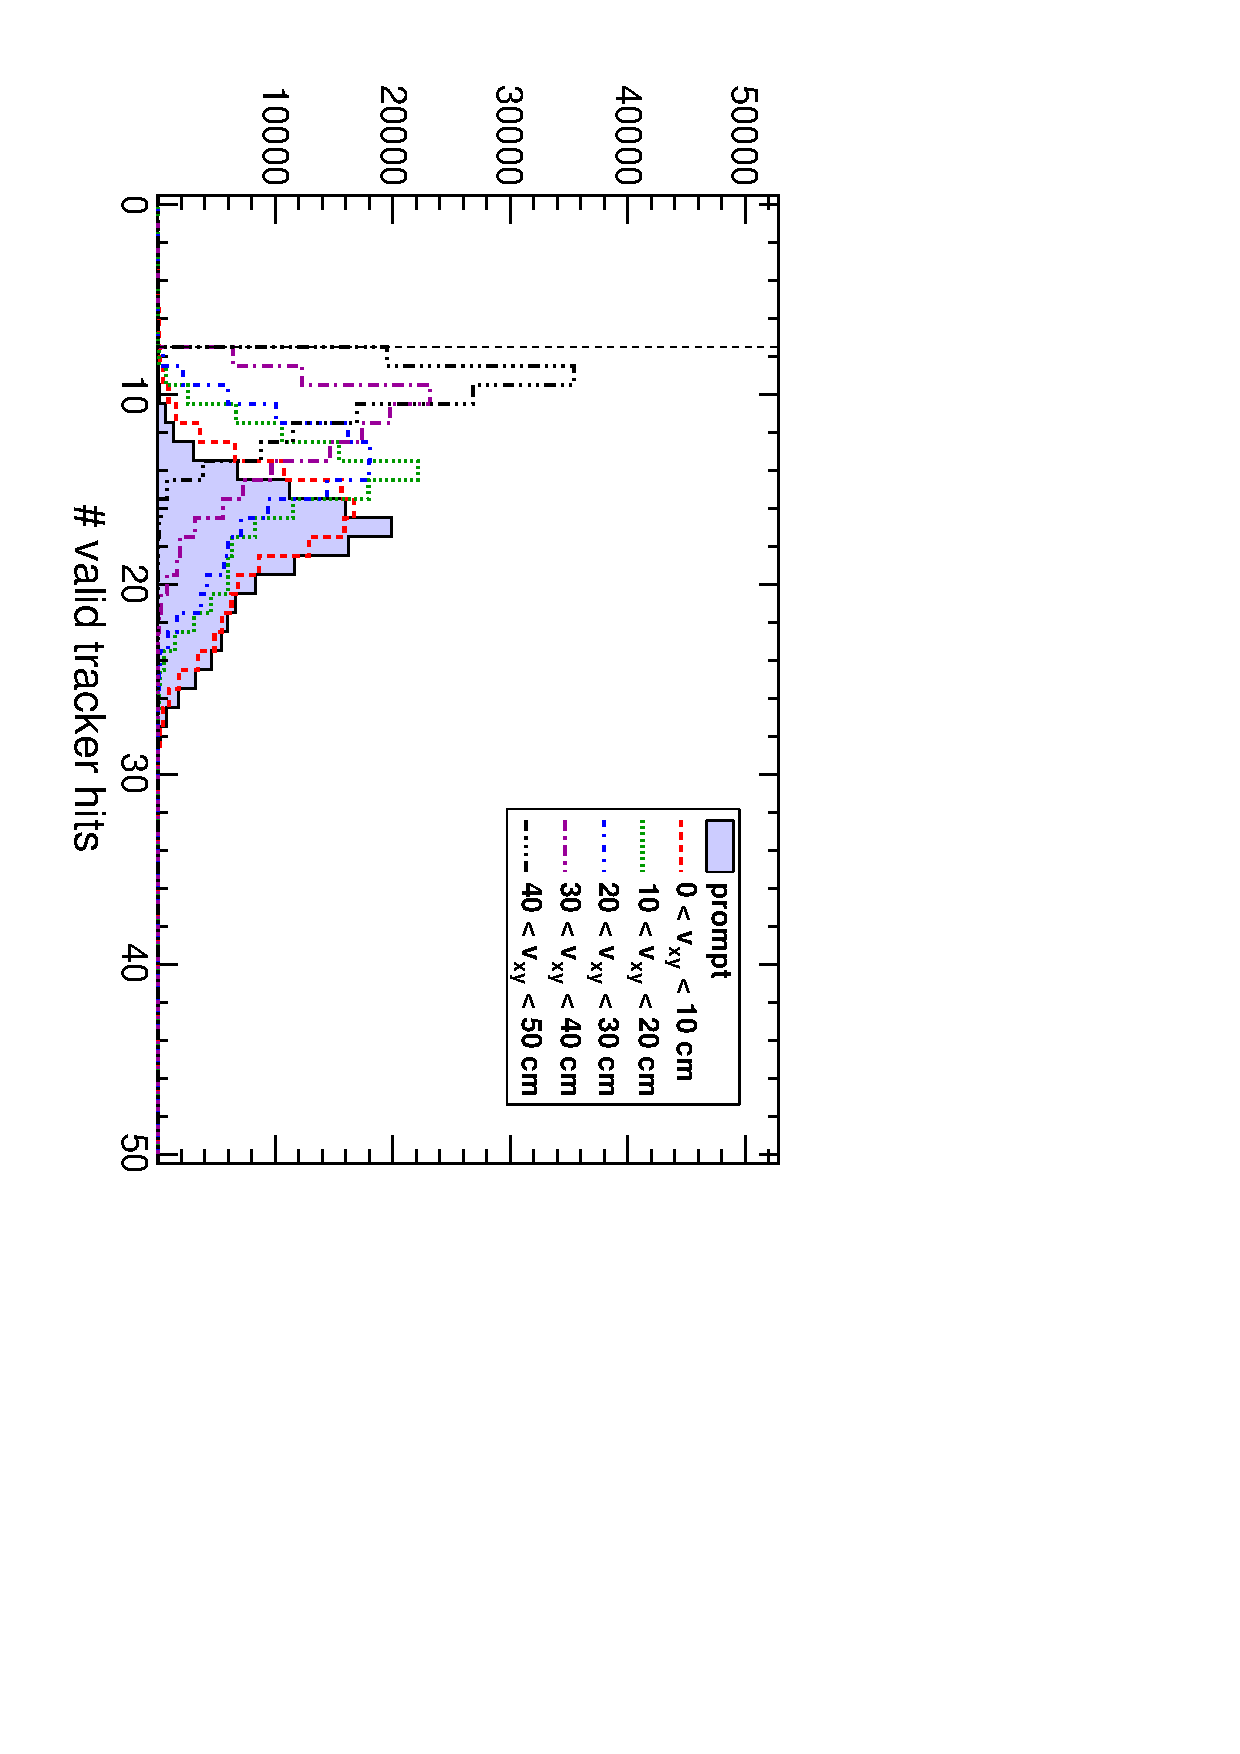
\includegraphics[height=0.49\linewidth, angle=90]{trackslinear_tkhits.pdf}
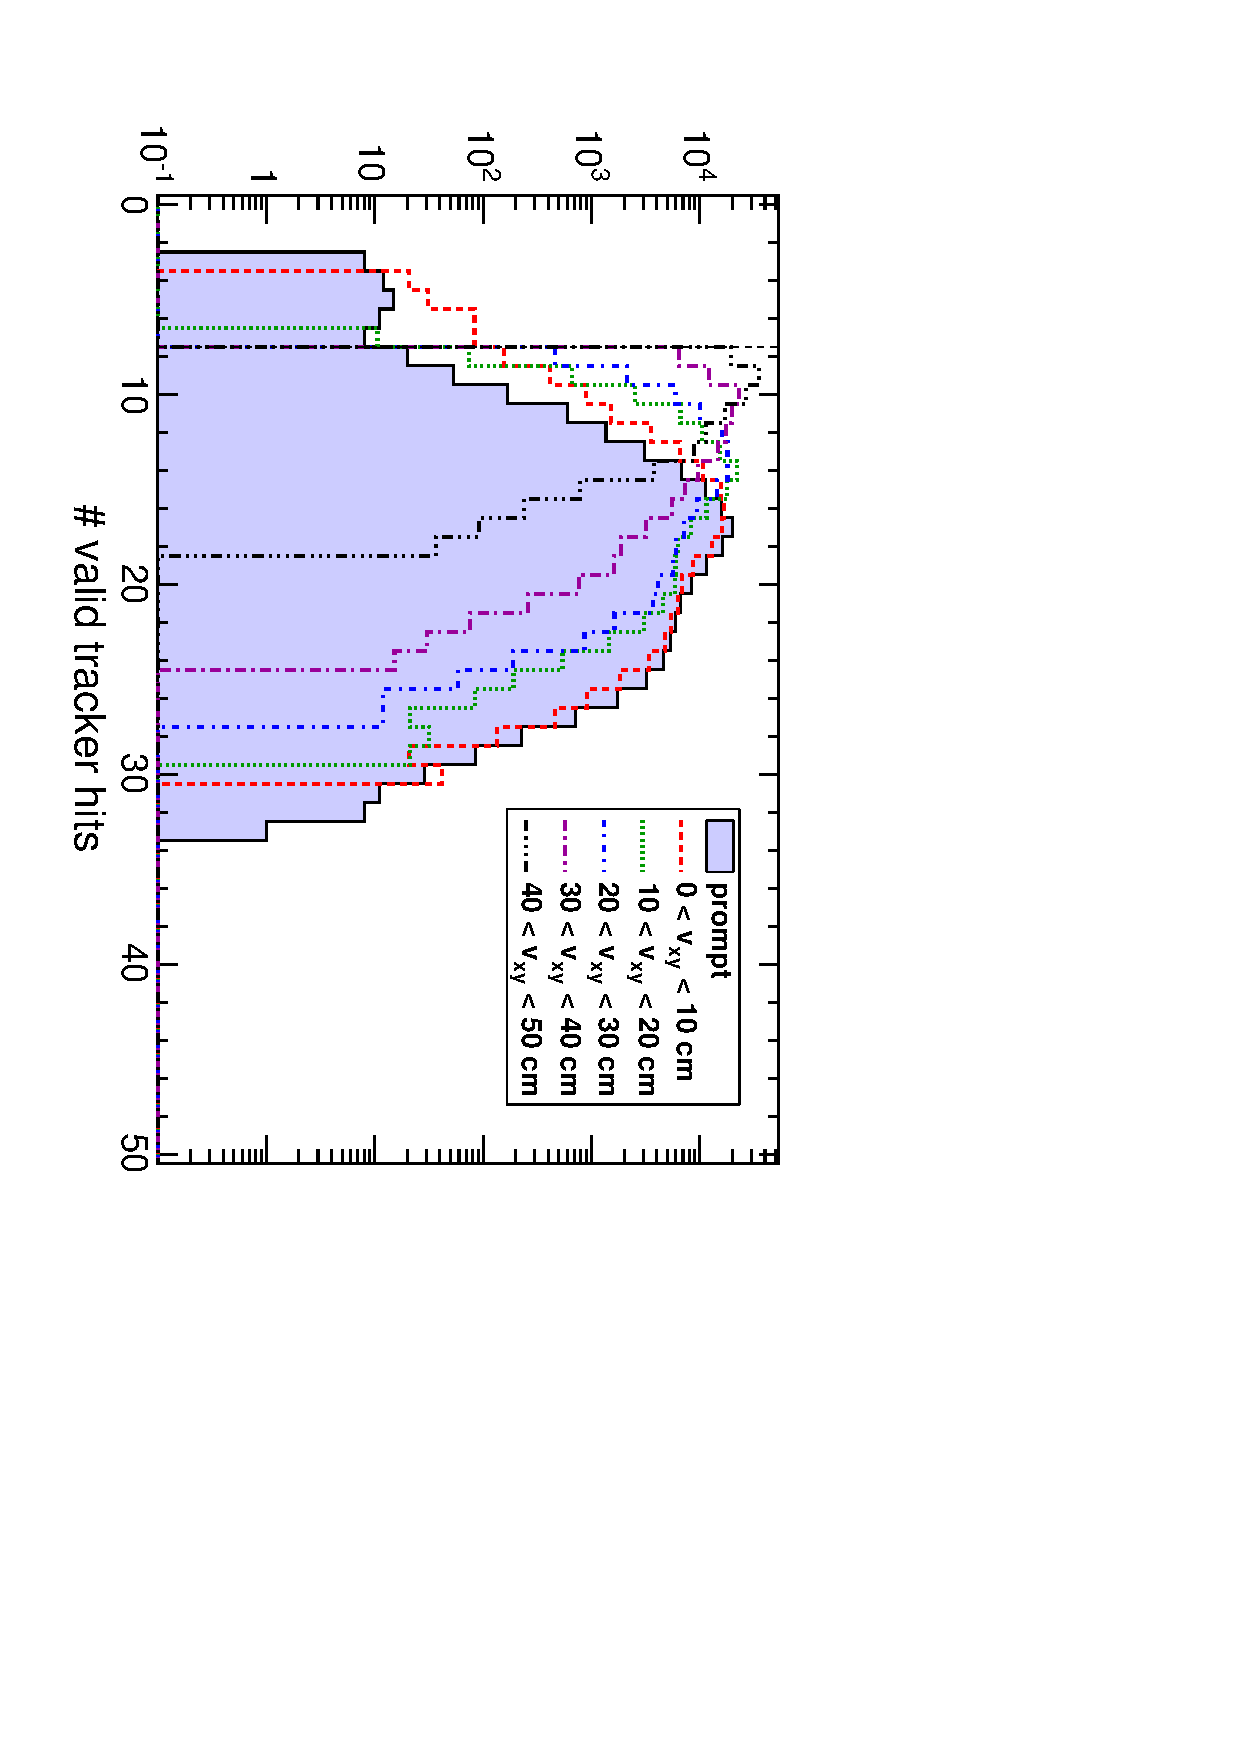
\includegraphics[height=0.49\linewidth, angle=90]{trackslog_tkhits.pdf}}
\only<4>{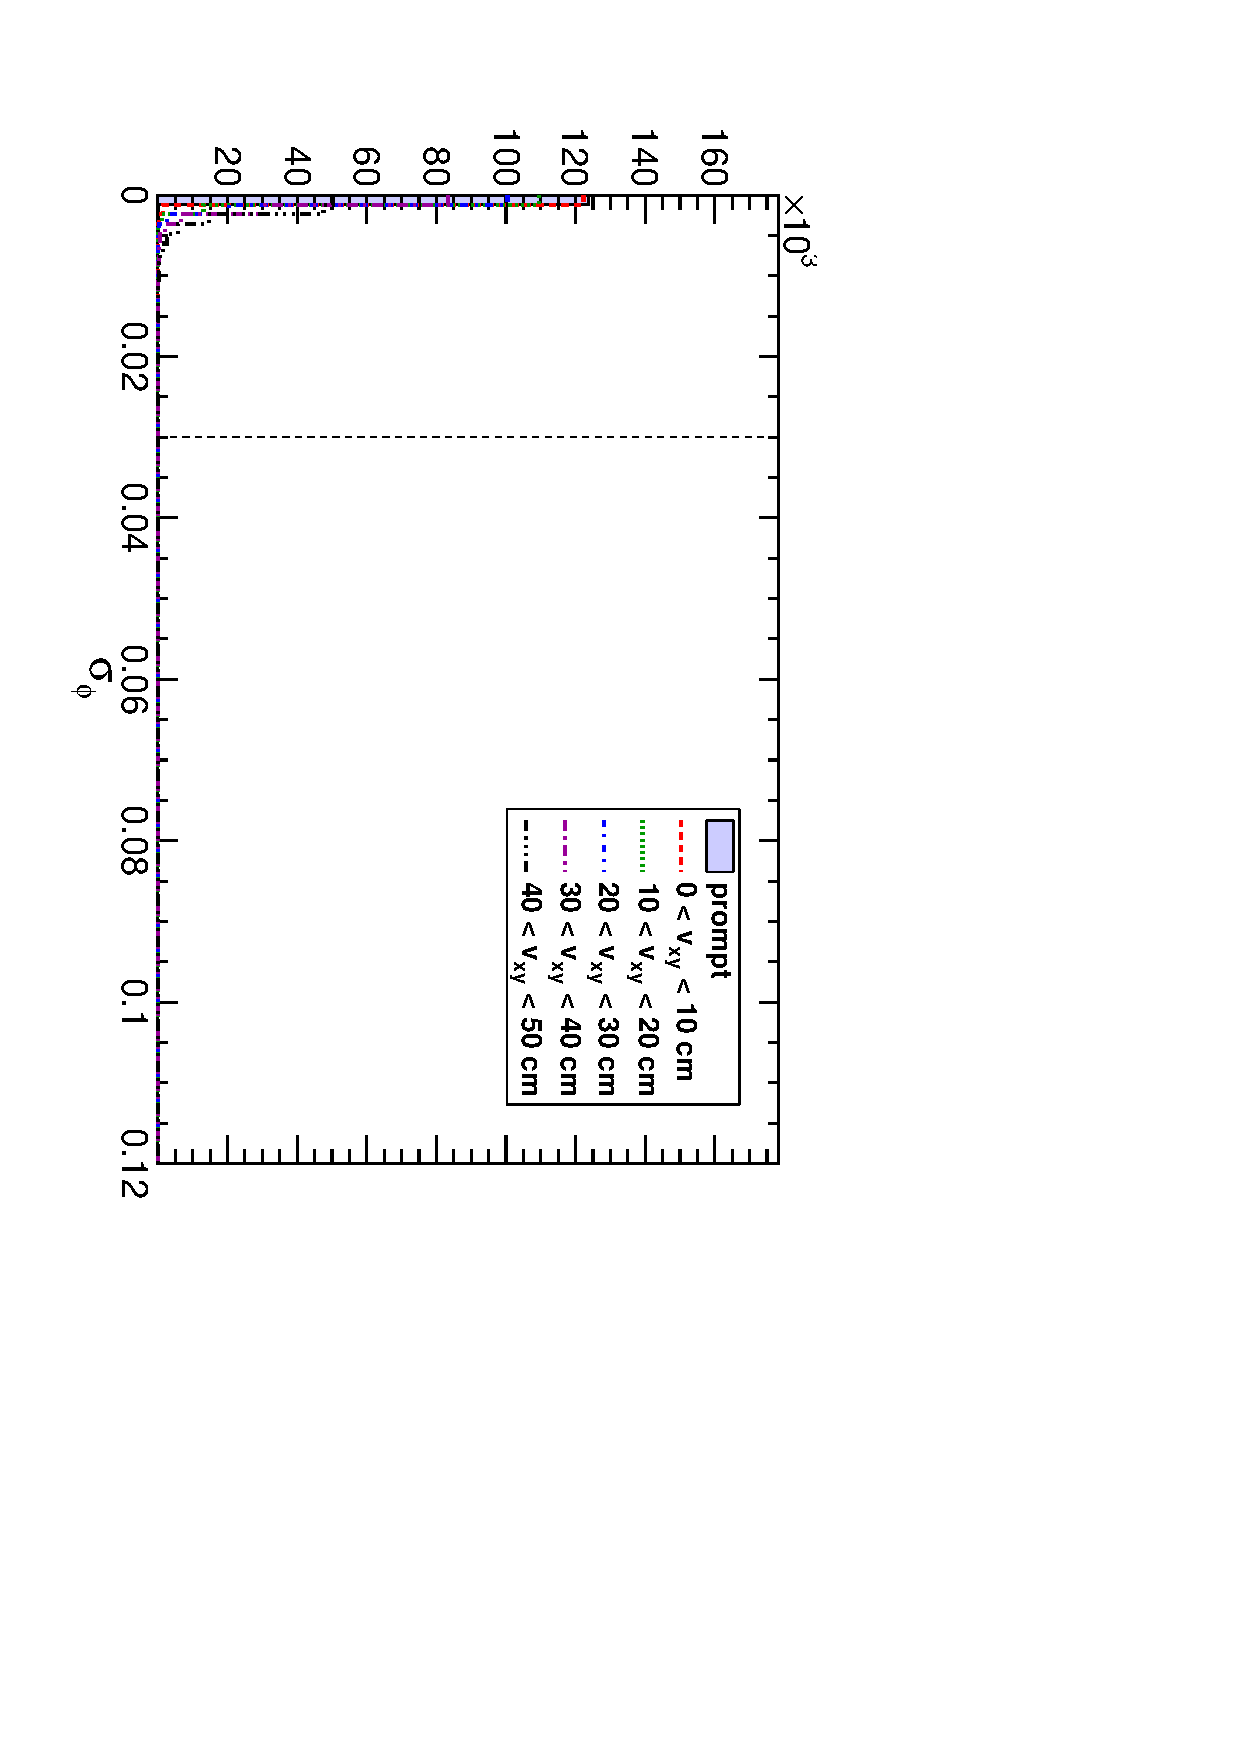
\includegraphics[height=0.49\linewidth, angle=90]{trackslinear_phierr.pdf}
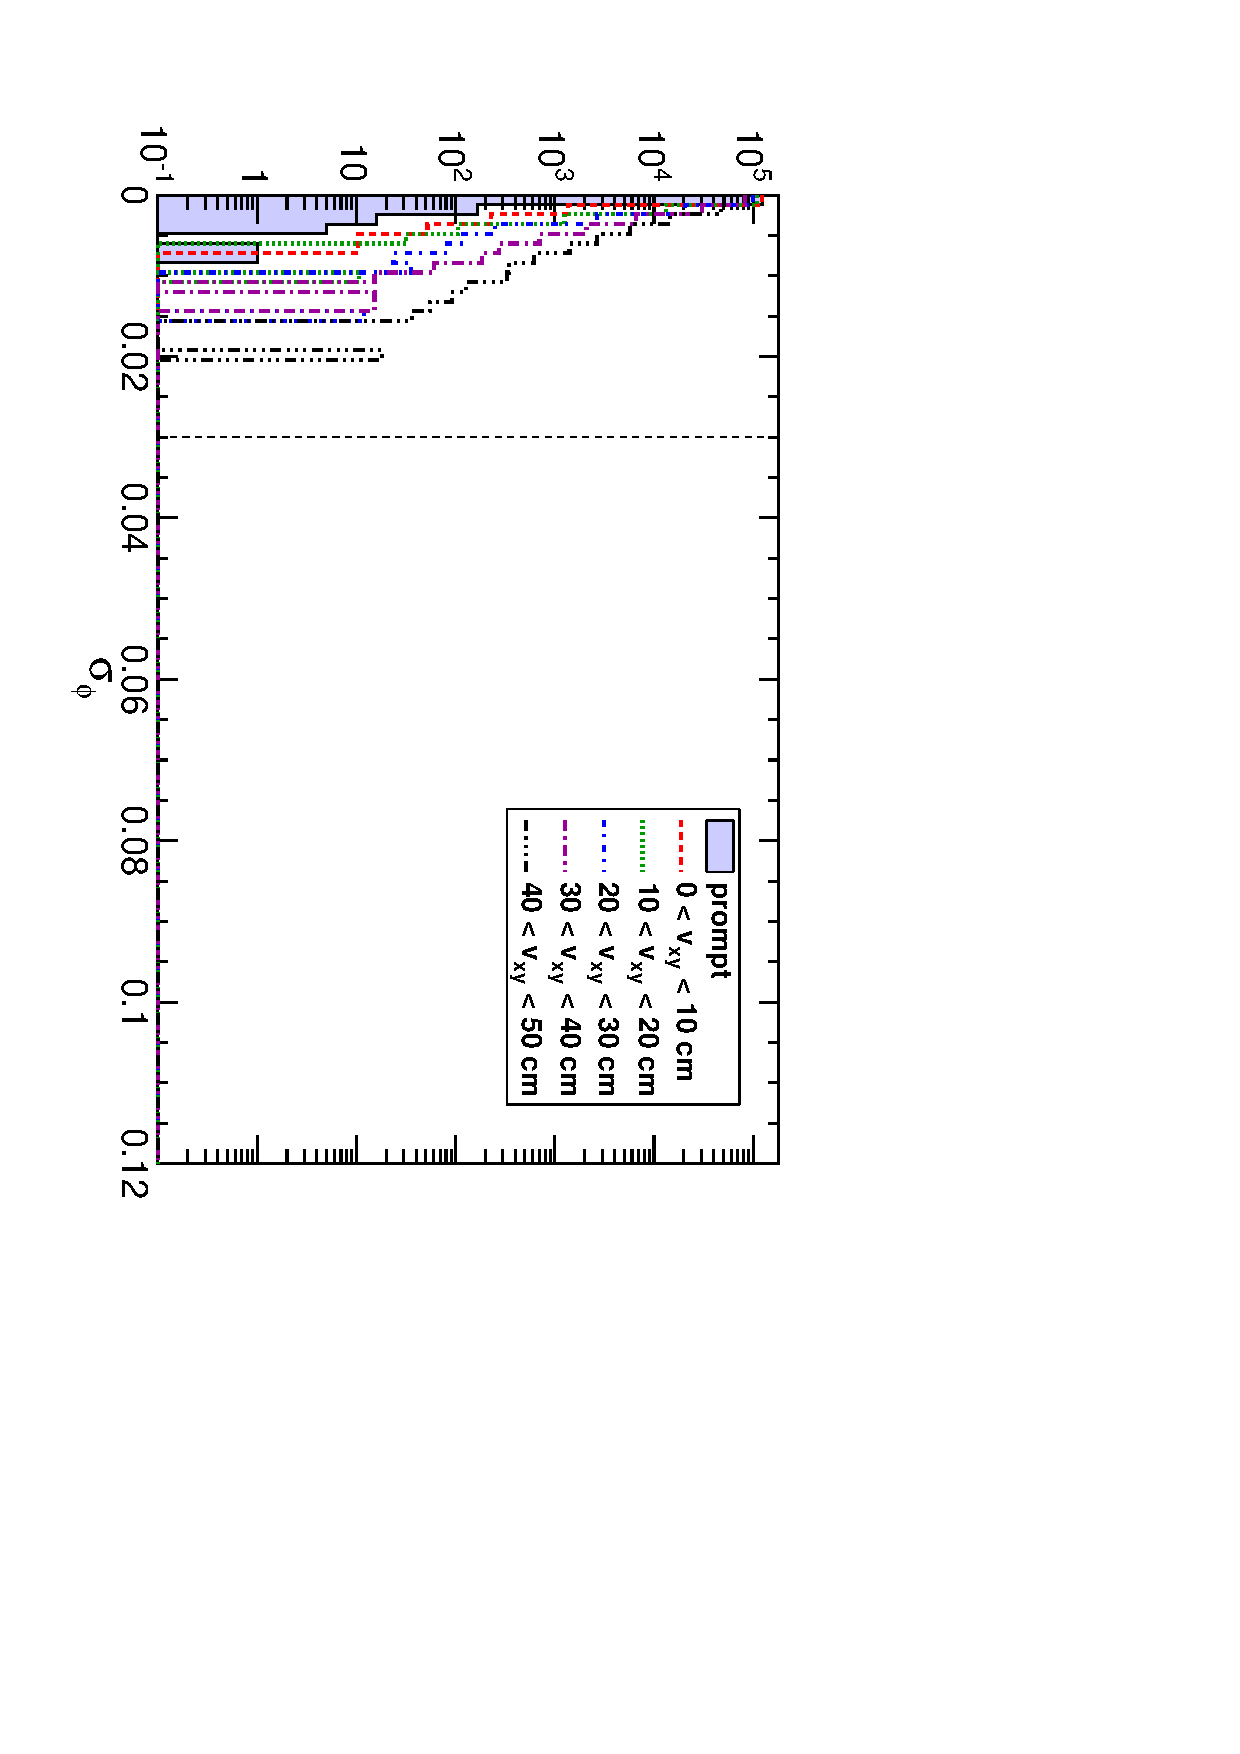
\includegraphics[height=0.49\linewidth, angle=90]{trackslog_phierr.pdf}}
\only<5>{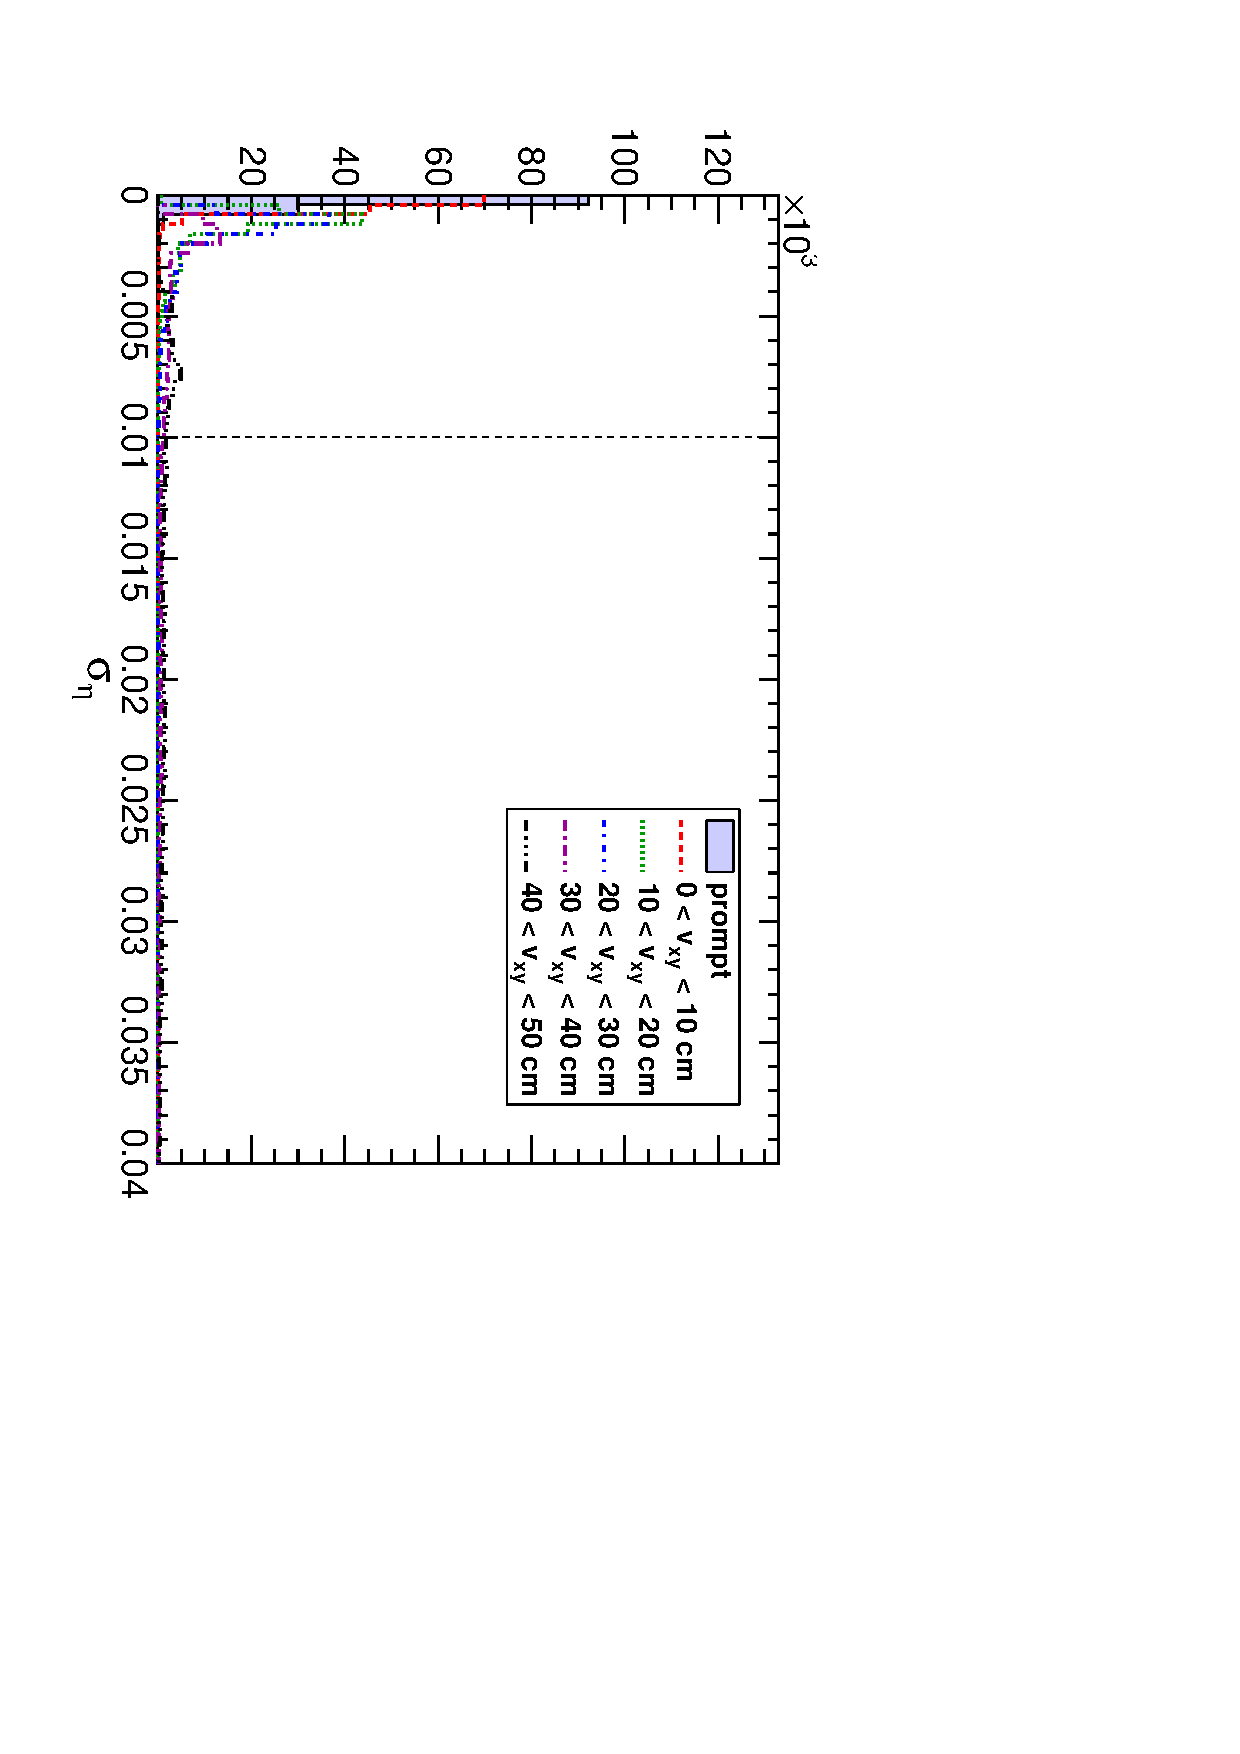
\includegraphics[height=0.49\linewidth, angle=90]{trackslinear_etaerr.pdf}
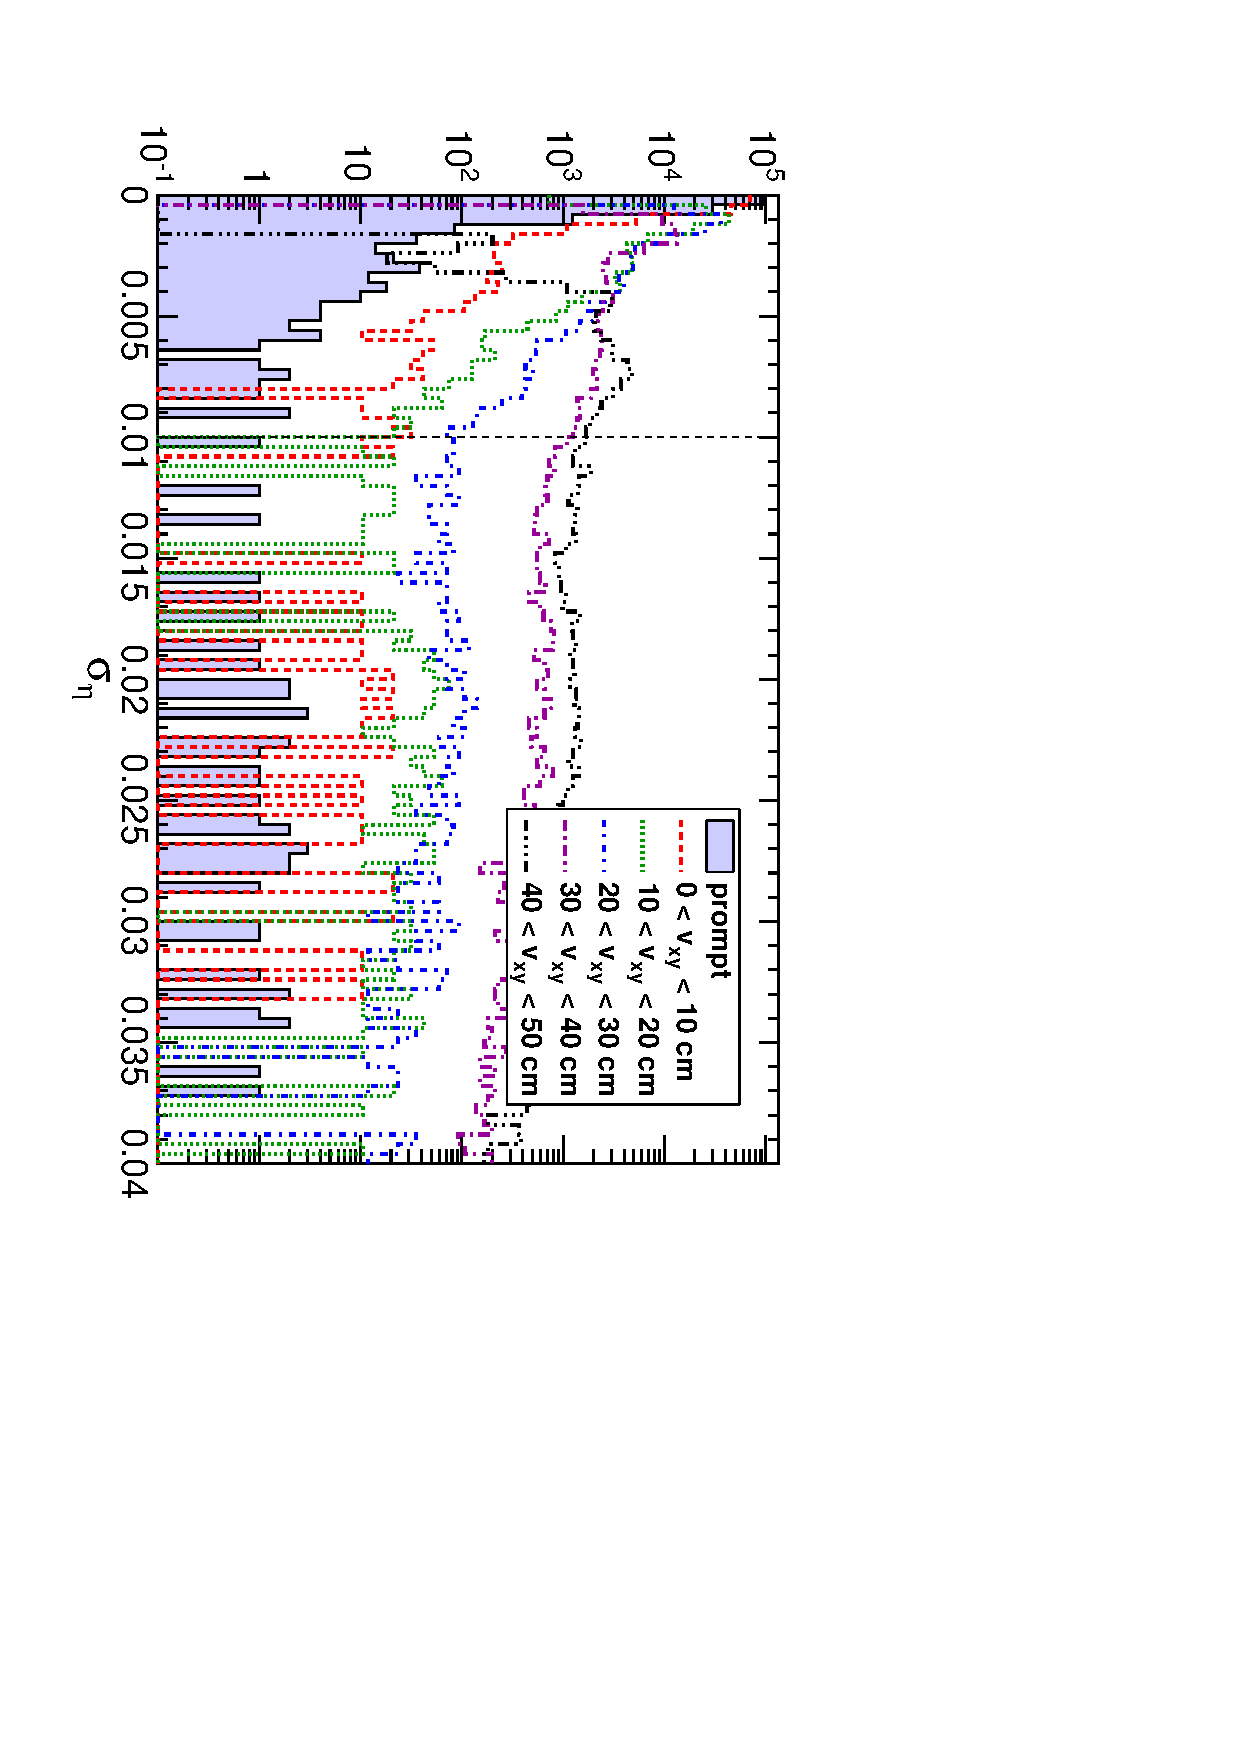
\includegraphics[height=0.49\linewidth, angle=90]{trackslog_etaerr.pdf}}
\only<6>{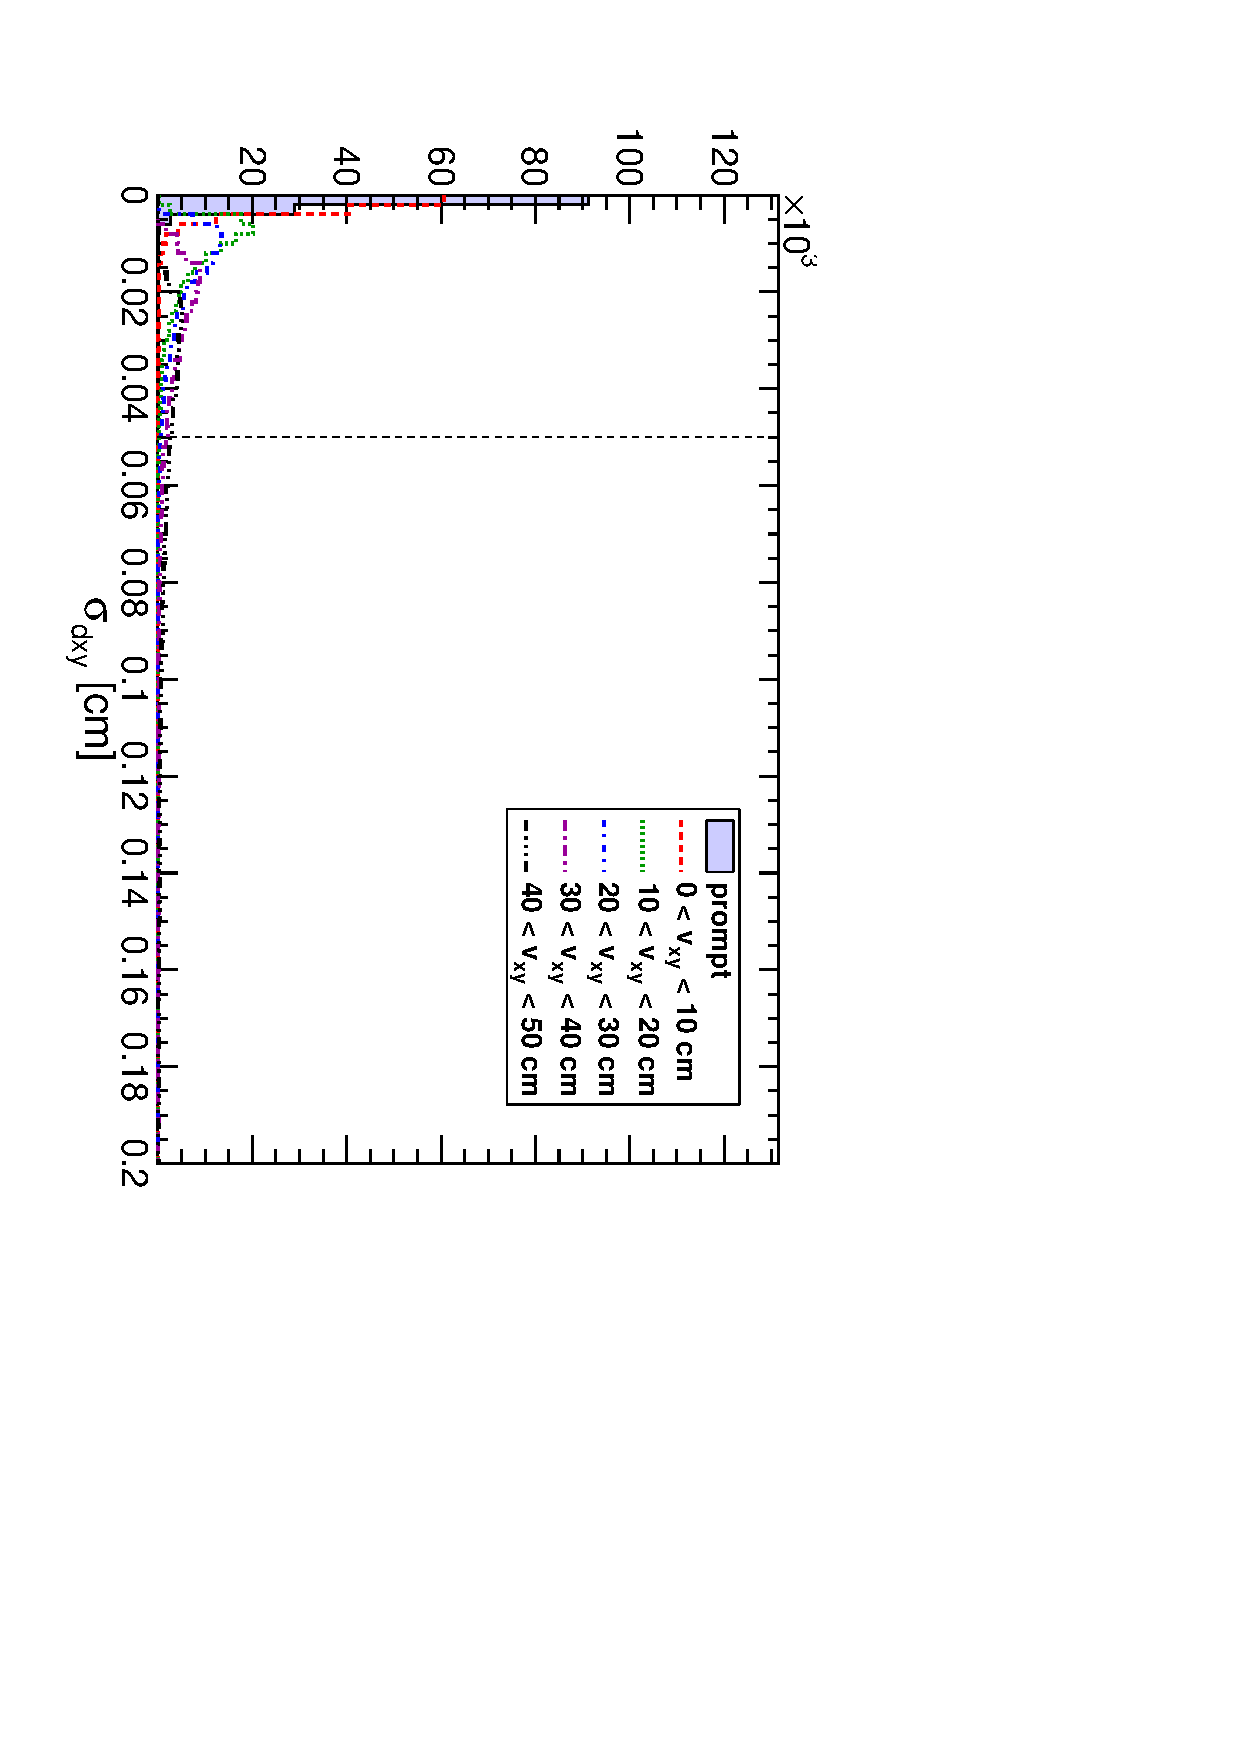
\includegraphics[height=0.49\linewidth, angle=90]{trackslinear_dxyerr.pdf}
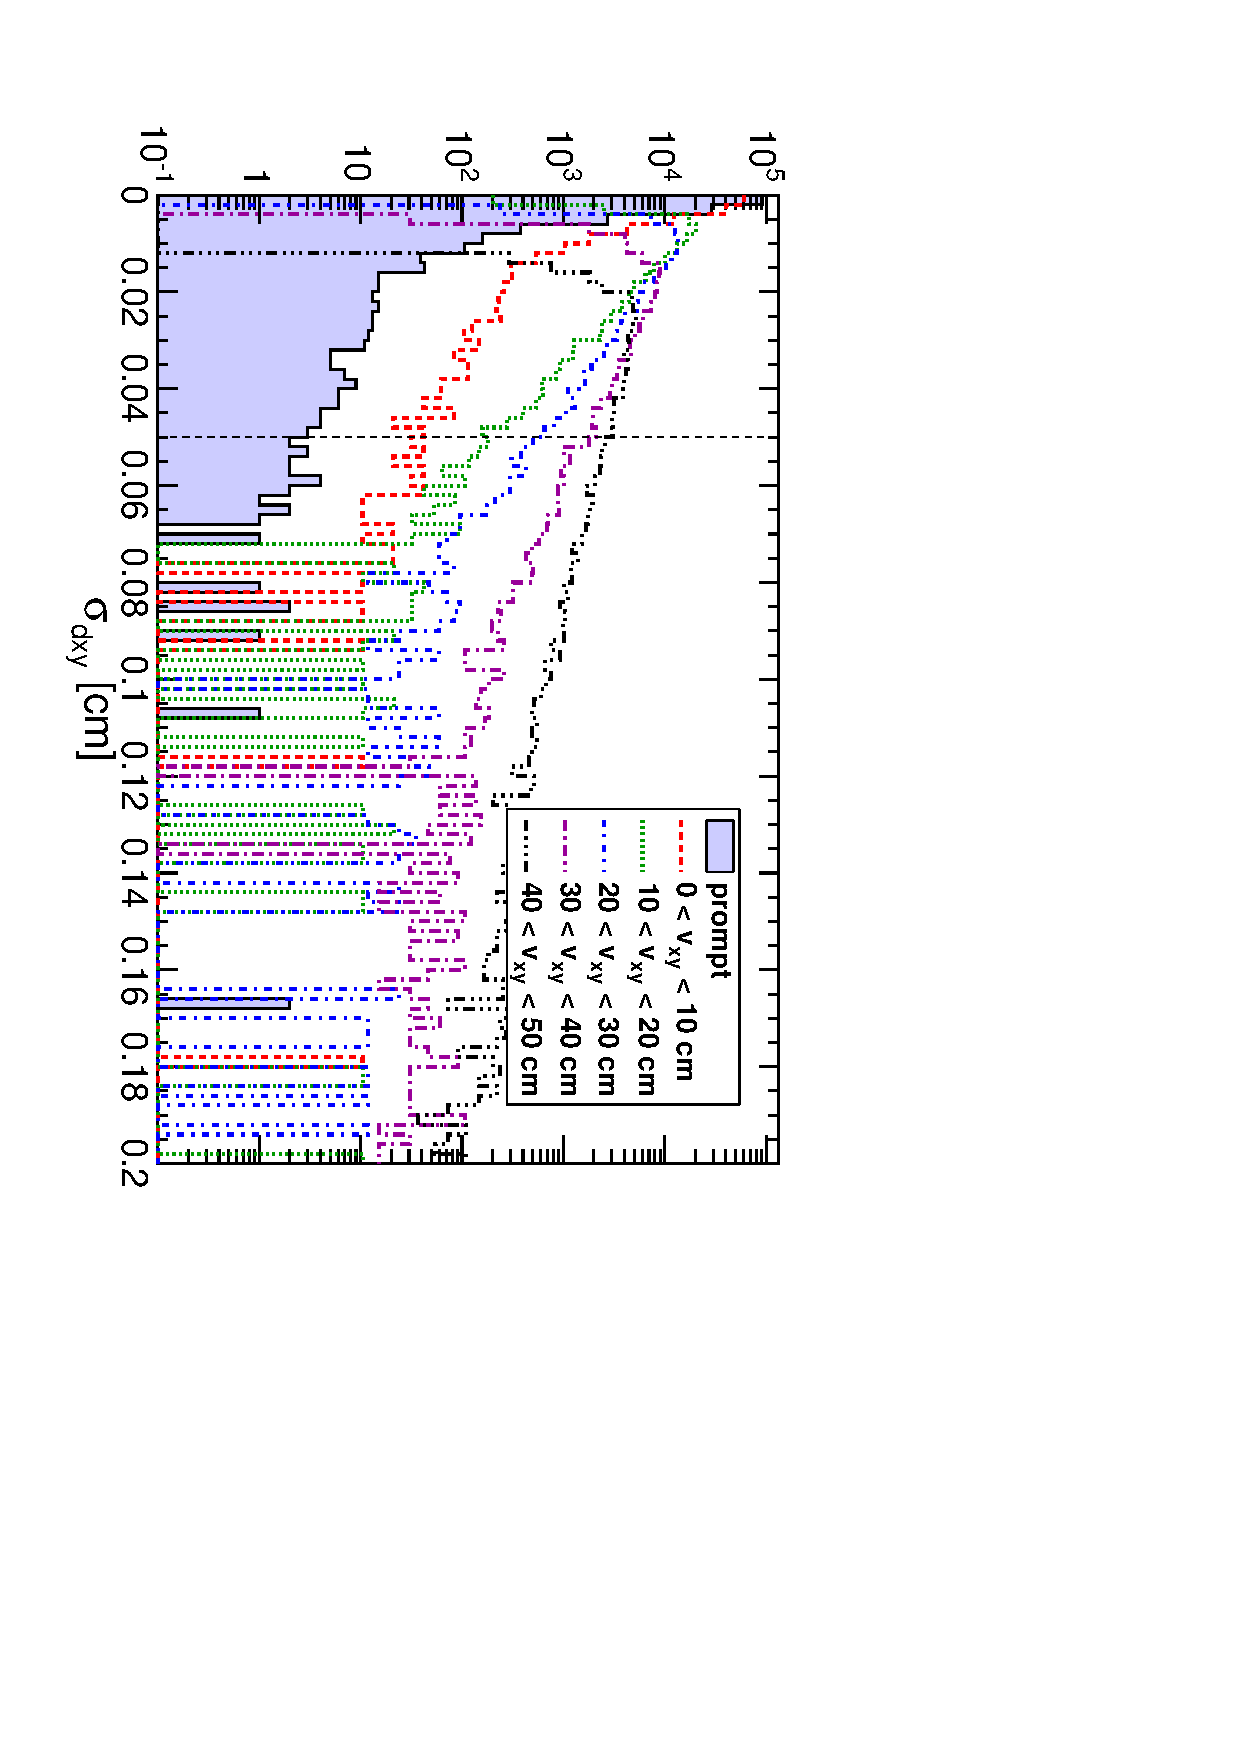
\includegraphics[height=0.49\linewidth, angle=90]{trackslog_dxyerr.pdf}}
\only<7>{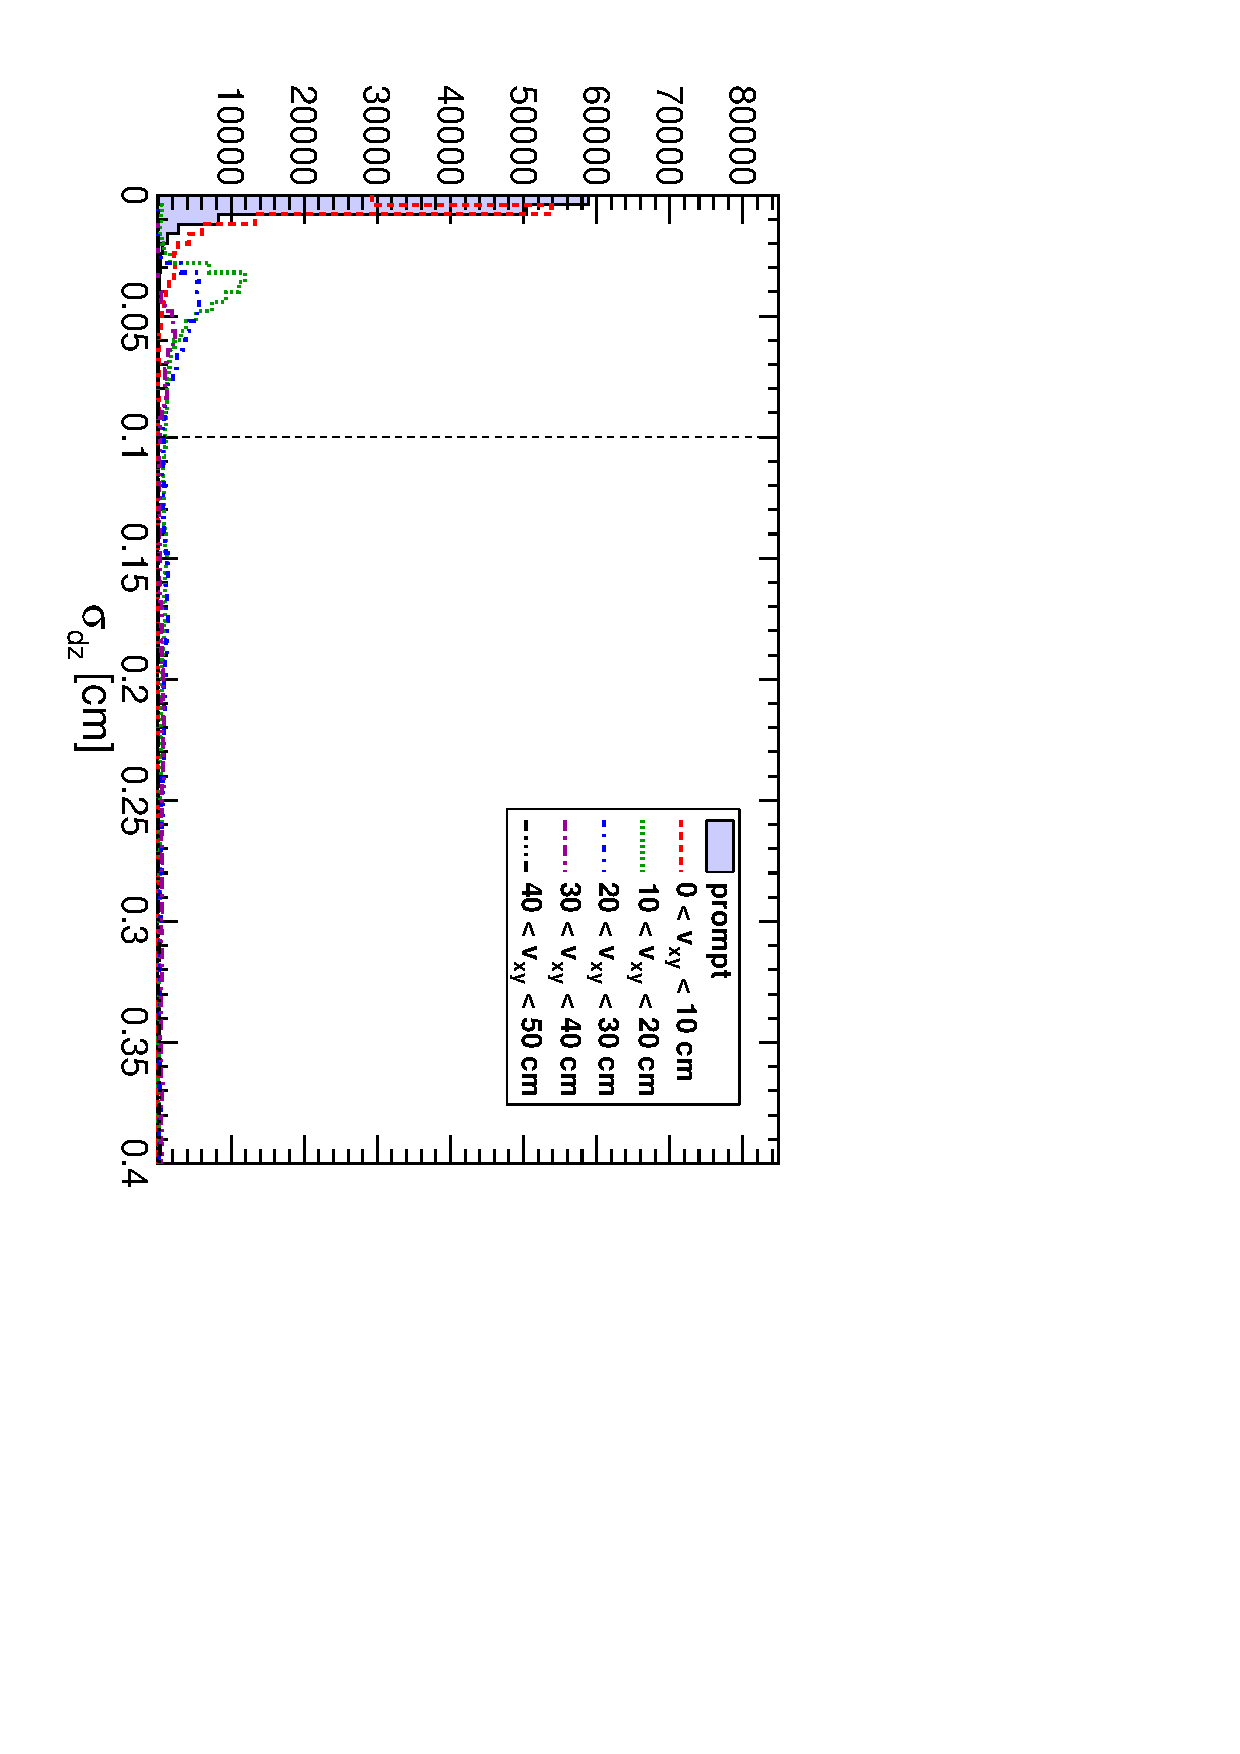
\includegraphics[height=0.49\linewidth, angle=90]{trackslinear_dzerr.pdf}
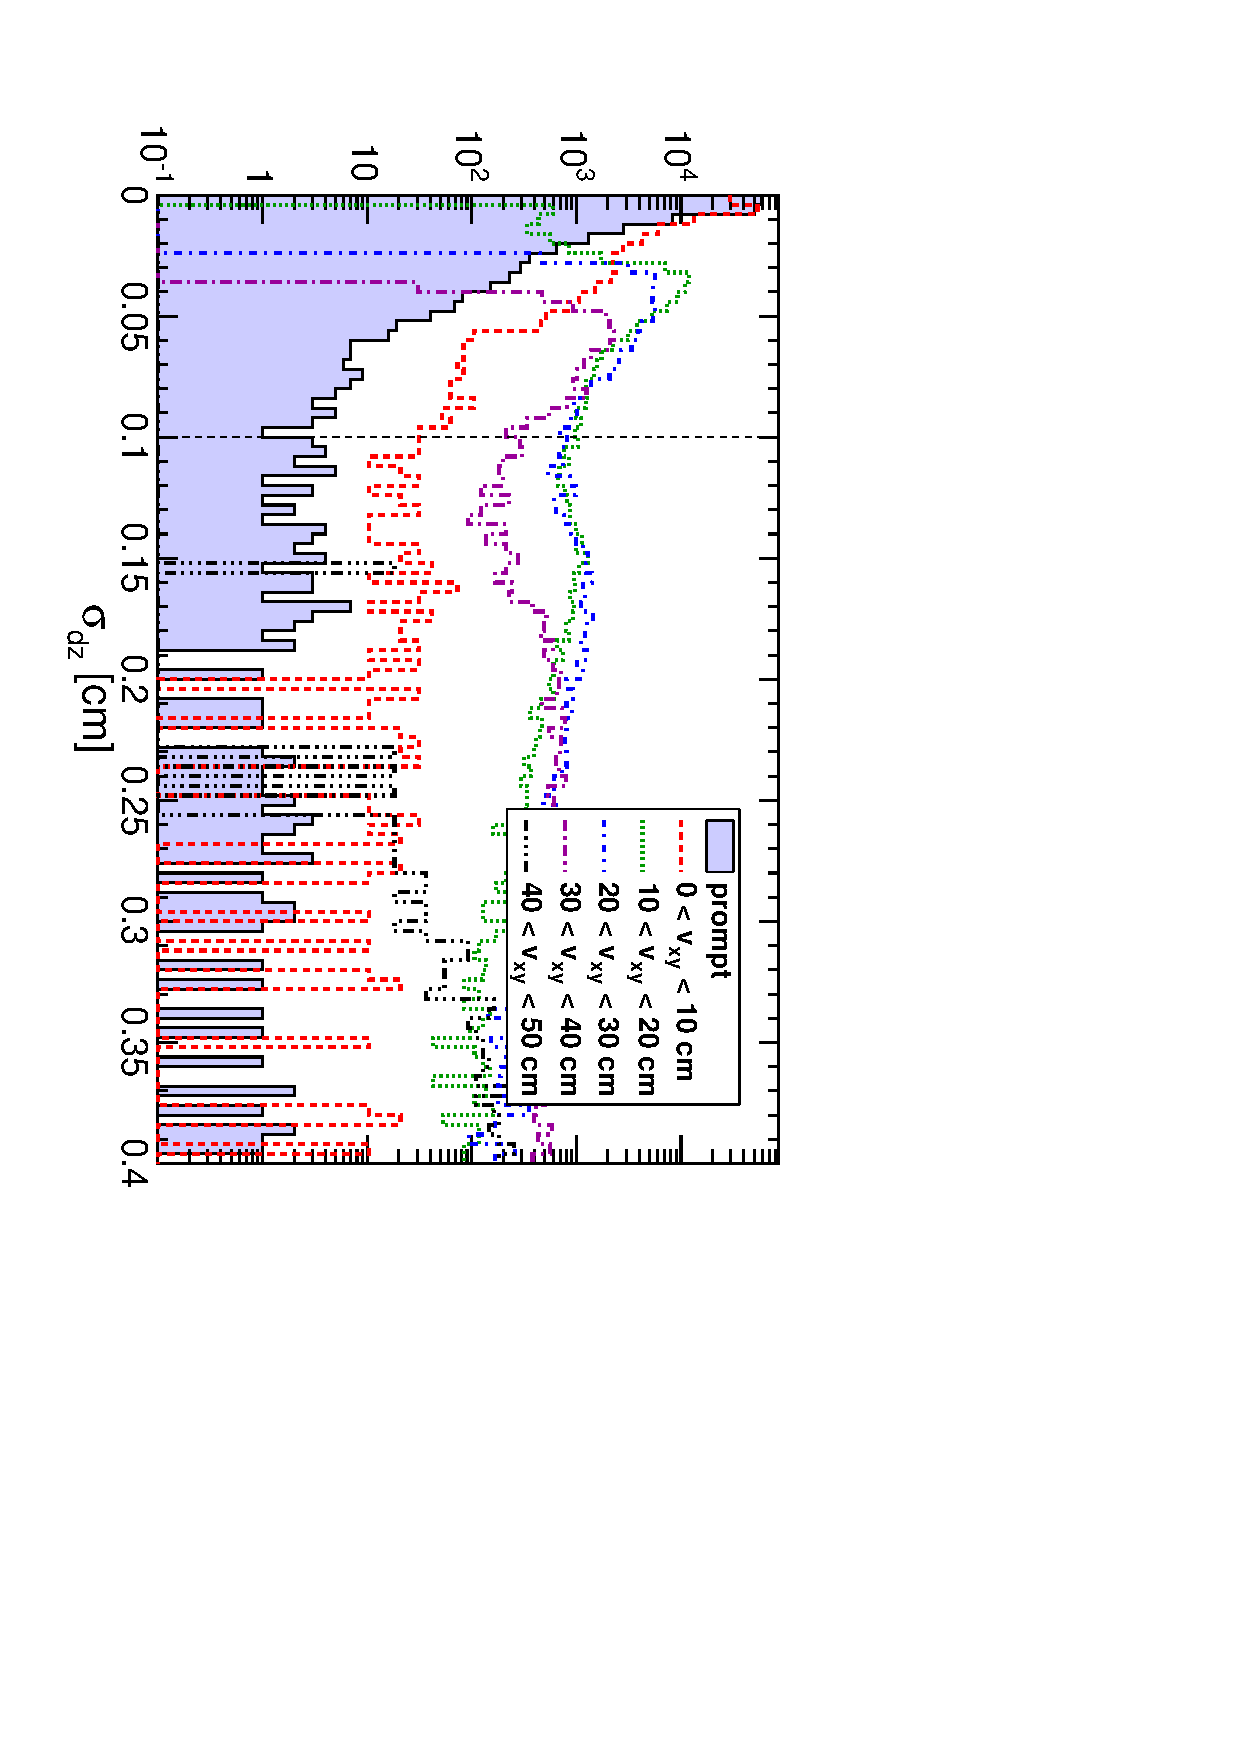
\includegraphics[height=0.49\linewidth, angle=90]{trackslog_dzerr.pdf}}
\end{frame}

\begin{frame}
\frametitle{One more thing\ldots}

\begin{itemize}
\item The arbitrated segments are not necessarily on different chambers
\item No evidence yet that we can get an improvement by requiring a
  minimum number of segments on different chambers, but we should just
  keep it in mind
\end{itemize}

\begin{center}
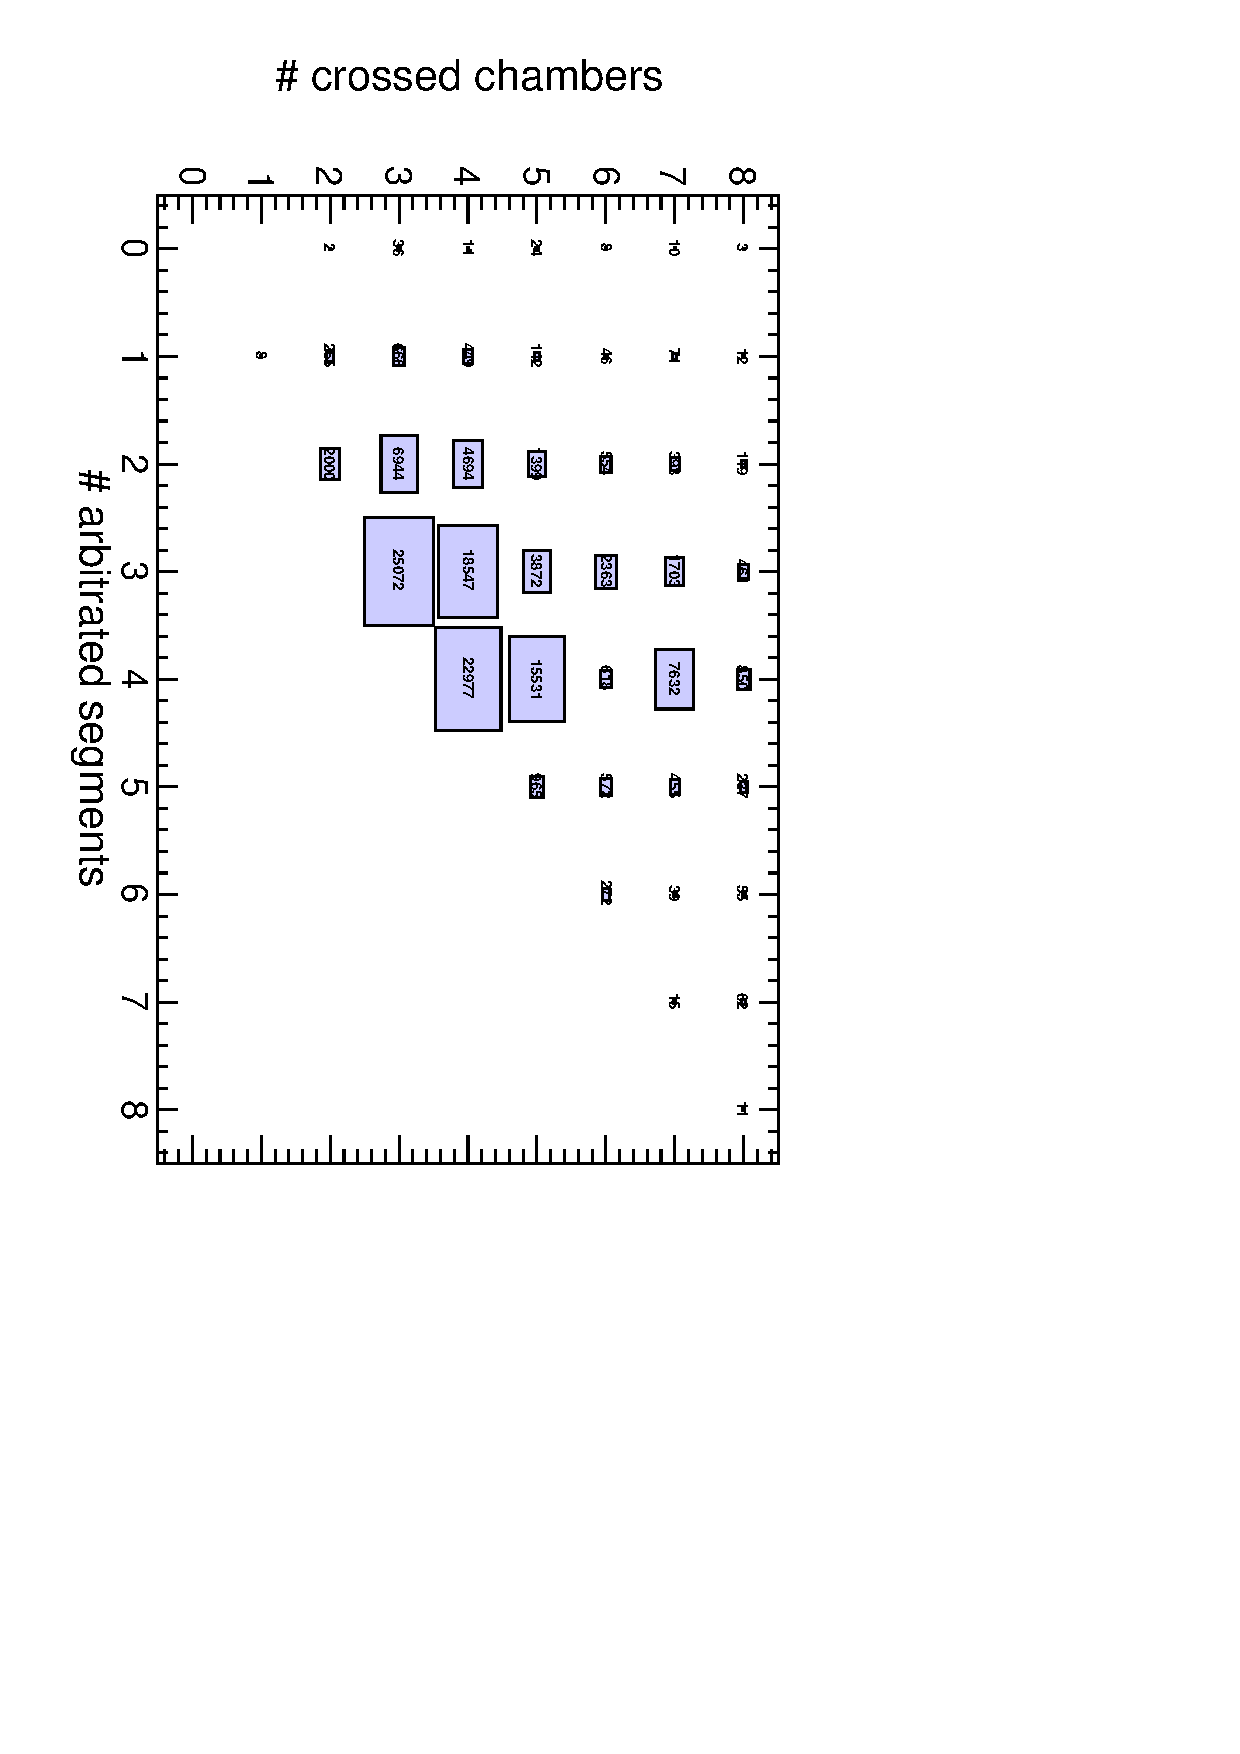
\includegraphics[height=0.85\linewidth, angle=90]{tracks_segments_chambers.pdf}
\end{center}

\vspace{-3 cm}
\hfill (prompt sample) \mbox{\hspace{1.5 cm}}

\vspace{3 cm}
\end{frame}

\begin{frame}
\frametitle{Semi-final set of cuts}

\begin{itemize}
\item Event:
\begin{itemize}
\item HLT\_Mu9 (lowest threshold that is not currently prescaled)
\item one muon with $p_T > 11$~GeV/$c$
\item minimum number of muons for desired number of muon-groups
  (e.g.\ at least 4 muons for 2 muon-groups)
\end{itemize}

\item Muon (applied {\it before} our analysis):
\begin{itemize}
\item $|\vec{p}| > 2.5$~GeV/$c$ (TrackerMuon identification)
\item $\ge 8$ tracker hits (not strictly; applied by whom? track-finding?)
\end{itemize}

\item Muon (applied {\it by} our analysis):
\begin{itemize}
\item \textcolor{blue}{TrackerMuons (GlobalMuons offer no known advantages)}
\item $p_T > 5$~GeV/$c$, $|\eta| < 2.4$ (tighter than defaults)
\item $N_\s{segments} \ge 2$ with track-and-segment arbitration, $|\Delta x| < 3$~cm, $|\Delta x| < 4 \sigma_{\Delta x}$, $|\Delta y| < 5$~cm, $|\Delta y| < 5 \sigma_{\Delta y}$
\end{itemize}

\item \textcolor{blue}{Additional quality cuts}
\begin{itemize}
\item \textcolor{blue}{at least one primary vertex with $|z| < 24$~cm (hn-cms-PO7TeV)}
\item \textcolor{blue}{filter out scraping (Collisions2010Recipes)}
\item \textcolor{blue}{\ldots}
\end{itemize}
\end{itemize}
\end{frame}

\begin{frame}
\frametitle{New: data/MC comparision}
\begin{itemize}
\item Even the best BSM theories predict $\sim$1~pb: we can safely study backgrounds with the existing sample
\begin{itemize}
\item can expect Pythia normalizations to be wrong by a factor of a
  few (and differently for resonances as for b-jets)
\item but we want to understand and protect ourselves against
  differences in distributions
\end{itemize}

\item Select runs/lumisections with good tracker, muon (including RPC), and trigger; ignore quality of calorimeters (gain a factor of 1.5)
\item Consider only {\tt /Mu/Run2010A-PromptReco-{\bf v4}/RECO}
  (137437--142467, or Jun~10--Aug~07) when primary datasets were already set up; modern triggers; most of the good data
\item Integrated luminosity:
\begin{itemize}
\item HLT\_Mu5 (prescaled starting 141956, requires L1SingleMu3): 333.75~nb$^{-1}$
\item HLT\_Mu9 (unprescaled, requires L1SingleMu7): 592.78~nb$^{-1}$
\end{itemize}
\item Following all recommended recipes (RunRegistry, lumicalc.py, etc.)
\end{itemize}
\end{frame}

\begin{frame}
\frametitle{Resolved initial troubles}
\begin{itemize}
\item I apparently don't know the proper way to apply trigger cuts using offline variables
\begin{itemize}
\item on my first attempt, factor-of-10 discrepancy between normalizations of data and MC
\item tracked down to the way I was selecting ``HLT\_Mu9 passed'' events
\item when I apply the same requirement in a different way, we get near-perfect agreement
\item I have external reasons for being more confident in method~\#2,
because it's copied from the way it was done in AlCaReco production
(set up by experts)
\item method~\#2 is less convenient because it requires whole samples
to be cut, not an ntuple-level thing
\end{itemize}

\item Because of this, the following pages will have data selected by
HLT\_Mu9, MC with no trigger requirement, and both with $pT_1 >
11$~GeV/$c$ ($pT_1$ is the leading-muon $p_T$)
\end{itemize}
\end{frame}

\begin{frame}
\frametitle{Mass distribution}
\begin{itemize}
\item Out-of-the-box, normalization of everything except the
resonances seems to be pretty good after all
\item Reminder of cuts: opposite-sign, $p_T > 5$~GeV/$c$ TrackerMuons with $N_\s{segments} \ge 2$ (arbitrated), HLT\_Mu9 in data only, $pT_1 > 11$~GeV/$c$
\end{itemize}

\vfill
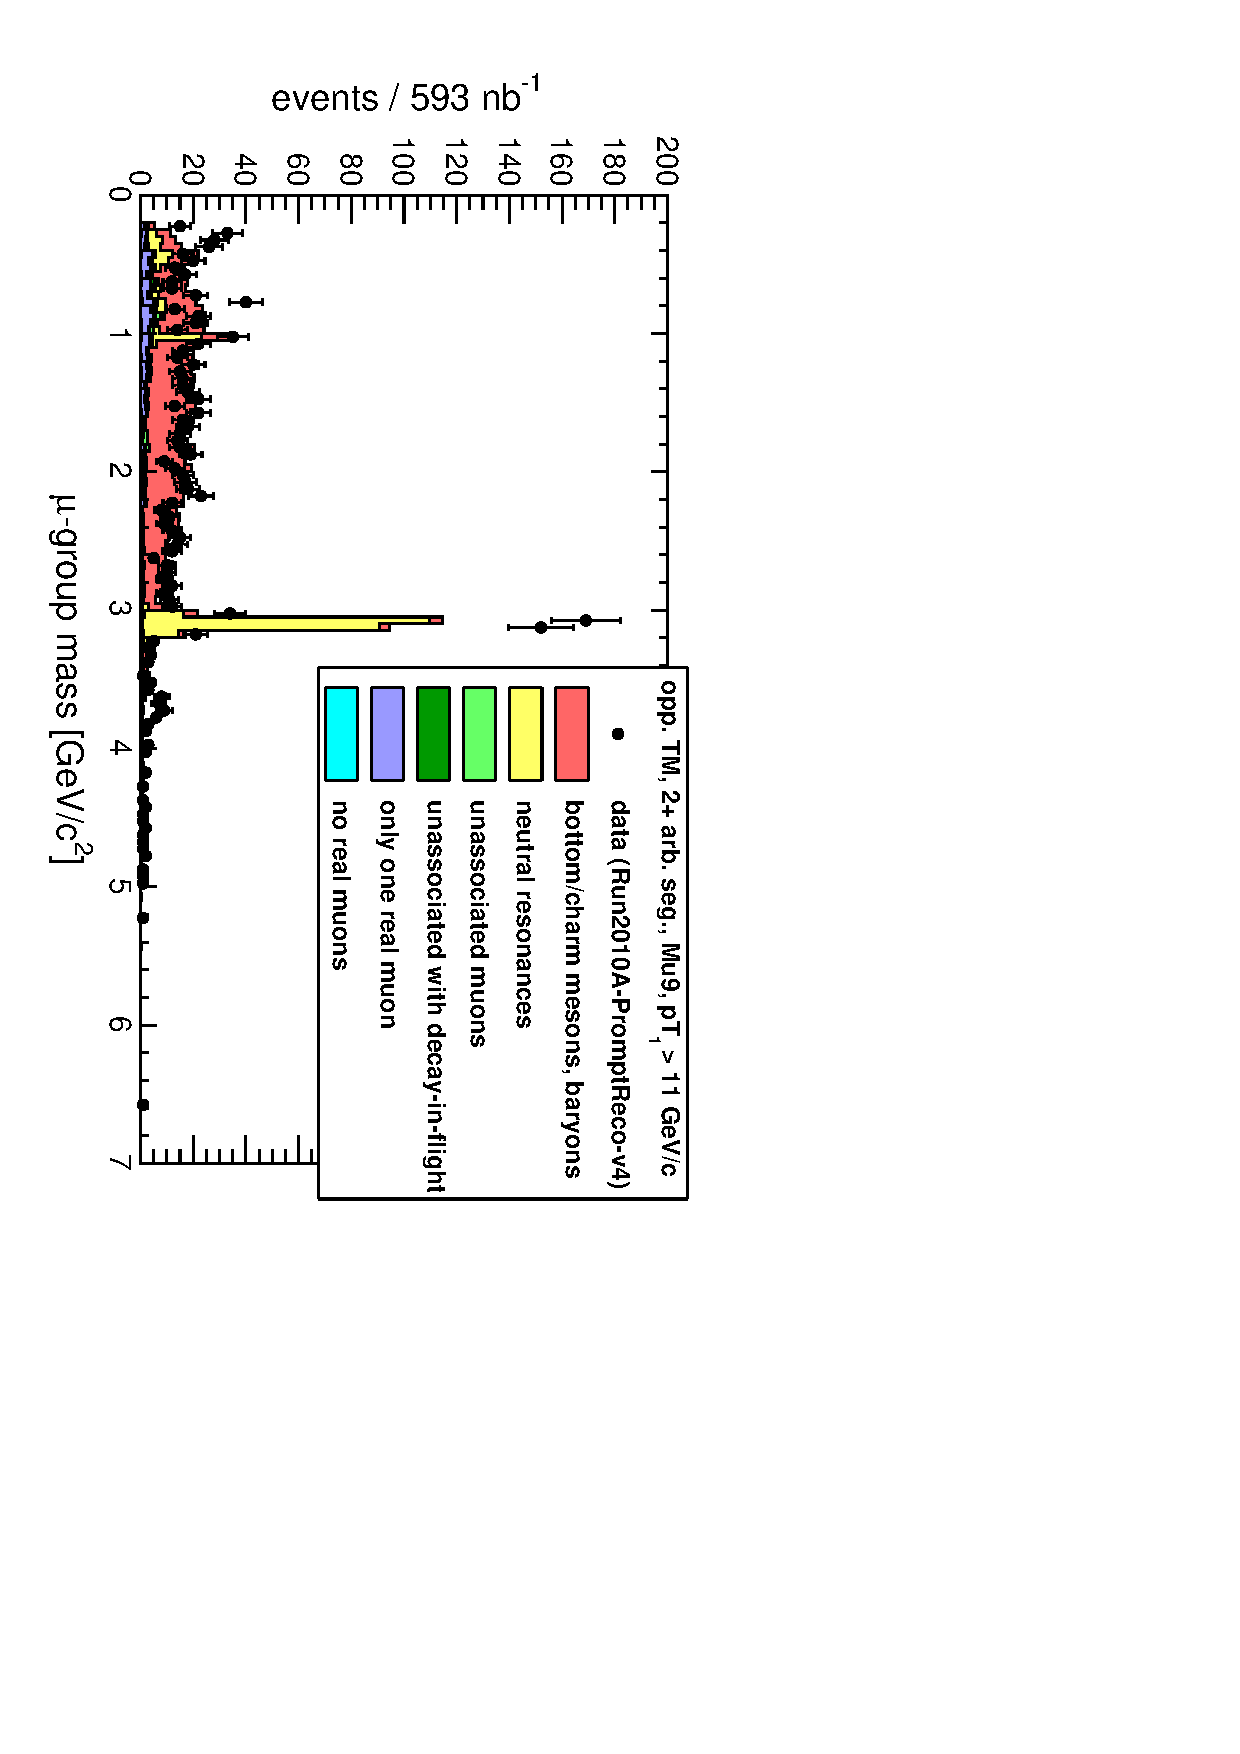
\includegraphics[height=\linewidth, angle=90]{Mu9_mass_general.pdf}
\end{frame}

\begin{frame}
\frametitle{Mass distribution}
\begin{itemize}
\item Attempt to correct MC by (inappropriately) scaling the resonances
\begin{itemize}
\item $J/\psi$ increased by 1.48
\item $\eta(548)$ increased by 5.2
\item $\omega(782)$ and $\psi(2S)$ are {\it missing} from MC
\item $\phi(1020)$ looks right \mbox{(but wasn't $s$, $\bar{s}$ overproduced in our MC?)\hspace{-1 cm}}
\end{itemize}
\end{itemize}

\vfill
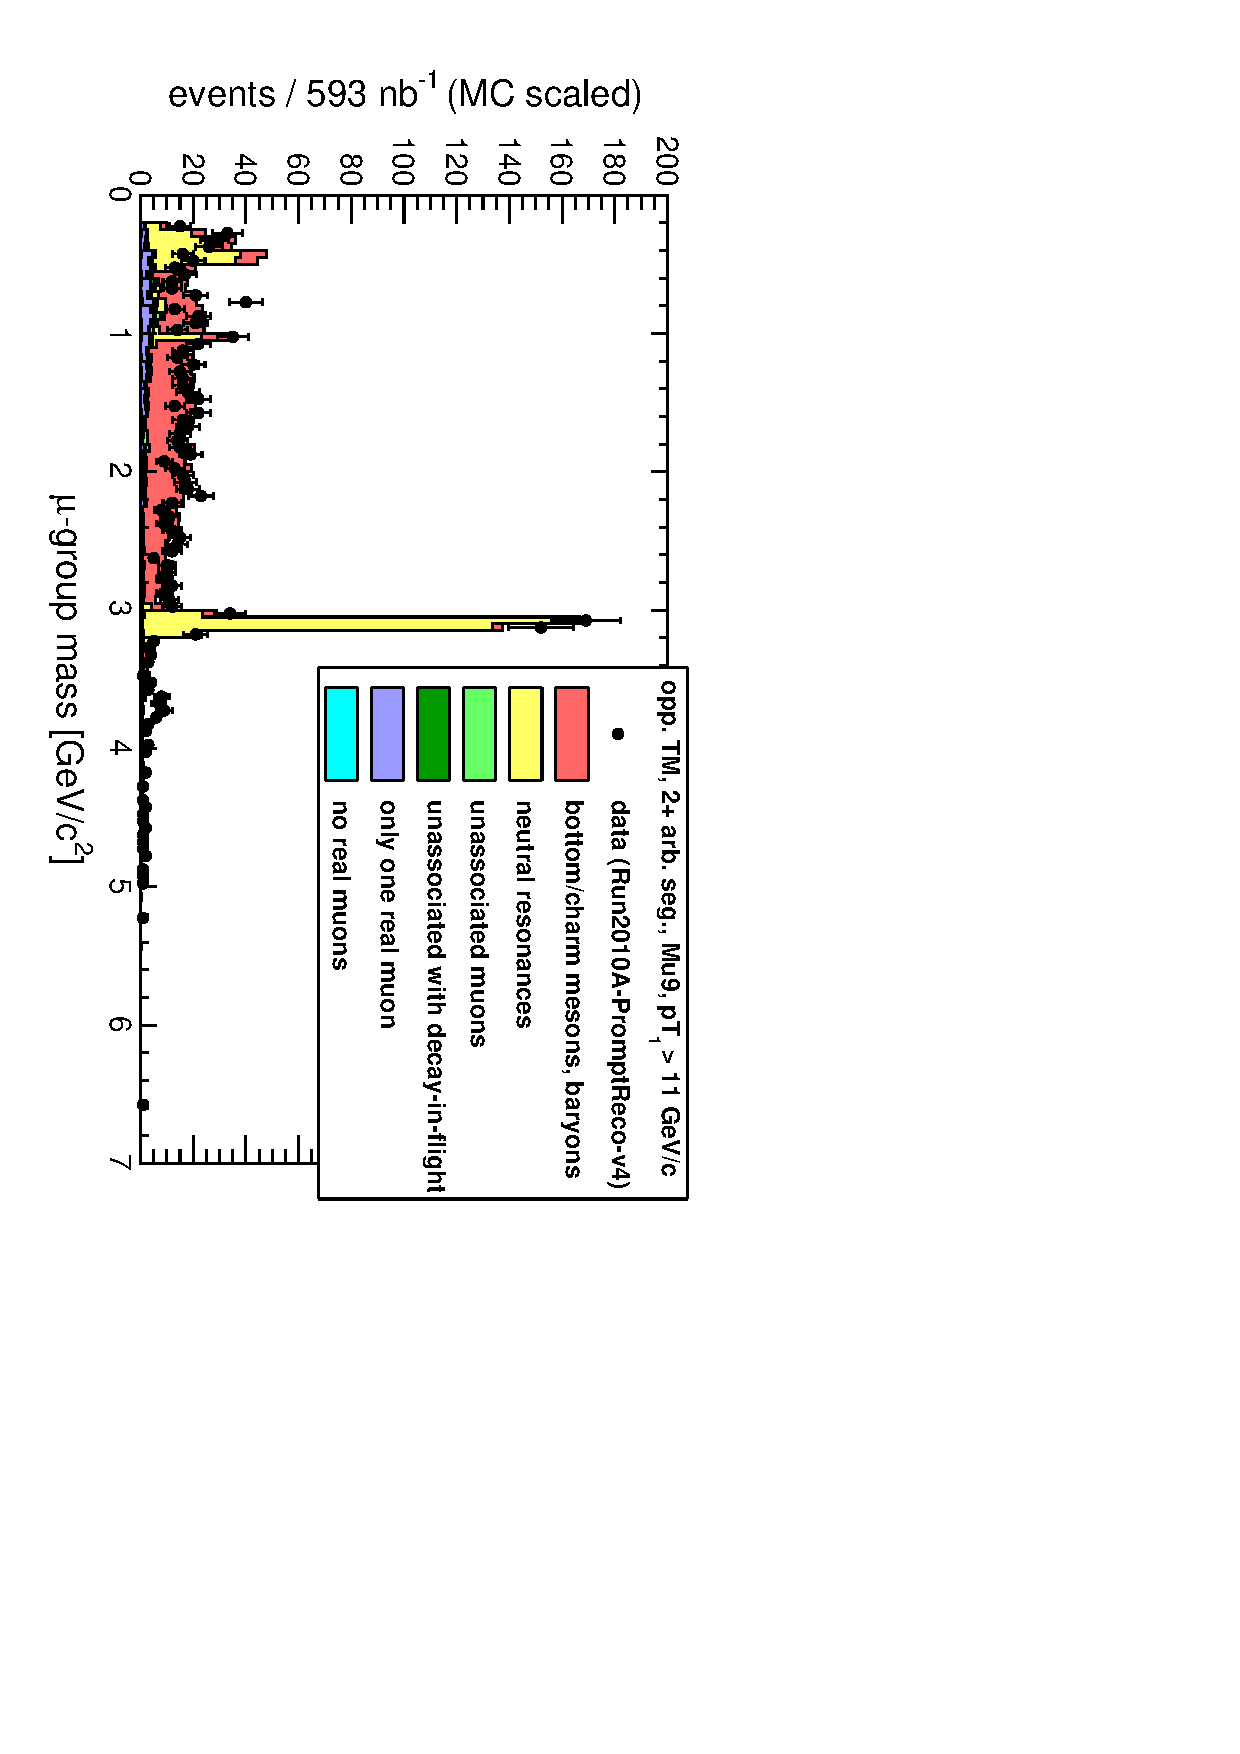
\includegraphics[height=\linewidth, angle=90]{Mu9_mass_scaled.pdf}
\end{frame}

\begin{frame}
\frametitle{$p_T$ spectrum \only<1>{{\it without} scaling}\only<2>{{\it with} scaling}}
\begin{itemize}
\item This is $p_T$ of the muon-groups (can only be less than
16~GeV/$c$ if the muon group does not contain the leading muon; can
never be below 10~GeV/$c$)
\item Scaling does not reproduce the shape of the distribution
\end{itemize}

\vfill
\only<1>{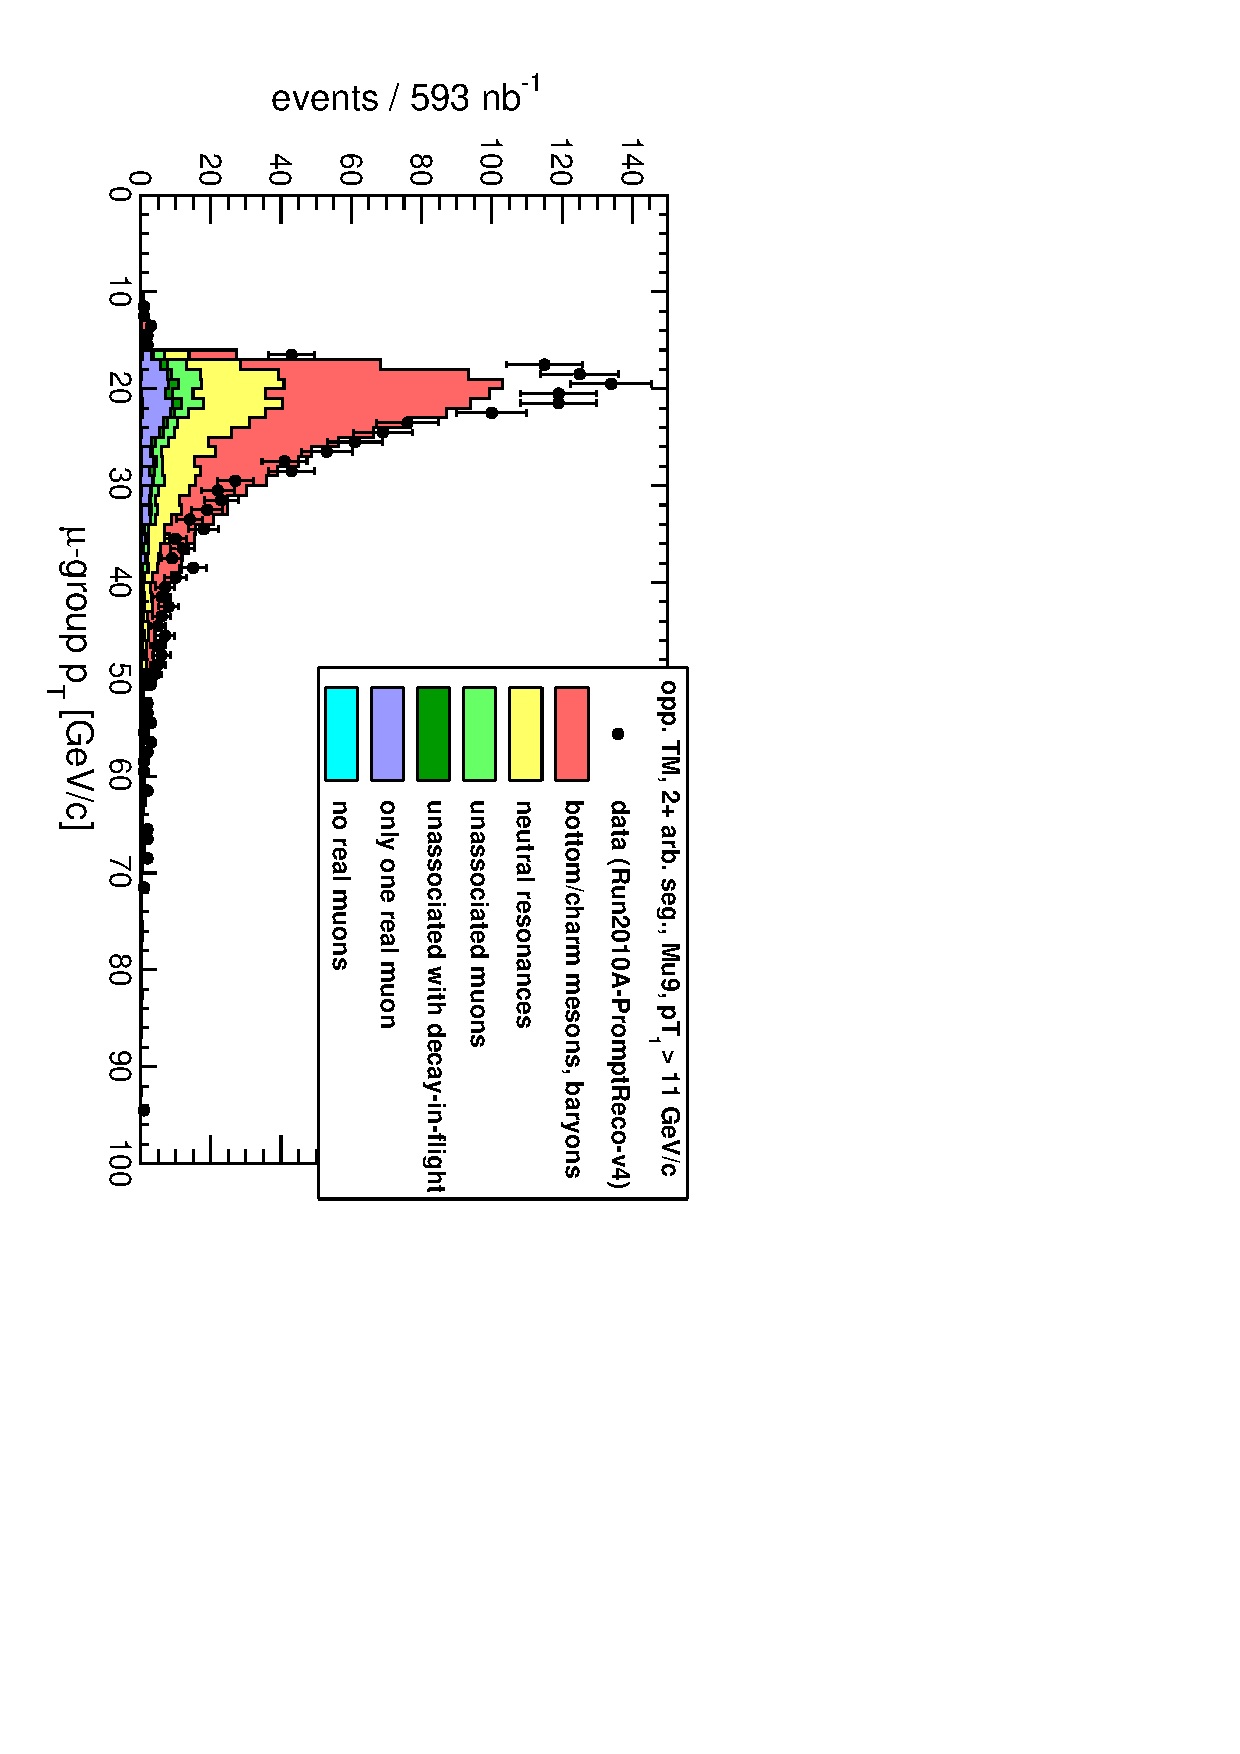
\includegraphics[height=\linewidth, angle=90]{Mu9_pt.pdf}}
\only<2>{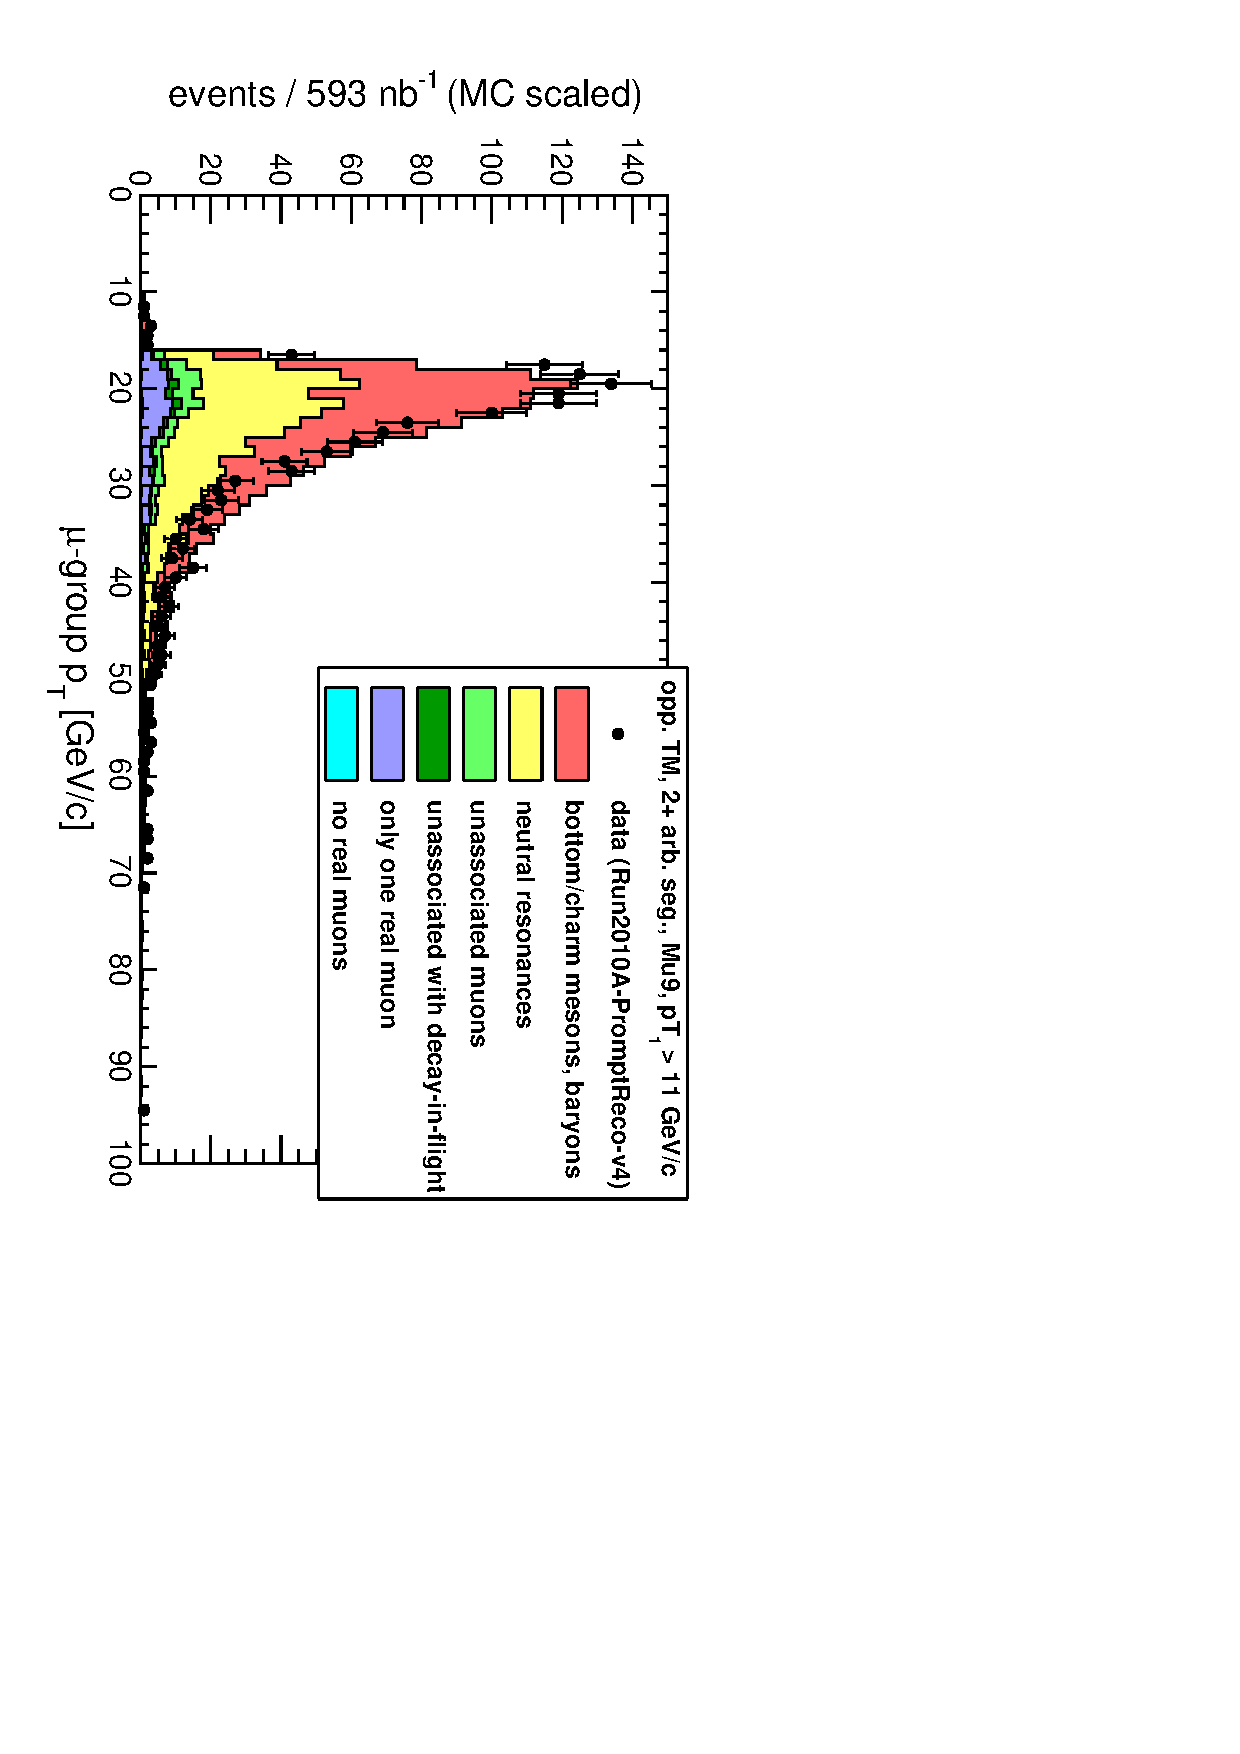
\includegraphics[height=\linewidth, angle=90]{Mu9_pt_scaled.pdf}}
\end{frame}

\begin{frame}
\frametitle{$p_T$ spectrum}
\begin{itemize}
\item In more detail: look at only $J/\psi$ mass region
\item Clearly, it's just because we're missing the prompt $J/\psi$
(and $\psi(2S)$) contributions {\scriptsize (if I include those MC
samples, then perhaps everything will line up without any
MC-tuning\ldots)}
\end{itemize}

\vfill
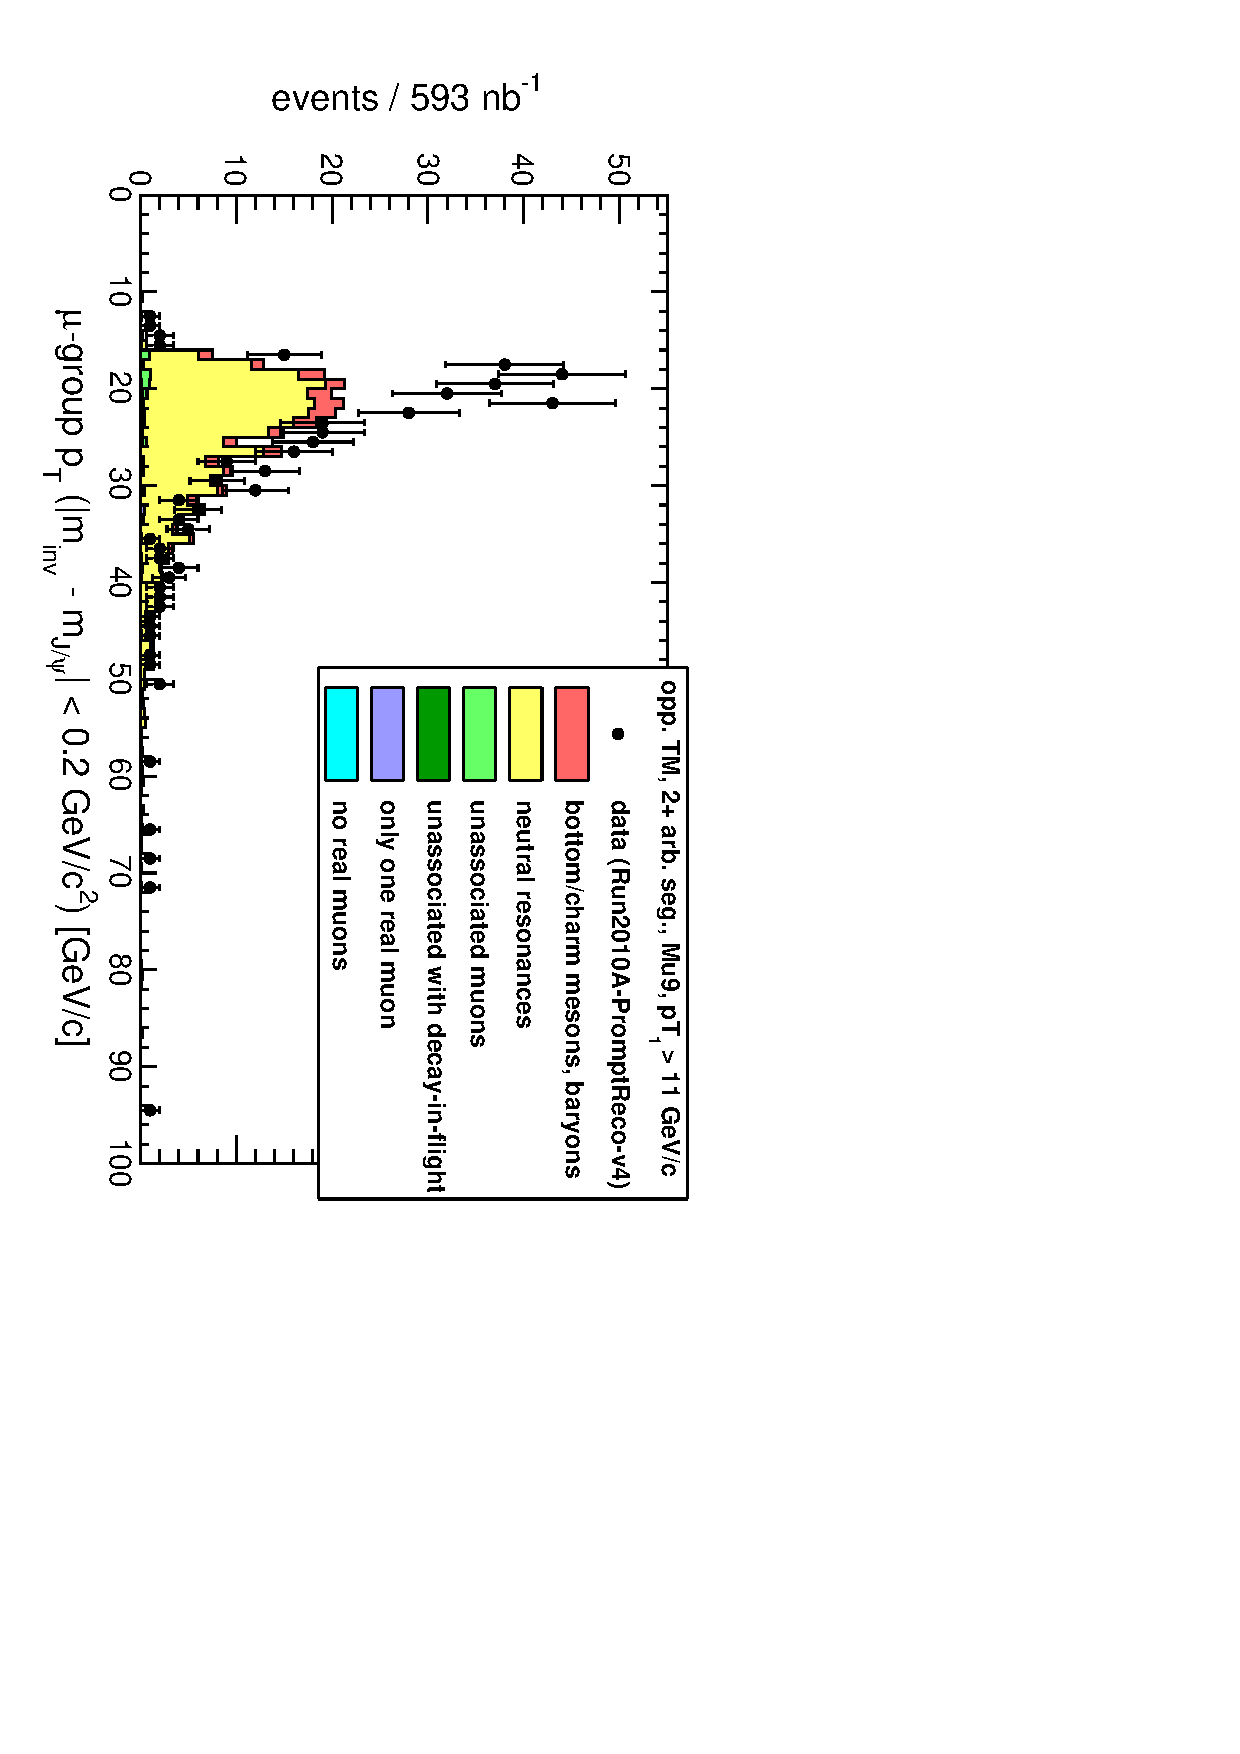
\includegraphics[height=\linewidth, angle=90]{Mu9_pt_jpsi.pdf}
\end{frame}

\begin{frame}
\frametitle{Gallery of resonances}

\begin{columns}
\column{0.4\linewidth}
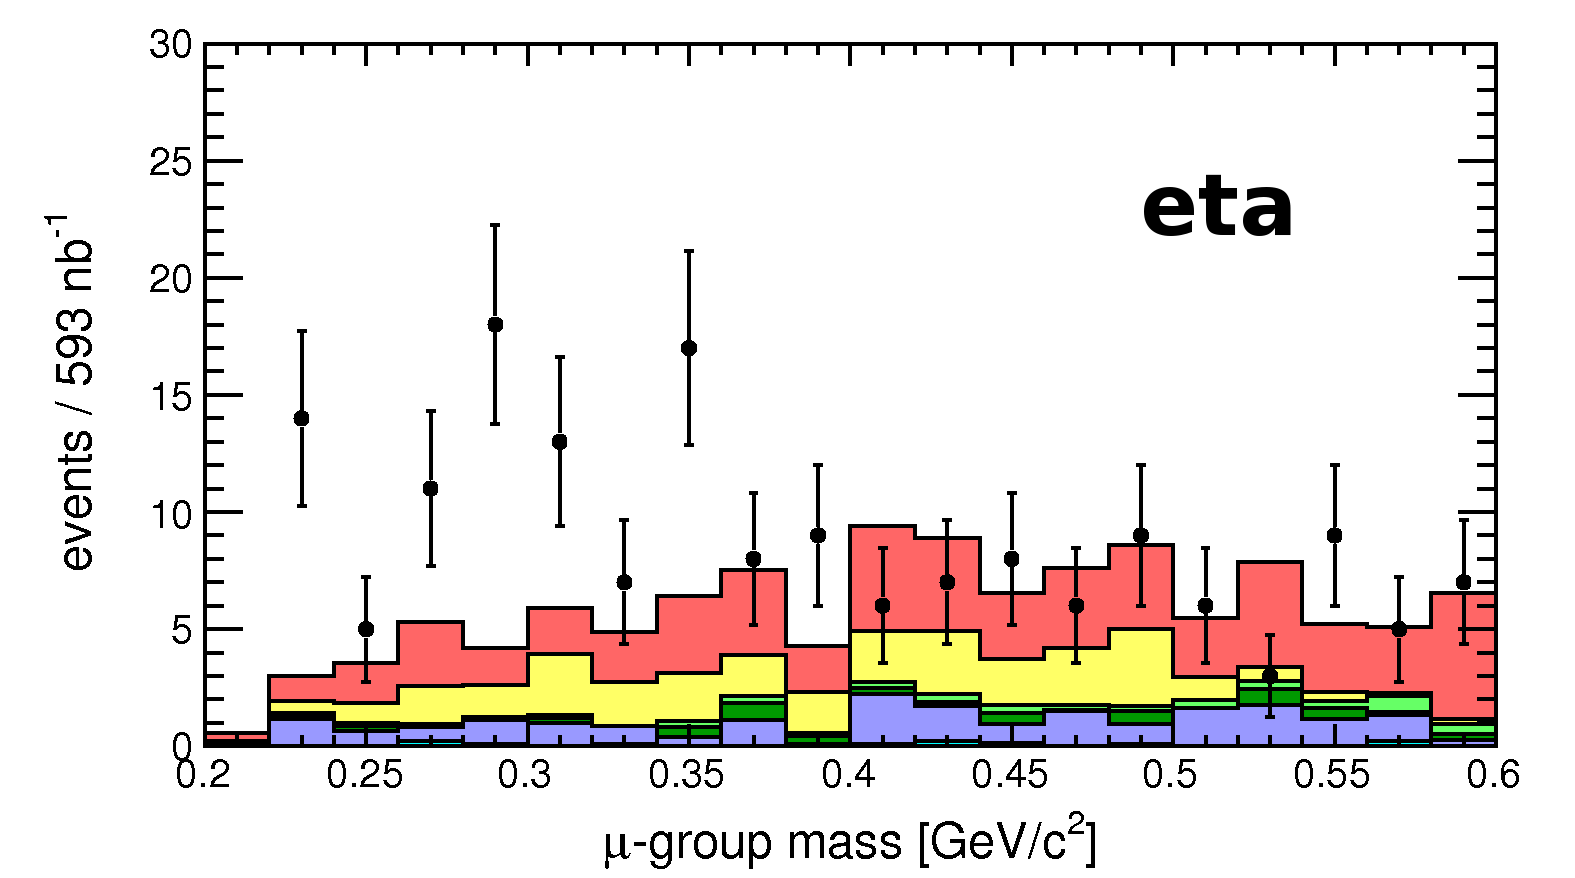
\includegraphics[width=\linewidth]{Mu9_mass_eta.png}

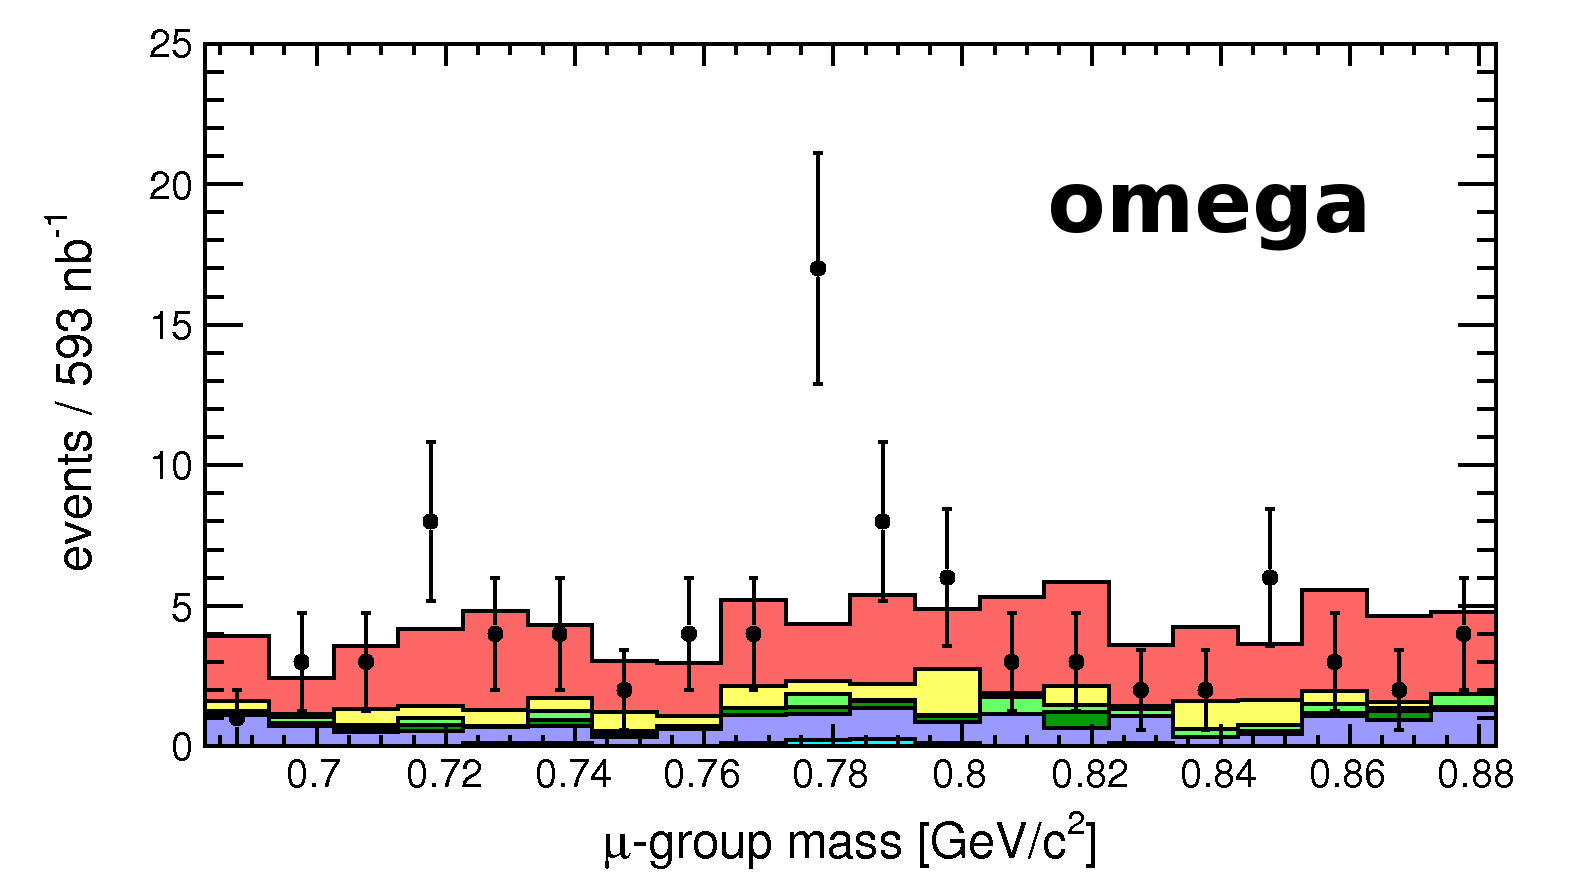
\includegraphics[width=\linewidth]{Mu9_mass_omg.png}

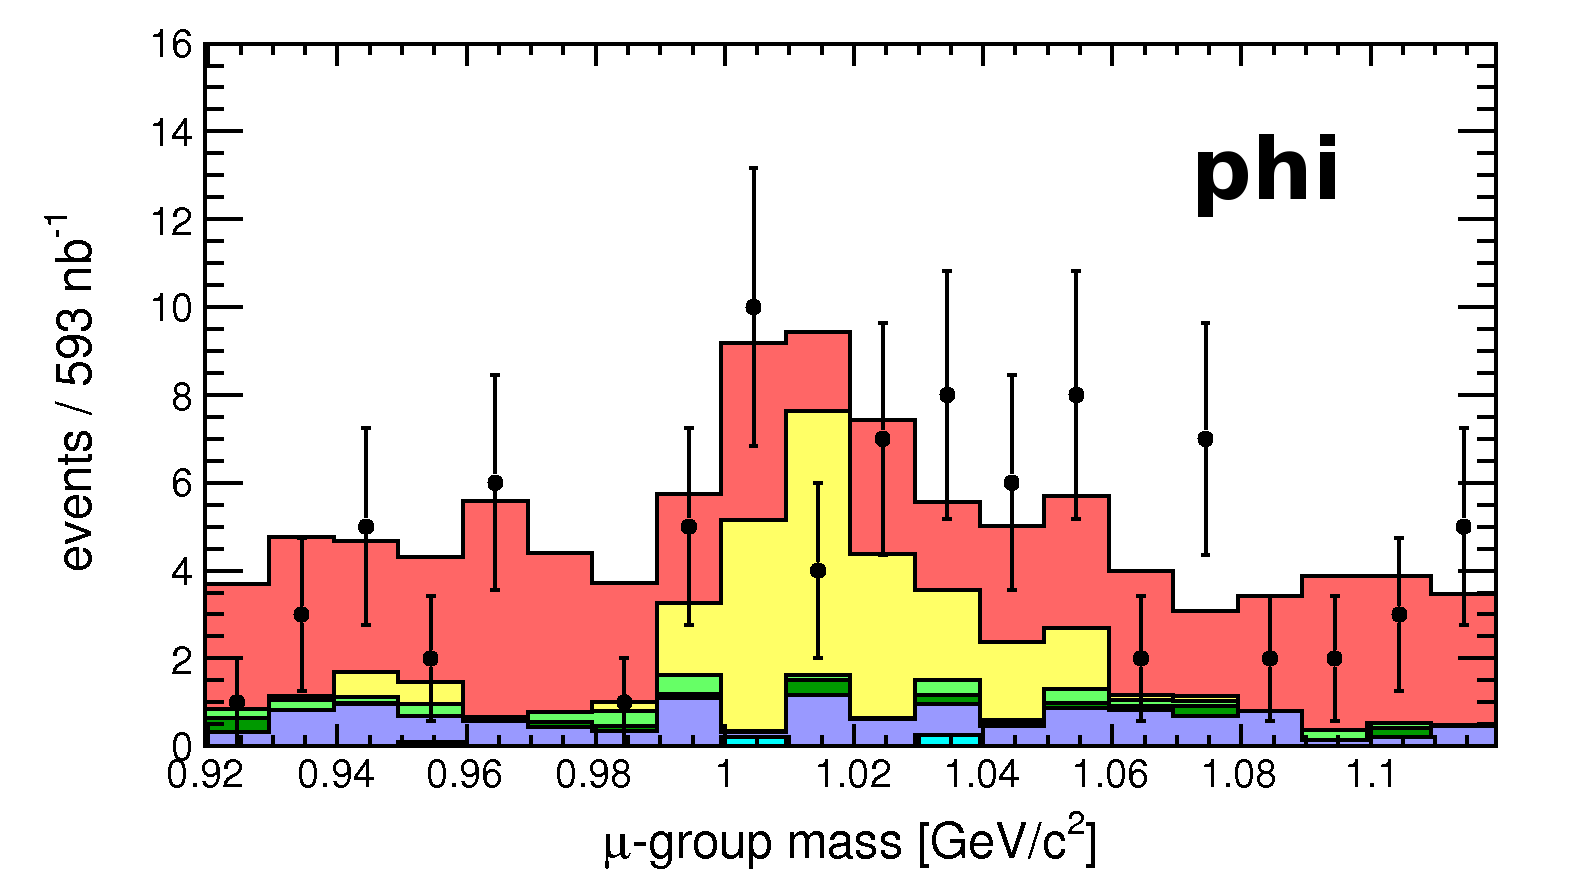
\includegraphics[width=\linewidth]{Mu9_mass_phi.png}

\column{0.6\linewidth}
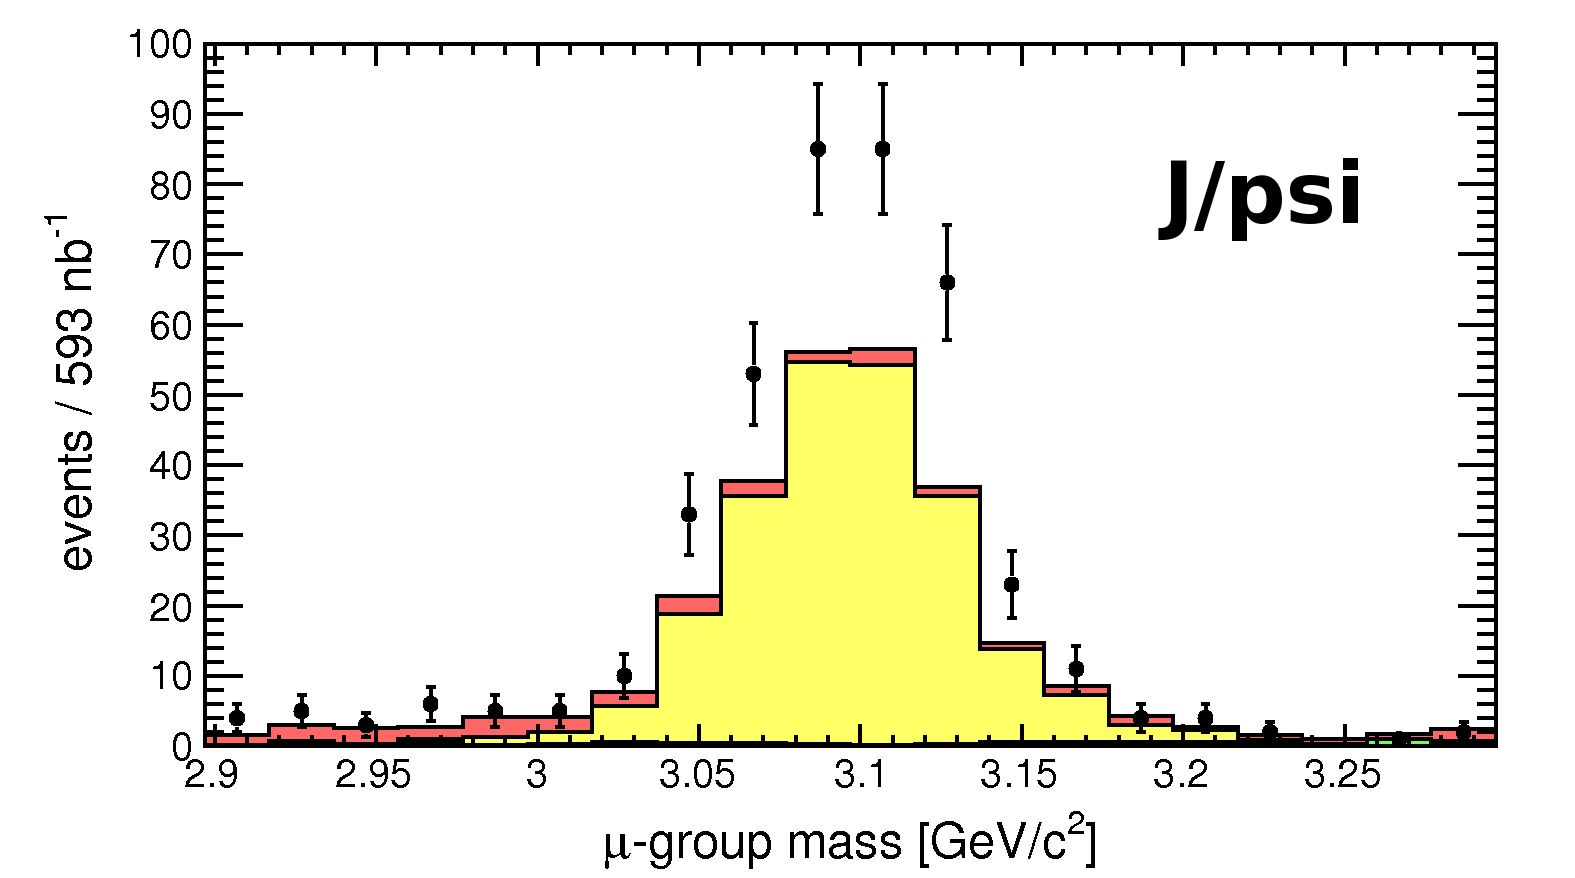
\includegraphics[width=\linewidth]{Mu9_mass_jpsi.png}

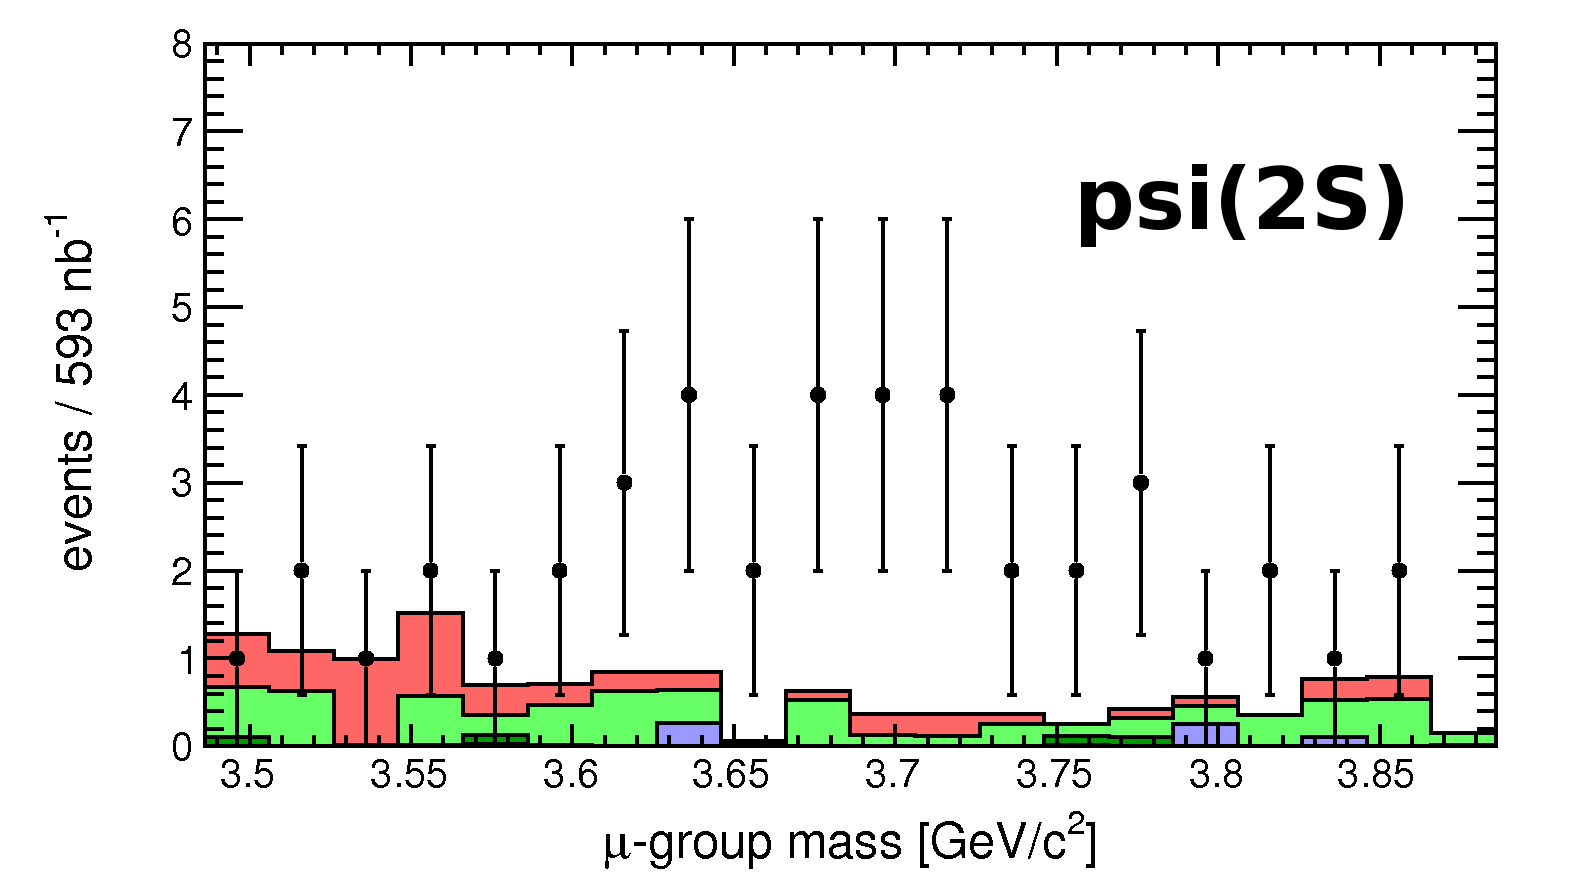
\includegraphics[width=\linewidth]{Mu9_mass_psi2s.png}

\end{columns}
\end{frame}

\begin{frame}
\frametitle{Low-mass stuff isn't right}

\begin{columns}
\column{0.7\linewidth}
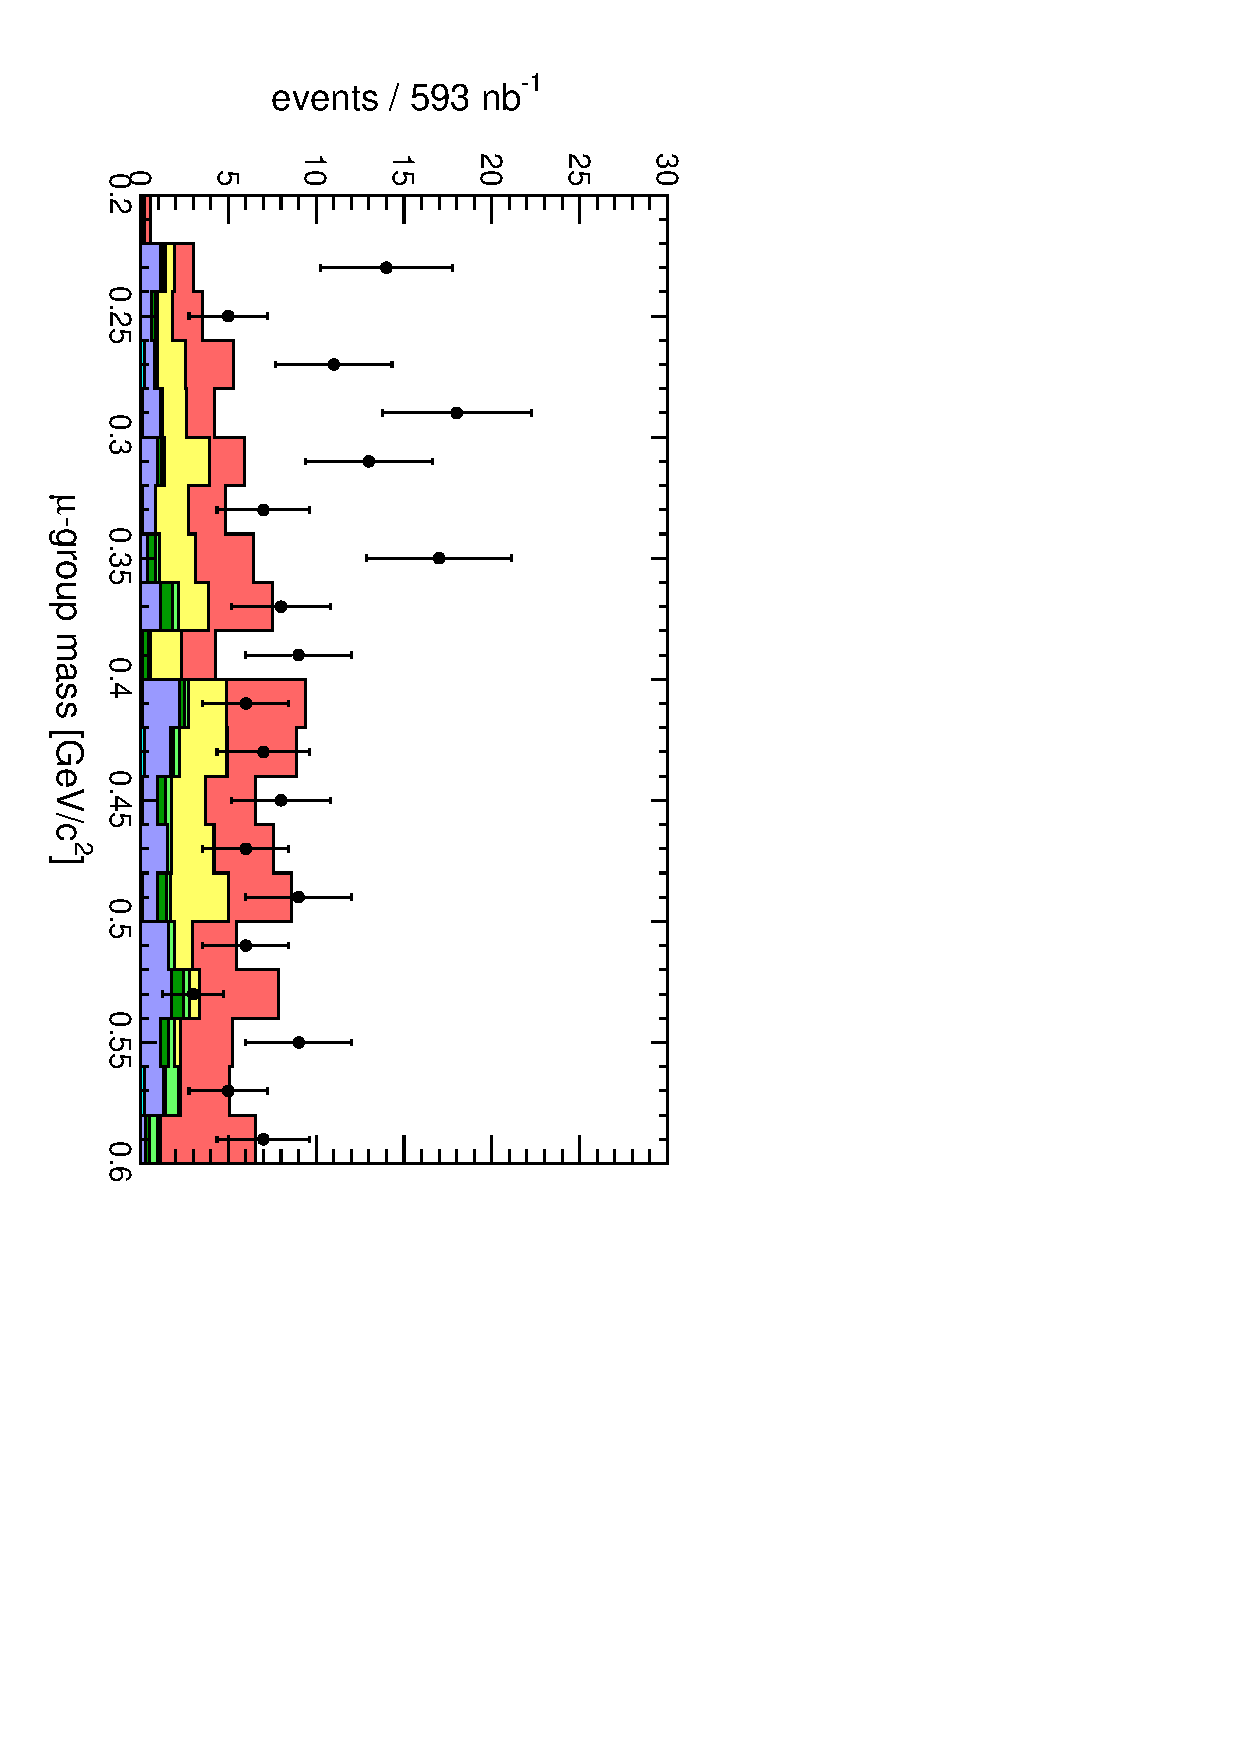
\includegraphics[height=\linewidth, angle=90]{Mu9_mass_eta.pdf}

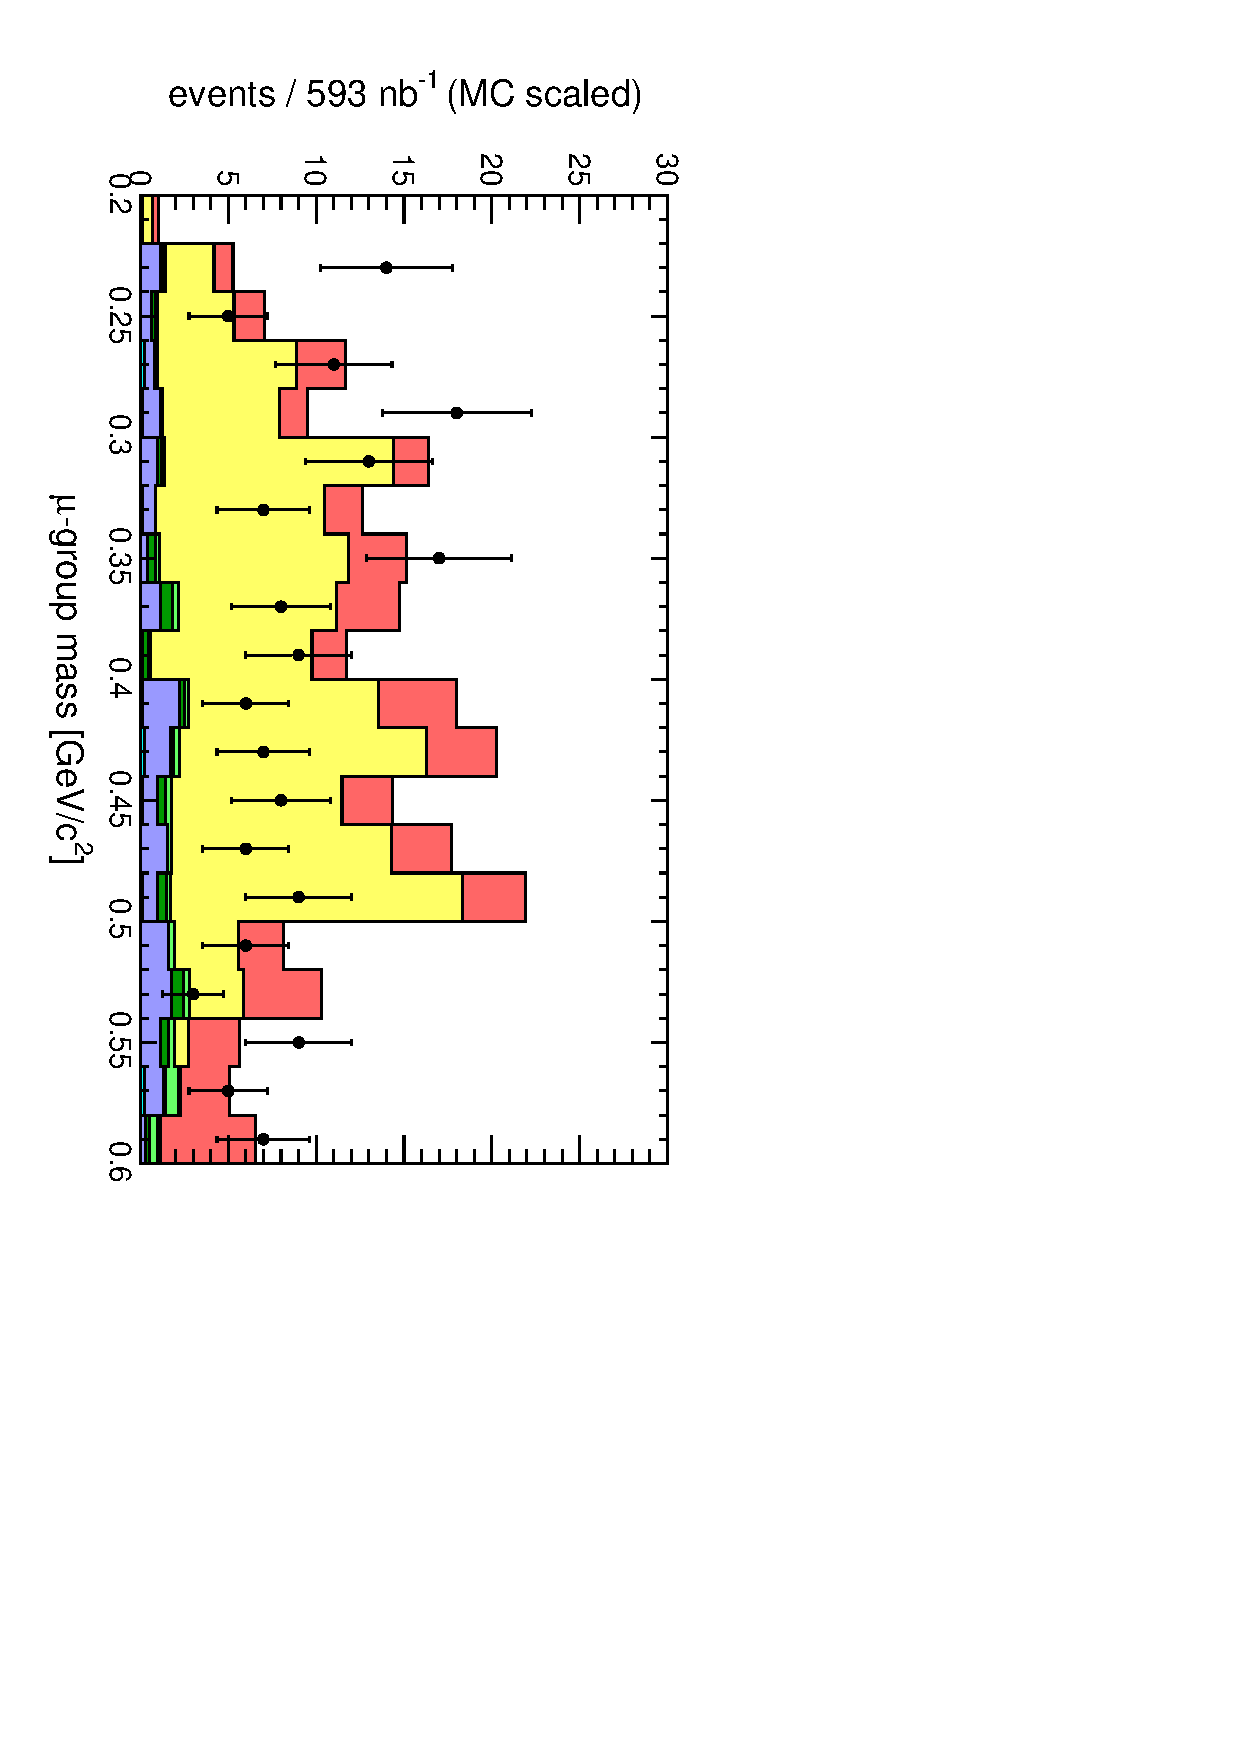
\includegraphics[height=\linewidth, angle=90]{Mu9_mass_eta_scaled.pdf}

\column{0.3\linewidth}
Scaling the $\eta$s by 5.2 is a completely wrong thing to do
\end{columns}
\end{frame}

\begin{frame}
\frametitle{Remaining slides} Everything from this point onward is
repeated for the Mu5 trigger/7~GeV/$c$ cut, where we get to see some
of the resonances more clearly because they are produced with lower
momenta

\vspace{1 cm}
(This is where I ran out of time, writing this talk)
\end{frame}

\begin{frame}
\frametitle{Mass distribution}
\begin{itemize}
\item Out-of-the-box, normalization of everything except the
resonances seems to be pretty good after all
\item Reminder of cuts: opposite-sign, $p_T > 5$~GeV/$c$ TrackerMuons with $N_\s{segments} \ge 2$ (arbitrated), HLT\_Mu5 in data only, $pT_1 > 7$~GeV/$c$
\end{itemize}

\vfill
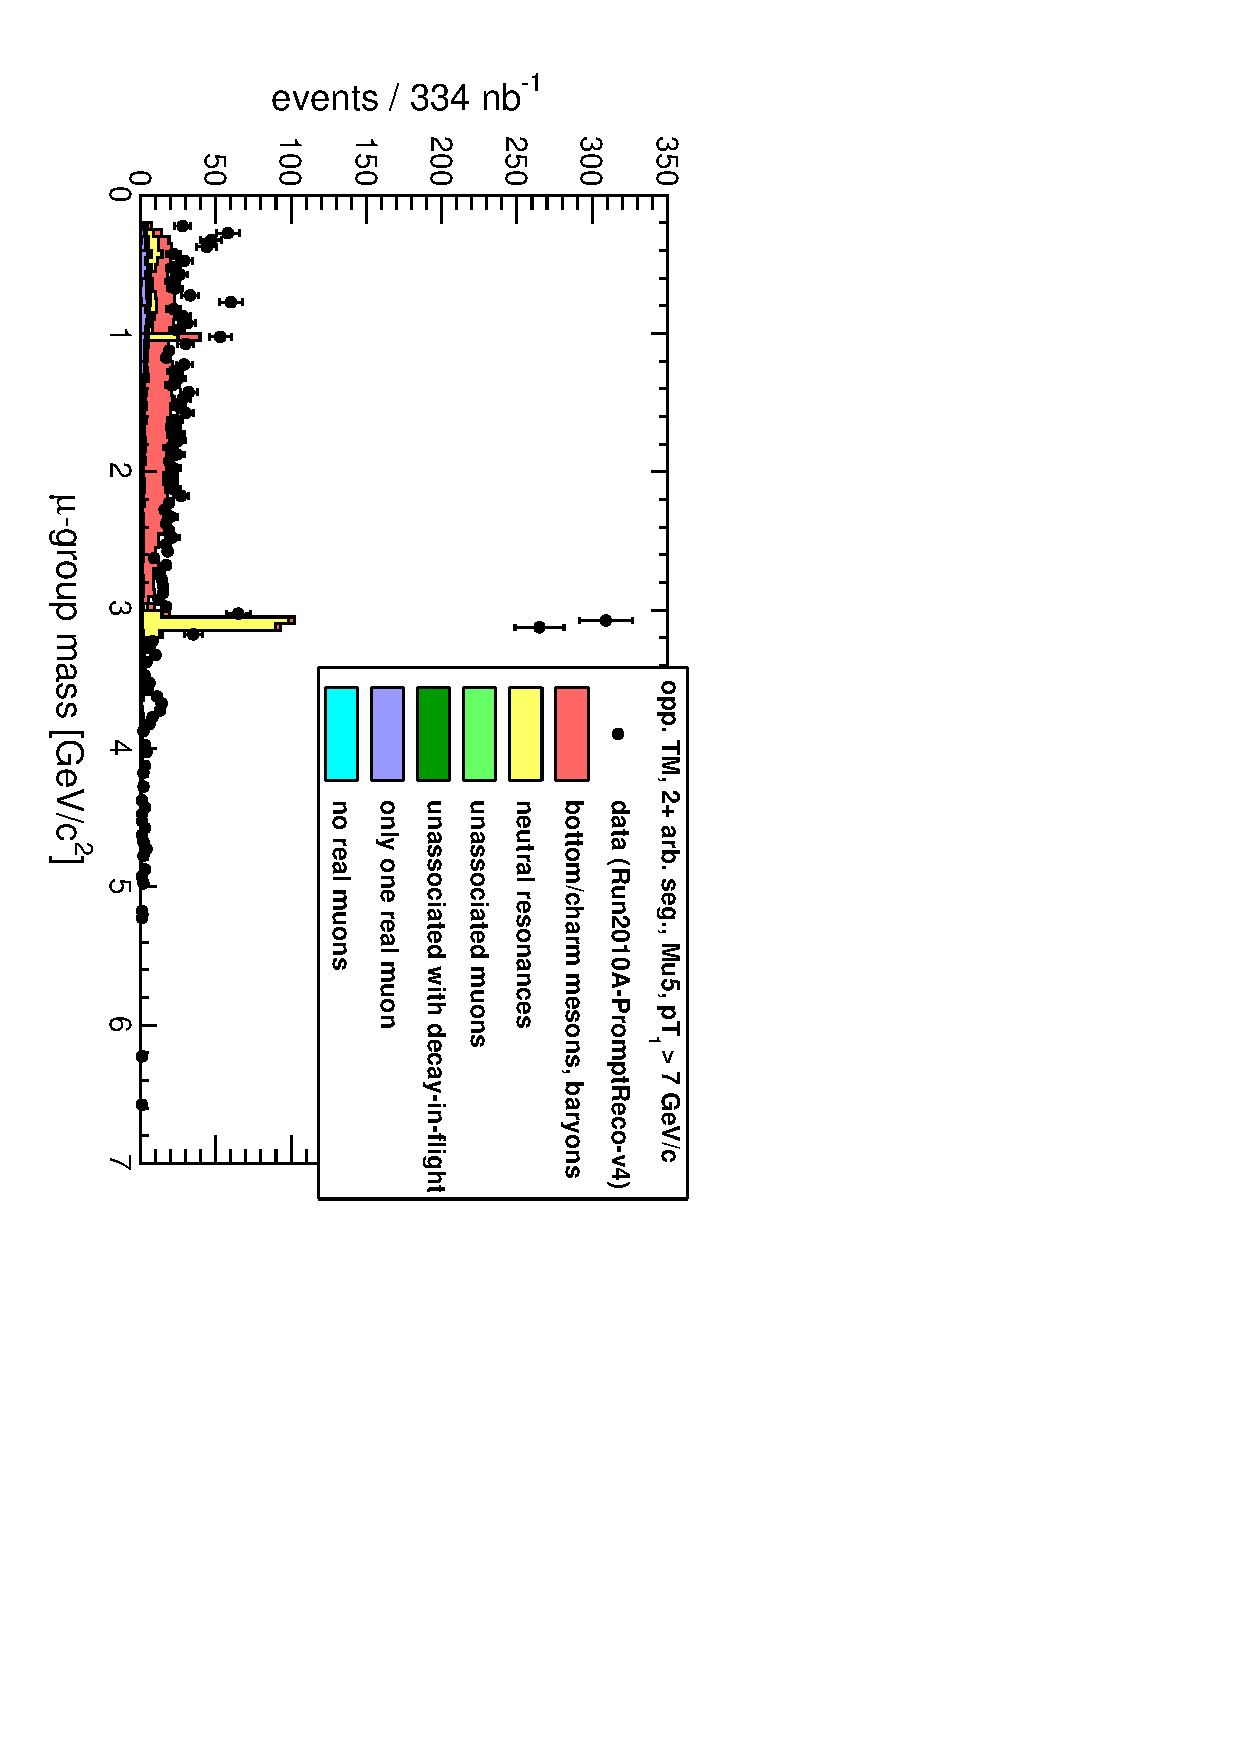
\includegraphics[height=\linewidth, angle=90]{Mu5_mass_general.pdf}
\end{frame}

\begin{frame}
\frametitle{Mass distribution}
\begin{itemize}
\item Attempt to correct MC by (inappropriately) scaling the resonances
\begin{itemize}
\item $J/\psi$ increased by 1.48
\item $\eta(548)$ increased by 5.2
\item $\omega(782)$ and $\psi(2S)$ are {\it missing} from MC
\item $\phi(1020)$ looks right \mbox{(but wasn't $s$, $\bar{s}$ overproduced in our MC?)\hspace{-1 cm}}
\end{itemize}
\end{itemize}

\vfill
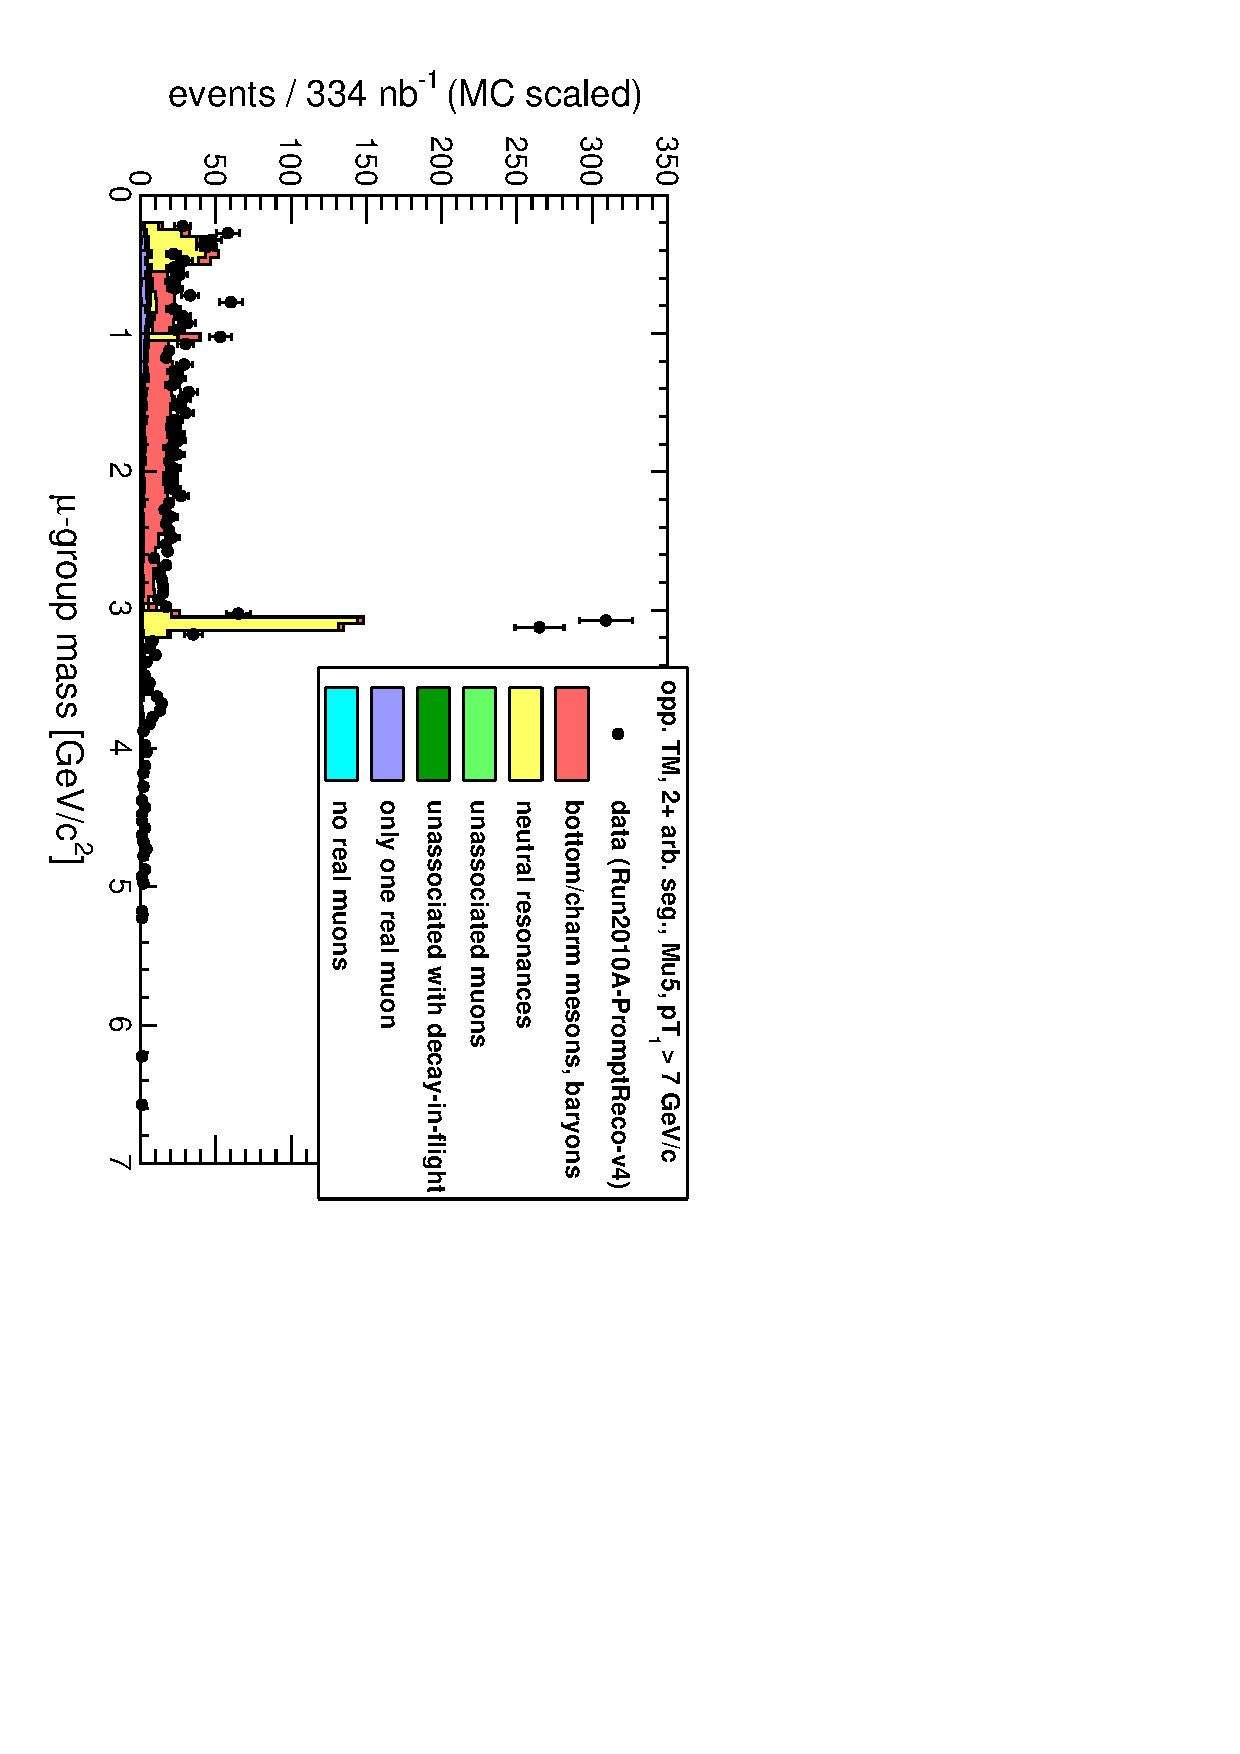
\includegraphics[height=\linewidth, angle=90]{Mu5_mass_scaled.pdf}
\end{frame}

\begin{frame}
\frametitle{$p_T$ spectrum \only<1>{{\it without} scaling}\only<2>{{\it with} scaling}}
\begin{itemize}
\item This is $p_T$ of the muon-groups (can only be less than
16~GeV/$c$ if the muon group does not contain the leading muon; can
never be below 10~GeV/$c$)
\item Scaling does not reproduce the shape of the distribution
\end{itemize}

\vfill
\only<1>{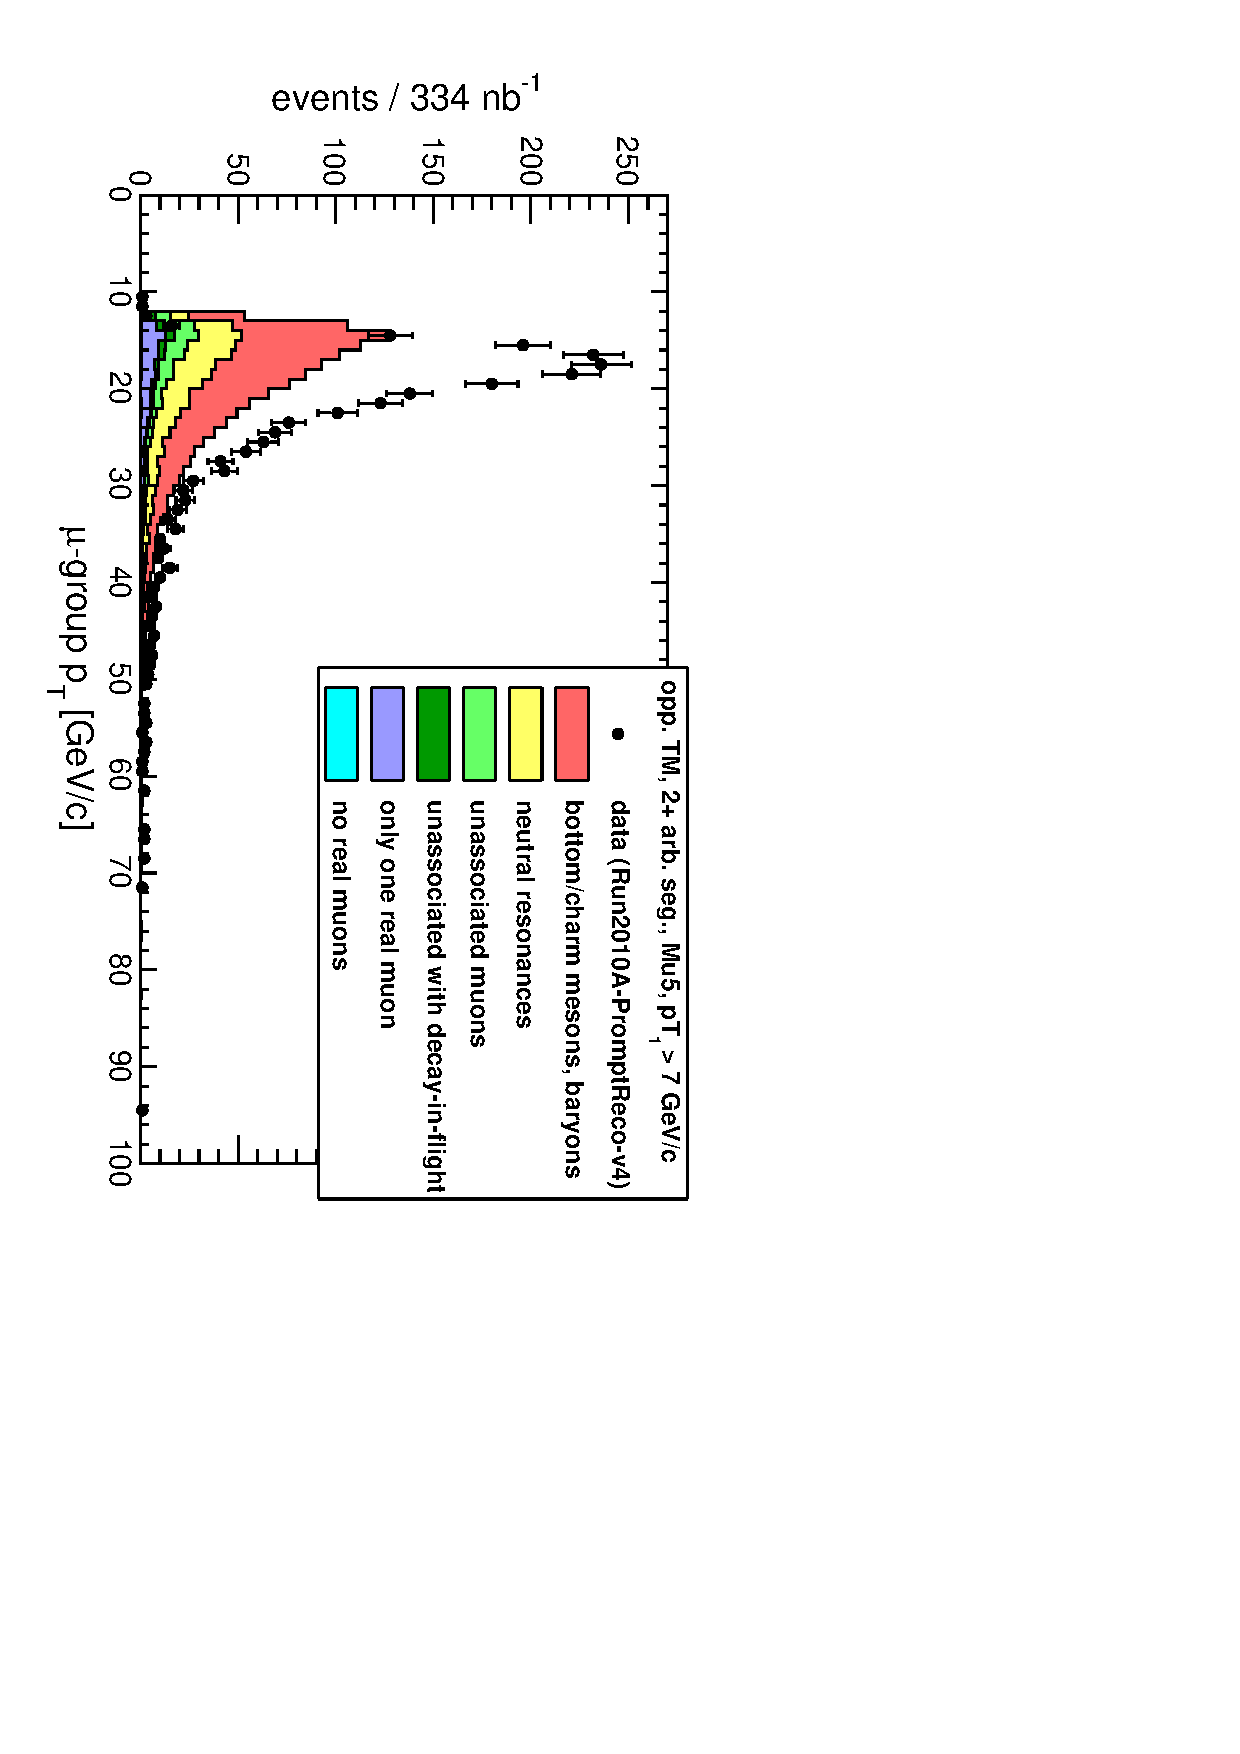
\includegraphics[height=\linewidth, angle=90]{Mu5_pt.pdf}}
\only<2>{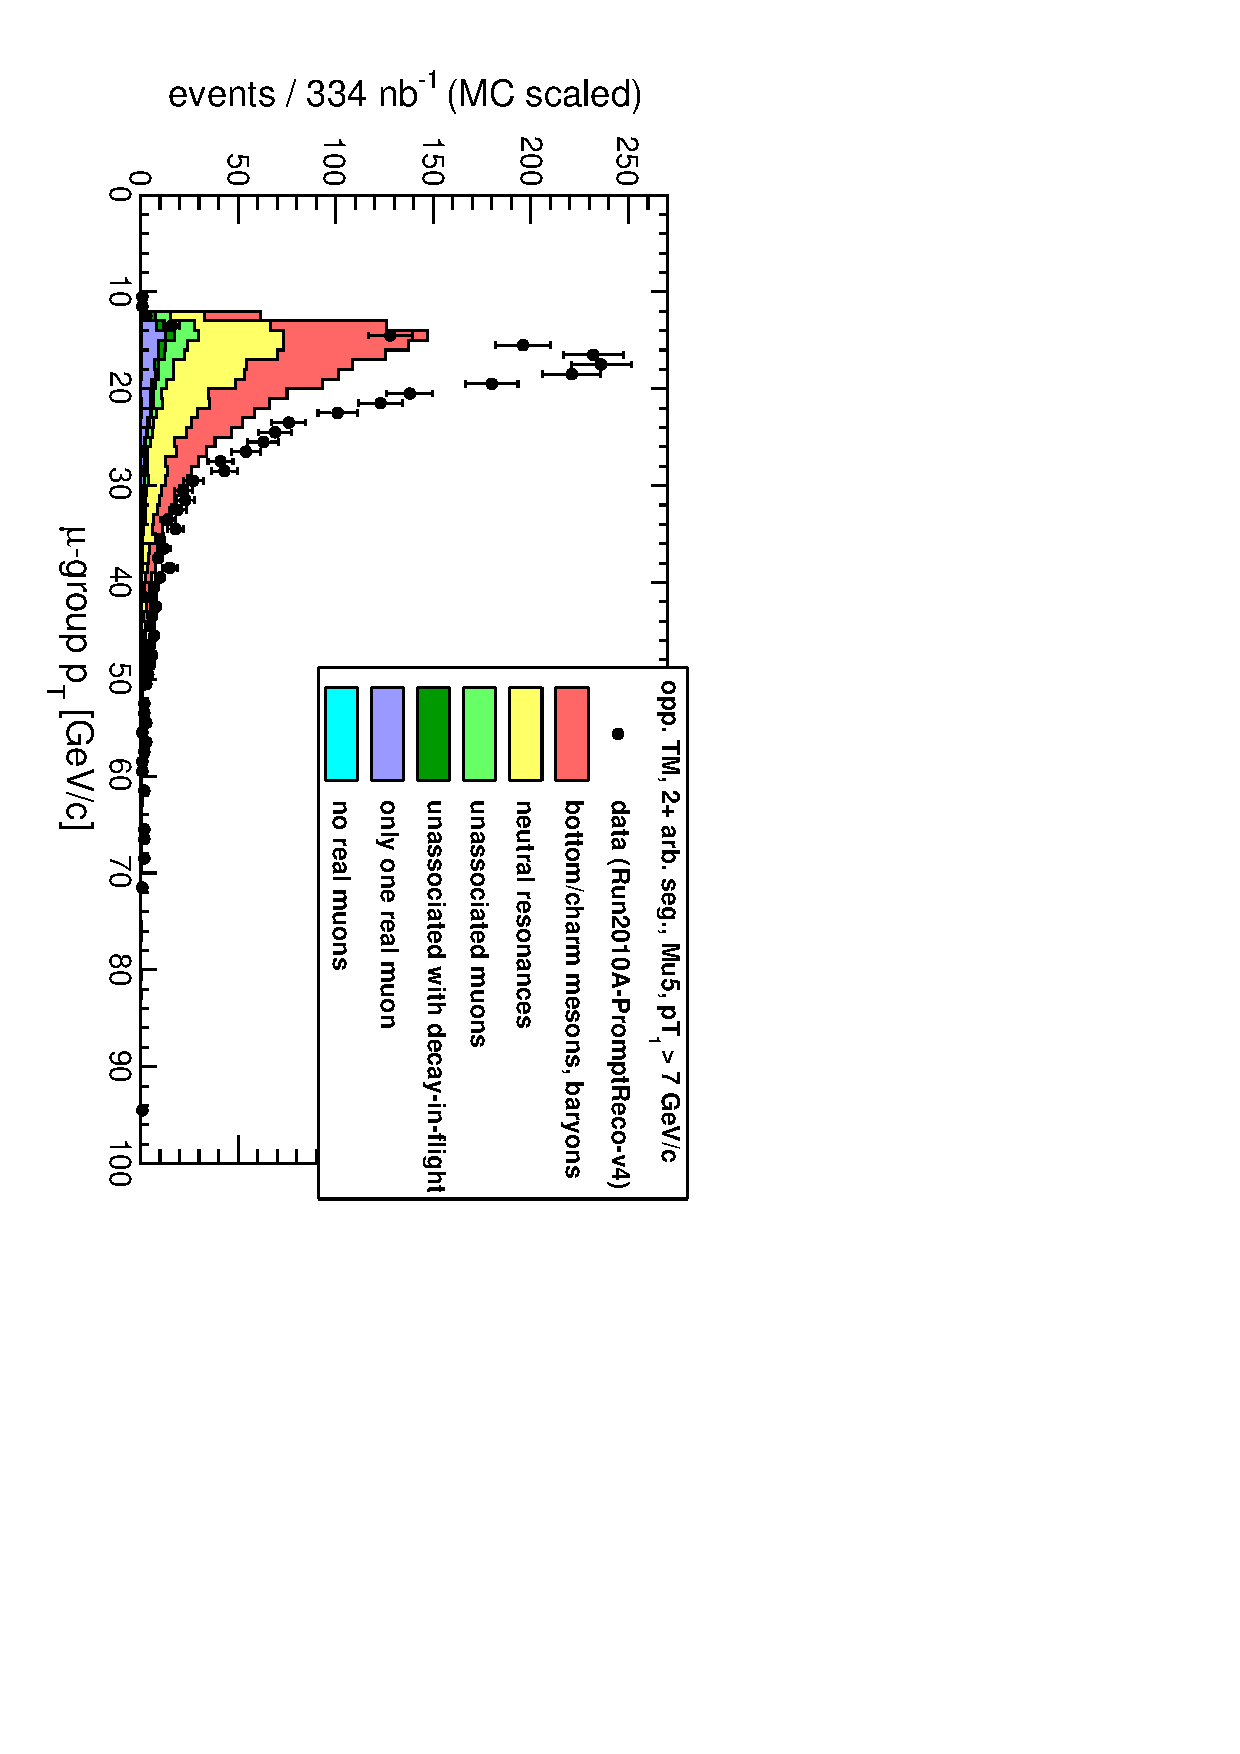
\includegraphics[height=\linewidth, angle=90]{Mu5_pt_scaled.pdf}}
\end{frame}

\begin{frame}
\frametitle{$p_T$ spectrum}
\begin{itemize}
\item In more detail: look at only $J/\psi$ mass region
\item Clearly, it's just because we're missing the prompt $J/\psi$
(and $\psi(2S)$) contributions {\scriptsize (if I include those MC
samples, then perhaps everything will line up without any
MC-tuning\ldots)}
\end{itemize}

\vfill
\includegraphics[height=\linewidth, angle=90]{Mu5_pt_jpsi.pdf}
\end{frame}

\begin{frame}
\frametitle{Gallery of resonances}

\begin{columns}
\column{0.4\linewidth}
\includegraphics[width=\linewidth]{Mu5_mass_eta.png}

\includegraphics[width=\linewidth]{Mu5_mass_omg.png}

\includegraphics[width=\linewidth]{Mu5_mass_phi.png}

\column{0.6\linewidth}
\includegraphics[width=\linewidth]{Mu5_mass_jpsi.png}

\includegraphics[width=\linewidth]{Mu5_mass_psi2s.png}

\end{columns}
\label{numpages}
\end{frame}


%% \begin{frame}
%% \frametitle{}
%% \begin{itemize}
%% \item 
%% \end{itemize}

%% \vfill
%% \includegraphics[height=\linewidth, angle=90]{Mu5_.pdf}
%% \end{frame}



%% \section*{First section}
%% \begin{frame}
%% \begin{center}
%% \Huge \textcolor{blue}{First section}
%% \end{center}
%% \end{frame}

%% \begin{frame}
%% \end{frame}

\end{document}
